\documentclass[twoside]{book}

% Packages required by doxygen
\usepackage{fixltx2e}
\usepackage{calc}
\usepackage{doxygen}
\usepackage[export]{adjustbox} % also loads graphicx
\usepackage{graphicx}
\usepackage[utf8]{inputenc}
\usepackage{makeidx}
\usepackage{multicol}
\usepackage{multirow}
\PassOptionsToPackage{warn}{textcomp}
\usepackage{textcomp}
\usepackage[nointegrals]{wasysym}
\usepackage[table]{xcolor}

% Font selection
\usepackage[T1]{fontenc}
\usepackage[scaled=.90]{helvet}
\usepackage{courier}
\usepackage{amssymb}
\usepackage{sectsty}
\renewcommand{\familydefault}{\sfdefault}
\allsectionsfont{%
  \fontseries{bc}\selectfont%
  \color{darkgray}%
}
\renewcommand{\DoxyLabelFont}{%
  \fontseries{bc}\selectfont%
  \color{darkgray}%
}
\newcommand{\+}{\discretionary{\mbox{\scriptsize$\hookleftarrow$}}{}{}}

% Page & text layout
\usepackage{geometry}
\geometry{%
  a4paper,%
  top=2.5cm,%
  bottom=2.5cm,%
  left=2.5cm,%
  right=2.5cm%
}
\tolerance=750
\hfuzz=15pt
\hbadness=750
\setlength{\emergencystretch}{15pt}
\setlength{\parindent}{0cm}
\setlength{\parskip}{3ex plus 2ex minus 2ex}
\makeatletter
\renewcommand{\paragraph}{%
  \@startsection{paragraph}{4}{0ex}{-1.0ex}{1.0ex}{%
    \normalfont\normalsize\bfseries\SS@parafont%
  }%
}
\renewcommand{\subparagraph}{%
  \@startsection{subparagraph}{5}{0ex}{-1.0ex}{1.0ex}{%
    \normalfont\normalsize\bfseries\SS@subparafont%
  }%
}
\makeatother

% Headers & footers
\usepackage{fancyhdr}
\pagestyle{fancyplain}
\fancyhead[LE]{\fancyplain{}{\bfseries\thepage}}
\fancyhead[CE]{\fancyplain{}{}}
\fancyhead[RE]{\fancyplain{}{\bfseries\leftmark}}
\fancyhead[LO]{\fancyplain{}{\bfseries\rightmark}}
\fancyhead[CO]{\fancyplain{}{}}
\fancyhead[RO]{\fancyplain{}{\bfseries\thepage}}
\fancyfoot[LE]{\fancyplain{}{}}
\fancyfoot[CE]{\fancyplain{}{}}
\fancyfoot[RE]{\fancyplain{}{\bfseries\scriptsize Generated by Doxygen }}
\fancyfoot[LO]{\fancyplain{}{\bfseries\scriptsize Generated by Doxygen }}
\fancyfoot[CO]{\fancyplain{}{}}
\fancyfoot[RO]{\fancyplain{}{}}
\renewcommand{\footrulewidth}{0.4pt}
\renewcommand{\chaptermark}[1]{%
  \markboth{#1}{}%
}
\renewcommand{\sectionmark}[1]{%
  \markright{\thesection\ #1}%
}

% Indices & bibliography
\usepackage{natbib}
\usepackage[titles]{tocloft}
\setcounter{tocdepth}{3}
\setcounter{secnumdepth}{5}
\makeindex

% Hyperlinks (required, but should be loaded last)
\usepackage{ifpdf}
\ifpdf
  \usepackage[pdftex,pagebackref=true]{hyperref}
\else
  \usepackage[ps2pdf,pagebackref=true]{hyperref}
\fi
\hypersetup{%
  colorlinks=true,%
  linkcolor=blue,%
  citecolor=blue,%
  unicode%
}

% Custom commands
\newcommand{\clearemptydoublepage}{%
  \newpage{\pagestyle{empty}\cleardoublepage}%
}

\usepackage{caption}
\captionsetup{labelsep=space,justification=centering,font={bf},singlelinecheck=off,skip=4pt,position=top}

%===== C O N T E N T S =====

\begin{document}

% Titlepage & ToC
\hypersetup{pageanchor=false,
             bookmarksnumbered=true,
             pdfencoding=unicode
            }
\pagenumbering{alph}
\begin{titlepage}
\vspace*{7cm}
\begin{center}%
{\Large Reference Manual}\\
\vspace*{1cm}
{\large Generated by Doxygen 1.8.12}\\
\end{center}
\end{titlepage}
\clearemptydoublepage
\pagenumbering{roman}
\tableofcontents
\clearemptydoublepage
\pagenumbering{arabic}
\hypersetup{pageanchor=true}

%--- Begin generated contents ---
\chapter{Hierarchical Index}
\section{Class Hierarchy}
This inheritance list is sorted roughly, but not completely, alphabetically\+:\begin{DoxyCompactList}
\item \contentsline{section}{Counter}{\pageref{class_counter}}{}
\item \contentsline{section}{External\+Merge\+Sort}{\pageref{class_external_merge_sort}}{}
\begin{DoxyCompactList}
\item \contentsline{section}{Bubble\+External\+Sort}{\pageref{class_bubble_external_sort}}{}
\item \contentsline{section}{Heap\+External\+Sort}{\pageref{class_heap_external_sort}}{}
\item \contentsline{section}{Quick\+External\+Sort}{\pageref{class_quick_external_sort}}{}
\end{DoxyCompactList}
\item \contentsline{section}{File\+Manager}{\pageref{class_file_manager}}{}
\item \contentsline{section}{User\+Interface}{\pageref{class_user_interface}}{}
\end{DoxyCompactList}

\chapter{Class Index}
\section{Классы}
Классы с их кратким описанием.\begin{DoxyCompactList}
\item\contentsline{section}{\hyperlink{class_bubble_external_sort}{Bubble\+External\+Sort} \\*Класс внешней многофазной сортировки слиянием, использующий внутреннюю пузырьковую сортировку }{\pageref{class_bubble_external_sort}}{}
\item\contentsline{section}{\hyperlink{class_counter}{Counter} \\*Класс Счетчик }{\pageref{class_counter}}{}
\item\contentsline{section}{\hyperlink{class_external_merge_sort}{External\+Merge\+Sort} \\*Класс внешней многофазной сортировки слиянием }{\pageref{class_external_merge_sort}}{}
\item\contentsline{section}{\hyperlink{class_file_manager}{File\+Manager} \\*Класс файлового менеджера }{\pageref{class_file_manager}}{}
\item\contentsline{section}{\hyperlink{class_heap_external_sort}{Heap\+External\+Sort} \\*Класс внешней многофазной сортировки слиянием, использующий внутреннюю пирамидальную сортировку }{\pageref{class_heap_external_sort}}{}
\item\contentsline{section}{\hyperlink{class_quick_external_sort}{Quick\+External\+Sort} \\*Класс внешней многофазной сортировки слиянием, использующий внутреннюю быструю сортировку }{\pageref{class_quick_external_sort}}{}
\item\contentsline{section}{\hyperlink{class_user_interface}{User\+Interface} \\*Класс пользовательского интерфейса }{\pageref{class_user_interface}}{}
\end{DoxyCompactList}

\chapter{File Index}
\section{Файлы}
Полный список файлов.\begin{DoxyCompactList}
\item\contentsline{section}{C\+:/\+Users/админ/\+Documents/\+Projects\+C++/\+External\+Merge\+Sort\+Production/\+External\+Merge\+Sort\+Production/\hyperlink{_bubble_external_sort_8cpp}{Bubble\+External\+Sort.\+cpp} }{\pageref{_bubble_external_sort_8cpp}}{}
\item\contentsline{section}{C\+:/\+Users/админ/\+Documents/\+Projects\+C++/\+External\+Merge\+Sort\+Production/\+External\+Merge\+Sort\+Production/\hyperlink{_bubble_external_sort_8h}{Bubble\+External\+Sort.\+h} }{\pageref{_bubble_external_sort_8h}}{}
\item\contentsline{section}{C\+:/\+Users/админ/\+Documents/\+Projects\+C++/\+External\+Merge\+Sort\+Production/\+External\+Merge\+Sort\+Production/\hyperlink{_counter_8cpp}{Counter.\+cpp} }{\pageref{_counter_8cpp}}{}
\item\contentsline{section}{C\+:/\+Users/админ/\+Documents/\+Projects\+C++/\+External\+Merge\+Sort\+Production/\+External\+Merge\+Sort\+Production/\hyperlink{_counter_8h}{Counter.\+h} }{\pageref{_counter_8h}}{}
\item\contentsline{section}{C\+:/\+Users/админ/\+Documents/\+Projects\+C++/\+External\+Merge\+Sort\+Production/\+External\+Merge\+Sort\+Production/\hyperlink{_external_merge_sort_8cpp}{External\+Merge\+Sort.\+cpp} }{\pageref{_external_merge_sort_8cpp}}{}
\item\contentsline{section}{C\+:/\+Users/админ/\+Documents/\+Projects\+C++/\+External\+Merge\+Sort\+Production/\+External\+Merge\+Sort\+Production/\hyperlink{_external_merge_sort_8h}{External\+Merge\+Sort.\+h} }{\pageref{_external_merge_sort_8h}}{}
\item\contentsline{section}{C\+:/\+Users/админ/\+Documents/\+Projects\+C++/\+External\+Merge\+Sort\+Production/\+External\+Merge\+Sort\+Production/\hyperlink{_external_merge_sort_production_8cpp}{External\+Merge\+Sort\+Production.\+cpp} }{\pageref{_external_merge_sort_production_8cpp}}{}
\item\contentsline{section}{C\+:/\+Users/админ/\+Documents/\+Projects\+C++/\+External\+Merge\+Sort\+Production/\+External\+Merge\+Sort\+Production/\hyperlink{_file_manager_8cpp}{File\+Manager.\+cpp} }{\pageref{_file_manager_8cpp}}{}
\item\contentsline{section}{C\+:/\+Users/админ/\+Documents/\+Projects\+C++/\+External\+Merge\+Sort\+Production/\+External\+Merge\+Sort\+Production/\hyperlink{_file_manager_8h}{File\+Manager.\+h} }{\pageref{_file_manager_8h}}{}
\item\contentsline{section}{C\+:/\+Users/админ/\+Documents/\+Projects\+C++/\+External\+Merge\+Sort\+Production/\+External\+Merge\+Sort\+Production/\hyperlink{_heap_external_sort_8cpp}{Heap\+External\+Sort.\+cpp} }{\pageref{_heap_external_sort_8cpp}}{}
\item\contentsline{section}{C\+:/\+Users/админ/\+Documents/\+Projects\+C++/\+External\+Merge\+Sort\+Production/\+External\+Merge\+Sort\+Production/\hyperlink{_heap_external_sort_8h}{Heap\+External\+Sort.\+h} }{\pageref{_heap_external_sort_8h}}{}
\item\contentsline{section}{C\+:/\+Users/админ/\+Documents/\+Projects\+C++/\+External\+Merge\+Sort\+Production/\+External\+Merge\+Sort\+Production/\hyperlink{_quick_external_sort_8cpp}{Quick\+External\+Sort.\+cpp} }{\pageref{_quick_external_sort_8cpp}}{}
\item\contentsline{section}{C\+:/\+Users/админ/\+Documents/\+Projects\+C++/\+External\+Merge\+Sort\+Production/\+External\+Merge\+Sort\+Production/\hyperlink{_quick_external_sort_8h}{Quick\+External\+Sort.\+h} }{\pageref{_quick_external_sort_8h}}{}
\item\contentsline{section}{C\+:/\+Users/админ/\+Documents/\+Projects\+C++/\+External\+Merge\+Sort\+Production/\+External\+Merge\+Sort\+Production/\hyperlink{stdafx_8cpp}{stdafx.\+cpp} }{\pageref{stdafx_8cpp}}{}
\item\contentsline{section}{C\+:/\+Users/админ/\+Documents/\+Projects\+C++/\+External\+Merge\+Sort\+Production/\+External\+Merge\+Sort\+Production/\hyperlink{stdafx_8h}{stdafx.\+h} }{\pageref{stdafx_8h}}{}
\item\contentsline{section}{C\+:/\+Users/админ/\+Documents/\+Projects\+C++/\+External\+Merge\+Sort\+Production/\+External\+Merge\+Sort\+Production/\hyperlink{_structures_8h}{Structures.\+h} }{\pageref{_structures_8h}}{}
\item\contentsline{section}{C\+:/\+Users/админ/\+Documents/\+Projects\+C++/\+External\+Merge\+Sort\+Production/\+External\+Merge\+Sort\+Production/\hyperlink{targetver_8h}{targetver.\+h} }{\pageref{targetver_8h}}{}
\item\contentsline{section}{C\+:/\+Users/админ/\+Documents/\+Projects\+C++/\+External\+Merge\+Sort\+Production/\+External\+Merge\+Sort\+Production/\hyperlink{_user_interface_8cpp}{User\+Interface.\+cpp} }{\pageref{_user_interface_8cpp}}{}
\item\contentsline{section}{C\+:/\+Users/админ/\+Documents/\+Projects\+C++/\+External\+Merge\+Sort\+Production/\+External\+Merge\+Sort\+Production/\hyperlink{_user_interface_8h}{User\+Interface.\+h} }{\pageref{_user_interface_8h}}{}
\end{DoxyCompactList}

\chapter{Class Documentation}
\hypertarget{class_bubble_external_sort}{}\section{Bubble\+External\+Sort Class Reference}
\label{class_bubble_external_sort}\index{Bubble\+External\+Sort@{Bubble\+External\+Sort}}


{\ttfamily \#include $<$Bubble\+External\+Sort.\+h$>$}

Inheritance diagram for Bubble\+External\+Sort\+:\begin{figure}[H]
\begin{center}
\leavevmode
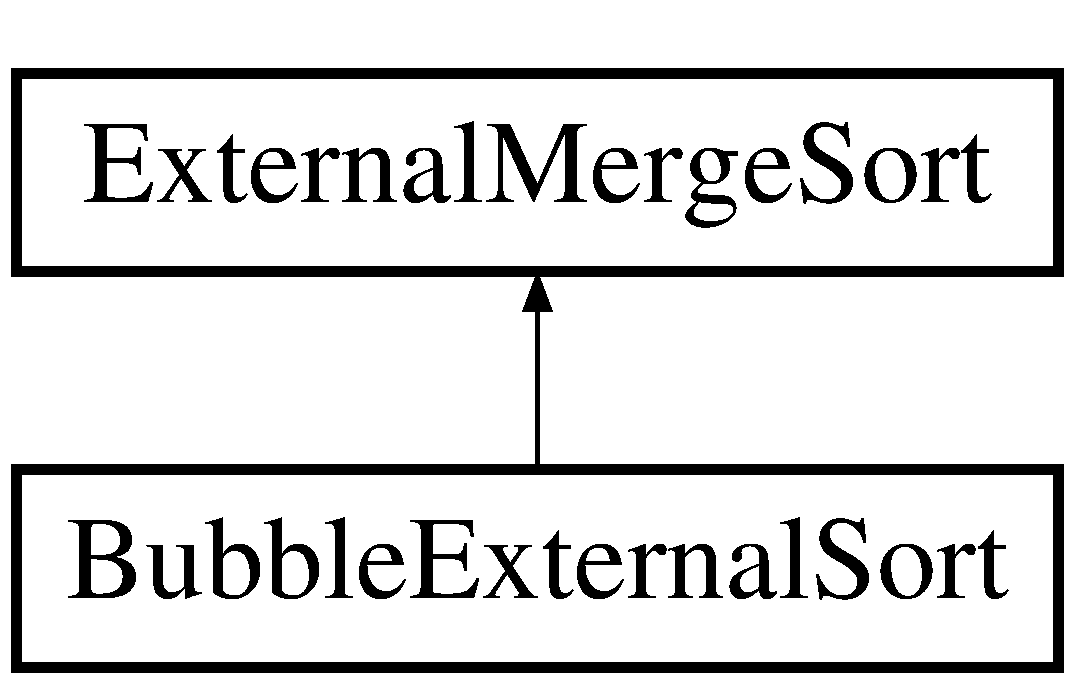
\includegraphics[height=2.000000cm]{class_bubble_external_sort}
\end{center}
\end{figure}
\subsection*{Public Member Functions}
\begin{DoxyCompactItemize}
\item 
virtual void \hyperlink{class_bubble_external_sort_ac2c8c1a8dad0f0f99a176d3641b7625c}{sort} (long long $\ast$, long long)
\item 
\hyperlink{class_bubble_external_sort_a420f93ff7677a75557f805749011f86e}{Bubble\+External\+Sort} ()
\item 
\hyperlink{class_bubble_external_sort_a2075c6e2117da937f397ceb993336e81}{$\sim$\+Bubble\+External\+Sort} ()
\end{DoxyCompactItemize}
\subsection*{Additional Inherited Members}


\subsection{Constructor \& Destructor Documentation}
\hypertarget{class_bubble_external_sort_a420f93ff7677a75557f805749011f86e}{}\label{class_bubble_external_sort_a420f93ff7677a75557f805749011f86e} 
\index{Bubble\+External\+Sort@{Bubble\+External\+Sort}!Bubble\+External\+Sort@{Bubble\+External\+Sort}}
\index{Bubble\+External\+Sort@{Bubble\+External\+Sort}!Bubble\+External\+Sort@{Bubble\+External\+Sort}}
\subsubsection{\texorpdfstring{Bubble\+External\+Sort()}{BubbleExternalSort()}}
{\footnotesize\ttfamily Bubble\+External\+Sort\+::\+Bubble\+External\+Sort (\begin{DoxyParamCaption}{ }\end{DoxyParamCaption})}

\hypertarget{class_bubble_external_sort_a2075c6e2117da937f397ceb993336e81}{}\label{class_bubble_external_sort_a2075c6e2117da937f397ceb993336e81} 
\index{Bubble\+External\+Sort@{Bubble\+External\+Sort}!````~Bubble\+External\+Sort@{$\sim$\+Bubble\+External\+Sort}}
\index{````~Bubble\+External\+Sort@{$\sim$\+Bubble\+External\+Sort}!Bubble\+External\+Sort@{Bubble\+External\+Sort}}
\subsubsection{\texorpdfstring{$\sim$\+Bubble\+External\+Sort()}{~BubbleExternalSort()}}
{\footnotesize\ttfamily Bubble\+External\+Sort\+::$\sim$\+Bubble\+External\+Sort (\begin{DoxyParamCaption}{ }\end{DoxyParamCaption})}



\subsection{Member Function Documentation}
\hypertarget{class_bubble_external_sort_ac2c8c1a8dad0f0f99a176d3641b7625c}{}\label{class_bubble_external_sort_ac2c8c1a8dad0f0f99a176d3641b7625c} 
\index{Bubble\+External\+Sort@{Bubble\+External\+Sort}!sort@{sort}}
\index{sort@{sort}!Bubble\+External\+Sort@{Bubble\+External\+Sort}}
\subsubsection{\texorpdfstring{sort()}{sort()}}
{\footnotesize\ttfamily void Bubble\+External\+Sort\+::sort (\begin{DoxyParamCaption}\item[{long long $\ast$}]{a,  }\item[{long long}]{length }\end{DoxyParamCaption})\hspace{0.3cm}{\ttfamily [virtual]}}



Implements \hyperlink{class_external_merge_sort_af6412221cc797a846243a343ccc12dba}{External\+Merge\+Sort}.



The documentation for this class was generated from the following files\+:\begin{DoxyCompactItemize}
\item 
C\+:/\+Users/админ/\+Documents/\+Projects\+C++/\+External\+Merge\+Sort\+Production/\+External\+Merge\+Sort\+Production/\hyperlink{_bubble_external_sort_8h}{Bubble\+External\+Sort.\+h}\item 
C\+:/\+Users/админ/\+Documents/\+Projects\+C++/\+External\+Merge\+Sort\+Production/\+External\+Merge\+Sort\+Production/\hyperlink{_bubble_external_sort_8cpp}{Bubble\+External\+Sort.\+cpp}\end{DoxyCompactItemize}

\hypertarget{class_counter}{}\section{Класс Counter}
\label{class_counter}\index{Counter@{Counter}}


{\ttfamily \#include $<$Counter.\+h$>$}



Граф связей класса Counter\+:\nopagebreak
\begin{figure}[H]
\begin{center}
\leavevmode
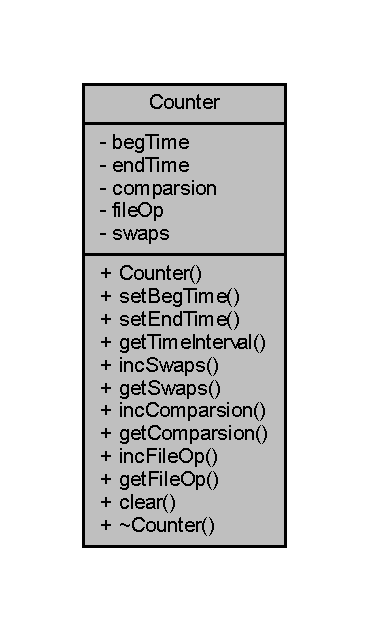
\includegraphics[width=177pt]{class_counter__coll__graph}
\end{center}
\end{figure}
\subsection*{Открытые члены}
\begin{DoxyCompactItemize}
\item 
\hyperlink{class_counter_a1e05f69b5240fbab3e7ab351672167f0}{Counter} ()
\item 
void \hyperlink{class_counter_a71dea1262b81493aa9734f62a72b2691}{set\+Beg\+Time} ()
\item 
long \hyperlink{class_counter_a338ac4f04d6f5924aa7ace3b14d9ffb9}{set\+End\+Time} ()
\item 
long \hyperlink{class_counter_a25b1a1a6cd43fb23c2d1563d5b05aec6}{get\+Time\+Interval} ()
\item 
void \hyperlink{class_counter_aa0cd30379394257e44aa7afc84ed1fce}{inc\+Swaps} ()
\item 
long \hyperlink{class_counter_af20f10e30e8bd1d078d1d66c518a814c}{get\+Swaps} ()
\item 
void \hyperlink{class_counter_a224d93150c0fe2982d3efd7aa99668e6}{inc\+Comparsion} (long long n)
\item 
long \hyperlink{class_counter_a273aaa4592ef5fae6b7a90544d0ff6e0}{get\+Comparsion} ()
\item 
void \hyperlink{class_counter_a63310182709c321ad8fe8e78b81d12aa}{inc\+File\+Op} (long long n)
\item 
long \hyperlink{class_counter_ac0a53b0296d0eacca2a2391a12ae39c5}{get\+File\+Op} ()
\item 
void \hyperlink{class_counter_af66c74ac2bc69fa4f30c34377f869596}{clear} ()
\item 
\hyperlink{class_counter_a97f4728470ae8eff37d50ef1d6bb0135}{$\sim$\+Counter} ()
\end{DoxyCompactItemize}
\subsection*{Закрытые данные}
\begin{DoxyCompactItemize}
\item 
long long \hyperlink{class_counter_ae2f8fa6947d7daa4b977d4aae2ee3c43}{beg\+Time}
\item 
long long \hyperlink{class_counter_a961ca391c9a8e3ac0efb8d6d61d734d4}{end\+Time}
\item 
long long \hyperlink{class_counter_a20f5a772c02412c338457dcc85c4a543}{comparsion}
\item 
long long \hyperlink{class_counter_abc197117fc99ab93bebc483059ae0fbc}{file\+Op}
\item 
long long \hyperlink{class_counter_a2a5ee961a25c6eb87d1ad02bcef4ade1}{swaps}
\end{DoxyCompactItemize}


\subsection{Конструктор(ы)}
\hypertarget{class_counter_a1e05f69b5240fbab3e7ab351672167f0}{}\label{class_counter_a1e05f69b5240fbab3e7ab351672167f0} 
\index{Counter@{Counter}!Counter@{Counter}}
\index{Counter@{Counter}!Counter@{Counter}}
\subsubsection{\texorpdfstring{Counter()}{Counter()}}
{\footnotesize\ttfamily Counter\+::\+Counter (\begin{DoxyParamCaption}{ }\end{DoxyParamCaption})}

Граф вызовов\+:\nopagebreak
\begin{figure}[H]
\begin{center}
\leavevmode
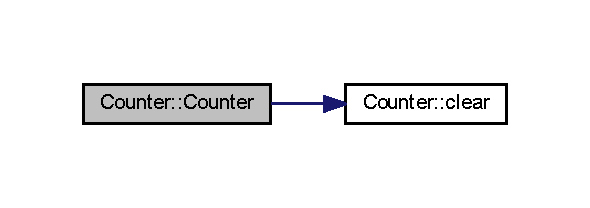
\includegraphics[width=283pt]{class_counter_a1e05f69b5240fbab3e7ab351672167f0_cgraph}
\end{center}
\end{figure}
\hypertarget{class_counter_a97f4728470ae8eff37d50ef1d6bb0135}{}\label{class_counter_a97f4728470ae8eff37d50ef1d6bb0135} 
\index{Counter@{Counter}!````~Counter@{$\sim$\+Counter}}
\index{````~Counter@{$\sim$\+Counter}!Counter@{Counter}}
\subsubsection{\texorpdfstring{$\sim$\+Counter()}{~Counter()}}
{\footnotesize\ttfamily Counter\+::$\sim$\+Counter (\begin{DoxyParamCaption}{ }\end{DoxyParamCaption})}



\subsection{Методы}
\hypertarget{class_counter_af66c74ac2bc69fa4f30c34377f869596}{}\label{class_counter_af66c74ac2bc69fa4f30c34377f869596} 
\index{Counter@{Counter}!clear@{clear}}
\index{clear@{clear}!Counter@{Counter}}
\subsubsection{\texorpdfstring{clear()}{clear()}}
{\footnotesize\ttfamily void Counter\+::clear (\begin{DoxyParamCaption}{ }\end{DoxyParamCaption})}

Граф вызова функции\+:\nopagebreak
\begin{figure}[H]
\begin{center}
\leavevmode
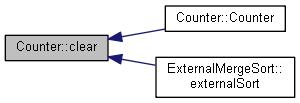
\includegraphics[width=297pt]{class_counter_af66c74ac2bc69fa4f30c34377f869596_icgraph}
\end{center}
\end{figure}
\hypertarget{class_counter_a273aaa4592ef5fae6b7a90544d0ff6e0}{}\label{class_counter_a273aaa4592ef5fae6b7a90544d0ff6e0} 
\index{Counter@{Counter}!get\+Comparsion@{get\+Comparsion}}
\index{get\+Comparsion@{get\+Comparsion}!Counter@{Counter}}
\subsubsection{\texorpdfstring{get\+Comparsion()}{getComparsion()}}
{\footnotesize\ttfamily long Counter\+::get\+Comparsion (\begin{DoxyParamCaption}{ }\end{DoxyParamCaption})}

\hypertarget{class_counter_ac0a53b0296d0eacca2a2391a12ae39c5}{}\label{class_counter_ac0a53b0296d0eacca2a2391a12ae39c5} 
\index{Counter@{Counter}!get\+File\+Op@{get\+File\+Op}}
\index{get\+File\+Op@{get\+File\+Op}!Counter@{Counter}}
\subsubsection{\texorpdfstring{get\+File\+Op()}{getFileOp()}}
{\footnotesize\ttfamily long Counter\+::get\+File\+Op (\begin{DoxyParamCaption}{ }\end{DoxyParamCaption})}

\hypertarget{class_counter_af20f10e30e8bd1d078d1d66c518a814c}{}\label{class_counter_af20f10e30e8bd1d078d1d66c518a814c} 
\index{Counter@{Counter}!get\+Swaps@{get\+Swaps}}
\index{get\+Swaps@{get\+Swaps}!Counter@{Counter}}
\subsubsection{\texorpdfstring{get\+Swaps()}{getSwaps()}}
{\footnotesize\ttfamily long Counter\+::get\+Swaps (\begin{DoxyParamCaption}{ }\end{DoxyParamCaption})}

\hypertarget{class_counter_a25b1a1a6cd43fb23c2d1563d5b05aec6}{}\label{class_counter_a25b1a1a6cd43fb23c2d1563d5b05aec6} 
\index{Counter@{Counter}!get\+Time\+Interval@{get\+Time\+Interval}}
\index{get\+Time\+Interval@{get\+Time\+Interval}!Counter@{Counter}}
\subsubsection{\texorpdfstring{get\+Time\+Interval()}{getTimeInterval()}}
{\footnotesize\ttfamily long Counter\+::get\+Time\+Interval (\begin{DoxyParamCaption}{ }\end{DoxyParamCaption})}

Граф вызова функции\+:\nopagebreak
\begin{figure}[H]
\begin{center}
\leavevmode
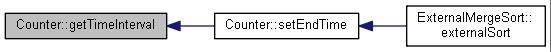
\includegraphics[width=350pt]{class_counter_a25b1a1a6cd43fb23c2d1563d5b05aec6_icgraph}
\end{center}
\end{figure}
\hypertarget{class_counter_a224d93150c0fe2982d3efd7aa99668e6}{}\label{class_counter_a224d93150c0fe2982d3efd7aa99668e6} 
\index{Counter@{Counter}!inc\+Comparsion@{inc\+Comparsion}}
\index{inc\+Comparsion@{inc\+Comparsion}!Counter@{Counter}}
\subsubsection{\texorpdfstring{inc\+Comparsion()}{incComparsion()}}
{\footnotesize\ttfamily void Counter\+::inc\+Comparsion (\begin{DoxyParamCaption}\item[{long long}]{n }\end{DoxyParamCaption})}

Граф вызова функции\+:\nopagebreak
\begin{figure}[H]
\begin{center}
\leavevmode
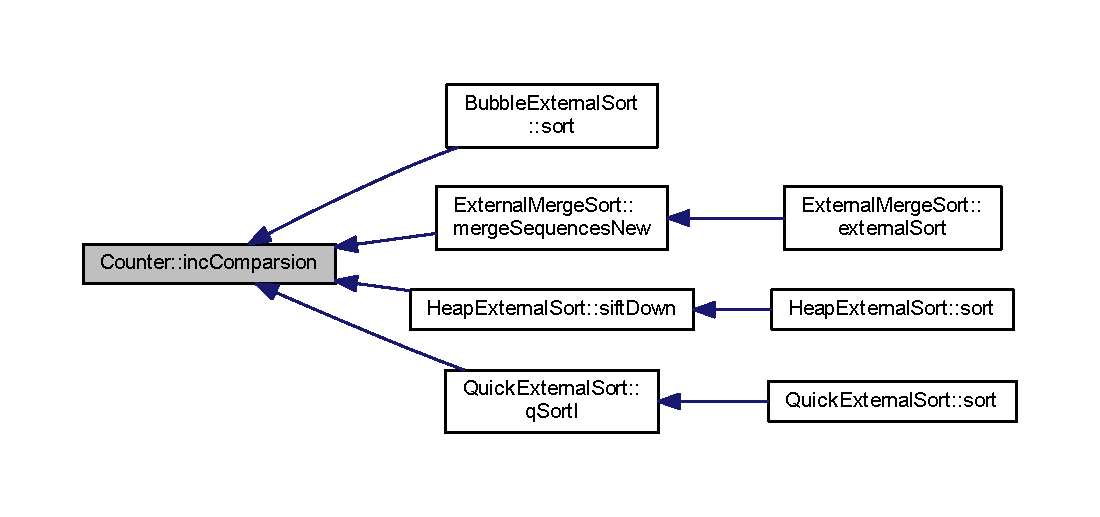
\includegraphics[width=350pt]{class_counter_a224d93150c0fe2982d3efd7aa99668e6_icgraph}
\end{center}
\end{figure}
\hypertarget{class_counter_a63310182709c321ad8fe8e78b81d12aa}{}\label{class_counter_a63310182709c321ad8fe8e78b81d12aa} 
\index{Counter@{Counter}!inc\+File\+Op@{inc\+File\+Op}}
\index{inc\+File\+Op@{inc\+File\+Op}!Counter@{Counter}}
\subsubsection{\texorpdfstring{inc\+File\+Op()}{incFileOp()}}
{\footnotesize\ttfamily void Counter\+::inc\+File\+Op (\begin{DoxyParamCaption}\item[{long long}]{n }\end{DoxyParamCaption})}

Граф вызова функции\+:\nopagebreak
\begin{figure}[H]
\begin{center}
\leavevmode
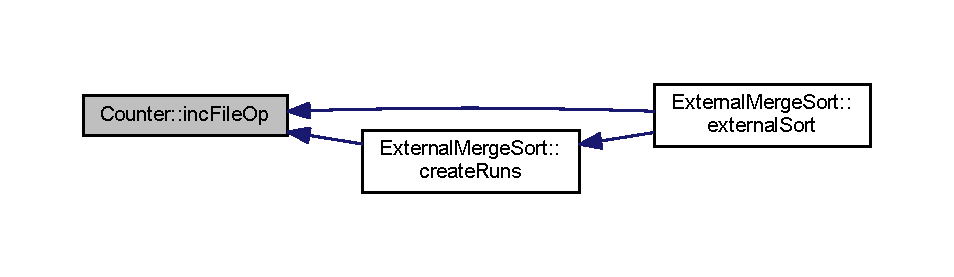
\includegraphics[width=350pt]{class_counter_a63310182709c321ad8fe8e78b81d12aa_icgraph}
\end{center}
\end{figure}
\hypertarget{class_counter_aa0cd30379394257e44aa7afc84ed1fce}{}\label{class_counter_aa0cd30379394257e44aa7afc84ed1fce} 
\index{Counter@{Counter}!inc\+Swaps@{inc\+Swaps}}
\index{inc\+Swaps@{inc\+Swaps}!Counter@{Counter}}
\subsubsection{\texorpdfstring{inc\+Swaps()}{incSwaps()}}
{\footnotesize\ttfamily void Counter\+::inc\+Swaps (\begin{DoxyParamCaption}{ }\end{DoxyParamCaption})}

Граф вызова функции\+:\nopagebreak
\begin{figure}[H]
\begin{center}
\leavevmode
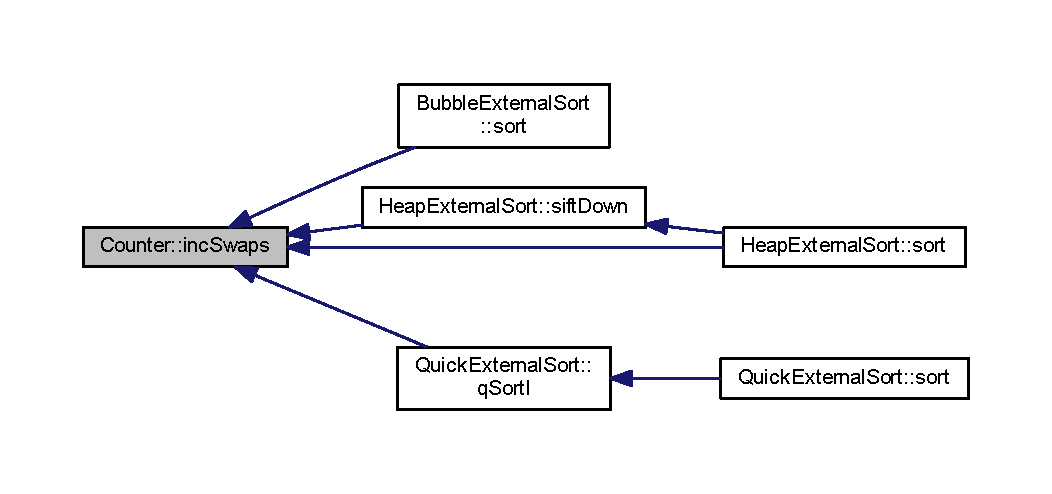
\includegraphics[width=350pt]{class_counter_aa0cd30379394257e44aa7afc84ed1fce_icgraph}
\end{center}
\end{figure}
\hypertarget{class_counter_a71dea1262b81493aa9734f62a72b2691}{}\label{class_counter_a71dea1262b81493aa9734f62a72b2691} 
\index{Counter@{Counter}!set\+Beg\+Time@{set\+Beg\+Time}}
\index{set\+Beg\+Time@{set\+Beg\+Time}!Counter@{Counter}}
\subsubsection{\texorpdfstring{set\+Beg\+Time()}{setBegTime()}}
{\footnotesize\ttfamily void Counter\+::set\+Beg\+Time (\begin{DoxyParamCaption}{ }\end{DoxyParamCaption})}

Граф вызова функции\+:\nopagebreak
\begin{figure}[H]
\begin{center}
\leavevmode
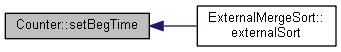
\includegraphics[width=328pt]{class_counter_a71dea1262b81493aa9734f62a72b2691_icgraph}
\end{center}
\end{figure}
\hypertarget{class_counter_a338ac4f04d6f5924aa7ace3b14d9ffb9}{}\label{class_counter_a338ac4f04d6f5924aa7ace3b14d9ffb9} 
\index{Counter@{Counter}!set\+End\+Time@{set\+End\+Time}}
\index{set\+End\+Time@{set\+End\+Time}!Counter@{Counter}}
\subsubsection{\texorpdfstring{set\+End\+Time()}{setEndTime()}}
{\footnotesize\ttfamily long Counter\+::set\+End\+Time (\begin{DoxyParamCaption}{ }\end{DoxyParamCaption})}

Граф вызовов\+:\nopagebreak
\begin{figure}[H]
\begin{center}
\leavevmode
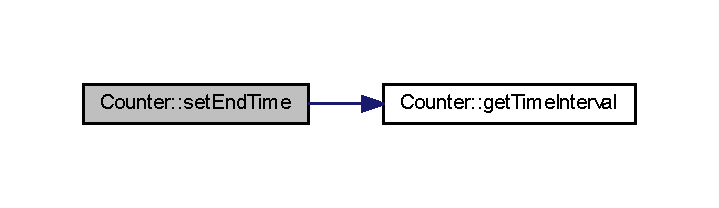
\includegraphics[width=345pt]{class_counter_a338ac4f04d6f5924aa7ace3b14d9ffb9_cgraph}
\end{center}
\end{figure}
Граф вызова функции\+:\nopagebreak
\begin{figure}[H]
\begin{center}
\leavevmode
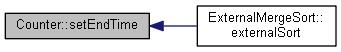
\includegraphics[width=328pt]{class_counter_a338ac4f04d6f5924aa7ace3b14d9ffb9_icgraph}
\end{center}
\end{figure}


\subsection{Данные класса}
\hypertarget{class_counter_ae2f8fa6947d7daa4b977d4aae2ee3c43}{}\label{class_counter_ae2f8fa6947d7daa4b977d4aae2ee3c43} 
\index{Counter@{Counter}!beg\+Time@{beg\+Time}}
\index{beg\+Time@{beg\+Time}!Counter@{Counter}}
\subsubsection{\texorpdfstring{beg\+Time}{begTime}}
{\footnotesize\ttfamily long long Counter\+::beg\+Time\hspace{0.3cm}{\ttfamily [private]}}

\hypertarget{class_counter_a20f5a772c02412c338457dcc85c4a543}{}\label{class_counter_a20f5a772c02412c338457dcc85c4a543} 
\index{Counter@{Counter}!comparsion@{comparsion}}
\index{comparsion@{comparsion}!Counter@{Counter}}
\subsubsection{\texorpdfstring{comparsion}{comparsion}}
{\footnotesize\ttfamily long long Counter\+::comparsion\hspace{0.3cm}{\ttfamily [private]}}

\hypertarget{class_counter_a961ca391c9a8e3ac0efb8d6d61d734d4}{}\label{class_counter_a961ca391c9a8e3ac0efb8d6d61d734d4} 
\index{Counter@{Counter}!end\+Time@{end\+Time}}
\index{end\+Time@{end\+Time}!Counter@{Counter}}
\subsubsection{\texorpdfstring{end\+Time}{endTime}}
{\footnotesize\ttfamily long long Counter\+::end\+Time\hspace{0.3cm}{\ttfamily [private]}}

\hypertarget{class_counter_abc197117fc99ab93bebc483059ae0fbc}{}\label{class_counter_abc197117fc99ab93bebc483059ae0fbc} 
\index{Counter@{Counter}!file\+Op@{file\+Op}}
\index{file\+Op@{file\+Op}!Counter@{Counter}}
\subsubsection{\texorpdfstring{file\+Op}{fileOp}}
{\footnotesize\ttfamily long long Counter\+::file\+Op\hspace{0.3cm}{\ttfamily [private]}}

\hypertarget{class_counter_a2a5ee961a25c6eb87d1ad02bcef4ade1}{}\label{class_counter_a2a5ee961a25c6eb87d1ad02bcef4ade1} 
\index{Counter@{Counter}!swaps@{swaps}}
\index{swaps@{swaps}!Counter@{Counter}}
\subsubsection{\texorpdfstring{swaps}{swaps}}
{\footnotesize\ttfamily long long Counter\+::swaps\hspace{0.3cm}{\ttfamily [private]}}



Объявления и описания членов классов находятся в файлах\+:\begin{DoxyCompactItemize}
\item 
C\+:/\+Users/админ/\+Documents/\+Projects\+C++/\+External\+Merge\+Sort\+Production/\+External\+Merge\+Sort\+Production/\hyperlink{_counter_8h}{Counter.\+h}\item 
C\+:/\+Users/админ/\+Documents/\+Projects\+C++/\+External\+Merge\+Sort\+Production/\+External\+Merge\+Sort\+Production/\hyperlink{_counter_8cpp}{Counter.\+cpp}\end{DoxyCompactItemize}

\hypertarget{class_external_merge_sort}{}\section{Класс External\+Merge\+Sort}
\label{class_external_merge_sort}\index{External\+Merge\+Sort@{External\+Merge\+Sort}}


\subsection{Подробное описание}
Класс внешней многофазной сортировки слиянием. 

\begin{DoxyAuthor}{Автор}
Alexander Filippov 
\end{DoxyAuthor}
\begin{DoxyDate}{Дата}
Ноябрь 2016 года
\end{DoxyDate}
Класс, осуществляющий внешнюю многофазную сортировку слиянием. Содержит в себе основные методы внешней сортировки слиянием. Виртуальная функция sort(...) переопределена в производных классах. 

{\ttfamily \#include $<$External\+Merge\+Sort.\+h$>$}



Граф наследования\+:External\+Merge\+Sort\+:\nopagebreak
\begin{figure}[H]
\begin{center}
\leavevmode
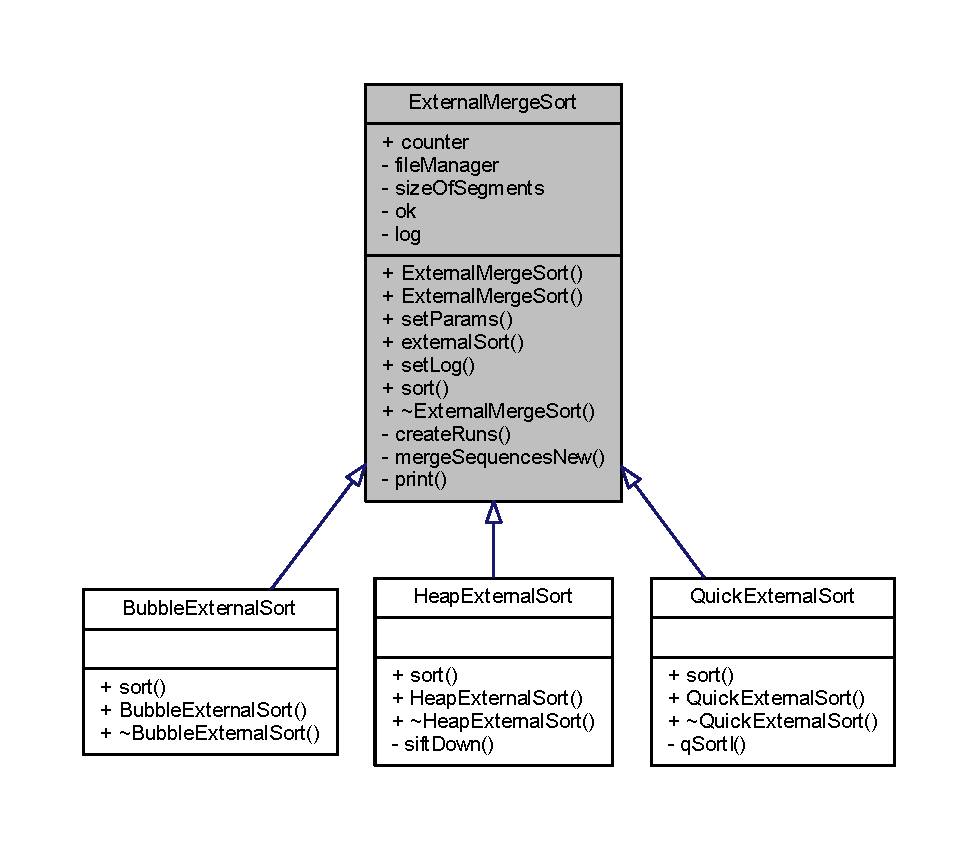
\includegraphics[width=350pt]{class_external_merge_sort__inherit__graph}
\end{center}
\end{figure}


Граф связей класса External\+Merge\+Sort\+:\nopagebreak
\begin{figure}[H]
\begin{center}
\leavevmode
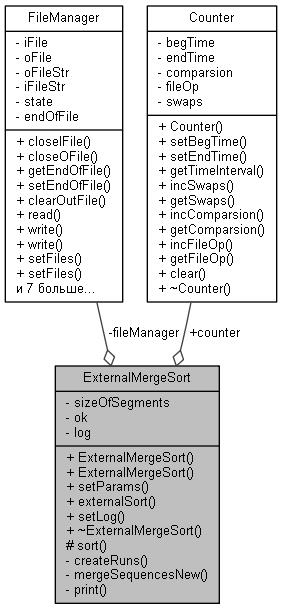
\includegraphics[width=284pt]{class_external_merge_sort__coll__graph}
\end{center}
\end{figure}
\subsection*{Открытые члены}
\begin{DoxyCompactItemize}
\item 
\hyperlink{class_external_merge_sort_a7b6efcd2abbf59a8983f972c52d04650}{External\+Merge\+Sort} ()
\begin{DoxyCompactList}\small\item\em Пустой конструктор класса. \end{DoxyCompactList}\item 
\hyperlink{class_external_merge_sort_a37df182916b341d5466f2fff0d50dfed}{External\+Merge\+Sort} (\hyperlink{class_file_manager}{File\+Manager} $\ast$file, long long \hyperlink{class_external_merge_sort_a1d68bb5e0373cf16807a41272dff1a99}{size\+Of\+Segments})
\begin{DoxyCompactList}\small\item\em Конструктор класса. \end{DoxyCompactList}\item 
\hyperlink{_structures_8h_a9864d6ef28dd6e38416afac4426b3491}{Responce} \hyperlink{class_external_merge_sort_a2a27571acdf4f42e34798663e37f5e0b}{set\+Params} (\hyperlink{class_file_manager}{File\+Manager} $\ast$file, long long \hyperlink{class_external_merge_sort_a1d68bb5e0373cf16807a41272dff1a99}{size\+Of\+Segments})
\begin{DoxyCompactList}\small\item\em Определение параметров сортировки. \end{DoxyCompactList}\item 
\hyperlink{_structures_8h_a9864d6ef28dd6e38416afac4426b3491}{Responce} \hyperlink{class_external_merge_sort_aa0d80e41effe3a13c0d63b33e208918f}{external\+Sort} ()
\begin{DoxyCompactList}\small\item\em Вызывает метод внешней многофазной сортировки. \end{DoxyCompactList}\item 
void \hyperlink{class_external_merge_sort_ac0eeaba67ee0703acf73a8a5bf78ebe1}{set\+Log} (\hyperlink{_structures_8h_af67907baa897e9fb84df0cb89795b87c}{Log\+Type} \hyperlink{class_external_merge_sort_a41f61c3beb7dc529d7f2a8b2b4ee380b}{log})
\begin{DoxyCompactList}\small\item\em Устанавливает тип логгирования. \end{DoxyCompactList}\item 
virtual \hyperlink{class_external_merge_sort_adfee7073120e0ae832c96977440b2fb4}{$\sim$\+External\+Merge\+Sort} ()
\begin{DoxyCompactList}\small\item\em Пустой виртуальный деструктор класса. \end{DoxyCompactList}\end{DoxyCompactItemize}
\subsection*{Открытые атрибуты}
\begin{DoxyCompactItemize}
\item 
\hyperlink{class_counter}{Counter} \hyperlink{class_external_merge_sort_ac9cb039a5cda56e66aecbc17465dd237}{counter}
\begin{DoxyCompactList}\small\item\em Счетчик. \end{DoxyCompactList}\end{DoxyCompactItemize}
\subsection*{Защищенные члены}
\begin{DoxyCompactItemize}
\item 
virtual void \hyperlink{class_external_merge_sort_a7b777f22151fdd869624d8aa5a39a7bb}{sort} (long long $\ast$arr, long long size)=0
\begin{DoxyCompactList}\small\item\em Сортирует последовательность длиной size одним из методов, перегруженных в производных классах. \end{DoxyCompactList}\end{DoxyCompactItemize}
\subsection*{Закрытые члены}
\begin{DoxyCompactItemize}
\item 
\hyperlink{_structures_8h_a9864d6ef28dd6e38416afac4426b3491}{Responce} \hyperlink{class_external_merge_sort_aa3ec5ccebe04f02538ee42d0ffe7b75c}{create\+Runs} (long long $\ast$size)
\begin{DoxyCompactList}\small\item\em Чтение входной последовательности из файла. \end{DoxyCompactList}\item 
\hyperlink{_structures_8h_a9864d6ef28dd6e38416afac4426b3491}{Responce} \hyperlink{class_external_merge_sort_a8b4f951d9ee53818b8d3d4e84e2a1aa4}{merge\+Sequences\+New} (\hyperlink{class_file_manager}{File\+Manager} $\ast$input1, \hyperlink{class_file_manager}{File\+Manager} $\ast$input2, \hyperlink{class_file_manager}{File\+Manager} $\ast$out, long long size)
\begin{DoxyCompactList}\small\item\em Слияние последовательностей. \end{DoxyCompactList}\item 
void \hyperlink{class_external_merge_sort_a7a6b94fff35130ed6a498f9a31d0f863}{print} (const char $\ast$msg)
\begin{DoxyCompactList}\small\item\em Логгирование. \end{DoxyCompactList}\end{DoxyCompactItemize}
\subsection*{Закрытые данные}
\begin{DoxyCompactItemize}
\item 
\hyperlink{class_file_manager}{File\+Manager} $\ast$ \hyperlink{class_external_merge_sort_ab82d3b62a57be6c80dbd12b90de278e2}{file\+Manager}
\begin{DoxyCompactList}\small\item\em Указатель на класс файл-\/менеджера. \end{DoxyCompactList}\item 
long long \hyperlink{class_external_merge_sort_a1d68bb5e0373cf16807a41272dff1a99}{size\+Of\+Segments}
\begin{DoxyCompactList}\small\item\em Размер сегментов. \end{DoxyCompactList}\item 
bool \hyperlink{class_external_merge_sort_a4b050cd230e144a11f65e57523e15ce6}{ok}
\begin{DoxyCompactList}\small\item\em Флаг готовности сортировки. \end{DoxyCompactList}\item 
\hyperlink{_structures_8h_af67907baa897e9fb84df0cb89795b87c}{Log\+Type} \hyperlink{class_external_merge_sort_a41f61c3beb7dc529d7f2a8b2b4ee380b}{log}
\begin{DoxyCompactList}\small\item\em Тип логгирования. \end{DoxyCompactList}\end{DoxyCompactItemize}


\subsection{Конструктор(ы)}
\hypertarget{class_external_merge_sort_a7b6efcd2abbf59a8983f972c52d04650}{}\label{class_external_merge_sort_a7b6efcd2abbf59a8983f972c52d04650} 
\index{External\+Merge\+Sort@{External\+Merge\+Sort}!External\+Merge\+Sort@{External\+Merge\+Sort}}
\index{External\+Merge\+Sort@{External\+Merge\+Sort}!External\+Merge\+Sort@{External\+Merge\+Sort}}
\subsubsection{\texorpdfstring{External\+Merge\+Sort()}{ExternalMergeSort()}\hspace{0.1cm}{\footnotesize\ttfamily [1/2]}}
{\footnotesize\ttfamily External\+Merge\+Sort\+::\+External\+Merge\+Sort (\begin{DoxyParamCaption}{ }\end{DoxyParamCaption})}



Пустой конструктор класса. 

Обнуляет атрибуты. \hypertarget{class_external_merge_sort_a37df182916b341d5466f2fff0d50dfed}{}\label{class_external_merge_sort_a37df182916b341d5466f2fff0d50dfed} 
\index{External\+Merge\+Sort@{External\+Merge\+Sort}!External\+Merge\+Sort@{External\+Merge\+Sort}}
\index{External\+Merge\+Sort@{External\+Merge\+Sort}!External\+Merge\+Sort@{External\+Merge\+Sort}}
\subsubsection{\texorpdfstring{External\+Merge\+Sort()}{ExternalMergeSort()}\hspace{0.1cm}{\footnotesize\ttfamily [2/2]}}
{\footnotesize\ttfamily External\+Merge\+Sort\+::\+External\+Merge\+Sort (\begin{DoxyParamCaption}\item[{\hyperlink{class_file_manager}{File\+Manager} $\ast$}]{file,  }\item[{long long}]{size\+Of\+Segments }\end{DoxyParamCaption})}



Конструктор класса. 


\begin{DoxyParams}[1]{Аргументы}
\mbox{\tt in}  & {\em file} & Файл-\/менеджер, отвечающий за взаимодействие сортировки с файловой системой. \\
\hline
\mbox{\tt in}  & {\em size\+Of\+Segments} & Размер сегментов.\\
\hline
\end{DoxyParams}
Вызывет set\+Params(...), если код возврата не Success, бросает исключение. Граф вызовов\+:\nopagebreak
\begin{figure}[H]
\begin{center}
\leavevmode
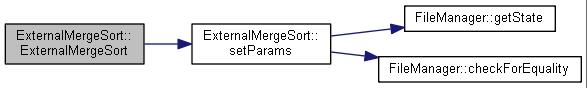
\includegraphics[width=350pt]{class_external_merge_sort_a37df182916b341d5466f2fff0d50dfed_cgraph}
\end{center}
\end{figure}
\hypertarget{class_external_merge_sort_adfee7073120e0ae832c96977440b2fb4}{}\label{class_external_merge_sort_adfee7073120e0ae832c96977440b2fb4} 
\index{External\+Merge\+Sort@{External\+Merge\+Sort}!````~External\+Merge\+Sort@{$\sim$\+External\+Merge\+Sort}}
\index{````~External\+Merge\+Sort@{$\sim$\+External\+Merge\+Sort}!External\+Merge\+Sort@{External\+Merge\+Sort}}
\subsubsection{\texorpdfstring{$\sim$\+External\+Merge\+Sort()}{~ExternalMergeSort()}}
{\footnotesize\ttfamily External\+Merge\+Sort\+::$\sim$\+External\+Merge\+Sort (\begin{DoxyParamCaption}{ }\end{DoxyParamCaption})\hspace{0.3cm}{\ttfamily [virtual]}}



Пустой виртуальный деструктор класса. 

Освобождает выделенную память. 

\subsection{Методы}
\hypertarget{class_external_merge_sort_aa3ec5ccebe04f02538ee42d0ffe7b75c}{}\label{class_external_merge_sort_aa3ec5ccebe04f02538ee42d0ffe7b75c} 
\index{External\+Merge\+Sort@{External\+Merge\+Sort}!create\+Runs@{create\+Runs}}
\index{create\+Runs@{create\+Runs}!External\+Merge\+Sort@{External\+Merge\+Sort}}
\subsubsection{\texorpdfstring{create\+Runs()}{createRuns()}}
{\footnotesize\ttfamily \hyperlink{_structures_8h_a9864d6ef28dd6e38416afac4426b3491}{Responce} External\+Merge\+Sort\+::create\+Runs (\begin{DoxyParamCaption}\item[{long long $\ast$}]{size }\end{DoxyParamCaption})\hspace{0.3cm}{\ttfamily [private]}}



Чтение входной последовательности из файла. 


\begin{DoxyParams}[1]{Аргументы}
\mbox{\tt out}  & {\em size} & Размер входной последовательности. \\
\hline
\end{DoxyParams}
\begin{DoxyReturn}{Возвращает}
Код успеха или ошибки.
\end{DoxyReturn}
Считывает последовательности длиной size, сортирует их методом перегруженным в производных классах и записывает в один из буферных файлов. Граф вызовов\+:\nopagebreak
\begin{figure}[H]
\begin{center}
\leavevmode
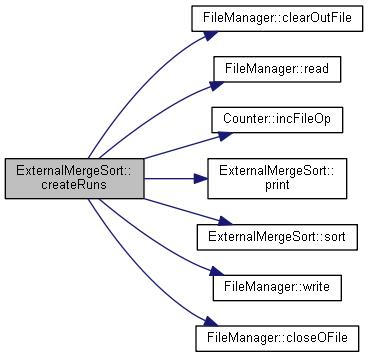
\includegraphics[width=348pt]{class_external_merge_sort_aa3ec5ccebe04f02538ee42d0ffe7b75c_cgraph}
\end{center}
\end{figure}
Граф вызова функции\+:\nopagebreak
\begin{figure}[H]
\begin{center}
\leavevmode
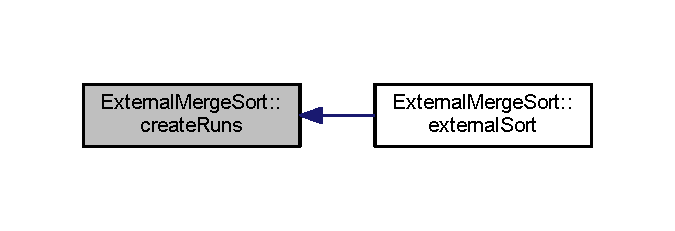
\includegraphics[width=324pt]{class_external_merge_sort_aa3ec5ccebe04f02538ee42d0ffe7b75c_icgraph}
\end{center}
\end{figure}
\hypertarget{class_external_merge_sort_aa0d80e41effe3a13c0d63b33e208918f}{}\label{class_external_merge_sort_aa0d80e41effe3a13c0d63b33e208918f} 
\index{External\+Merge\+Sort@{External\+Merge\+Sort}!external\+Sort@{external\+Sort}}
\index{external\+Sort@{external\+Sort}!External\+Merge\+Sort@{External\+Merge\+Sort}}
\subsubsection{\texorpdfstring{external\+Sort()}{externalSort()}}
{\footnotesize\ttfamily \hyperlink{_structures_8h_a9864d6ef28dd6e38416afac4426b3491}{Responce} External\+Merge\+Sort\+::external\+Sort (\begin{DoxyParamCaption}{ }\end{DoxyParamCaption})}



Вызывает метод внешней многофазной сортировки. 

\begin{DoxyReturn}{Возвращает}
Код успеха или ошибки.
\end{DoxyReturn}
Осуществляет внешнюю многофазную сортировку слиянием. Вызывает create\+Runs(...), merge\+Sequnces\+New(...). Граф вызовов\+:\nopagebreak
\begin{figure}[H]
\begin{center}
\leavevmode
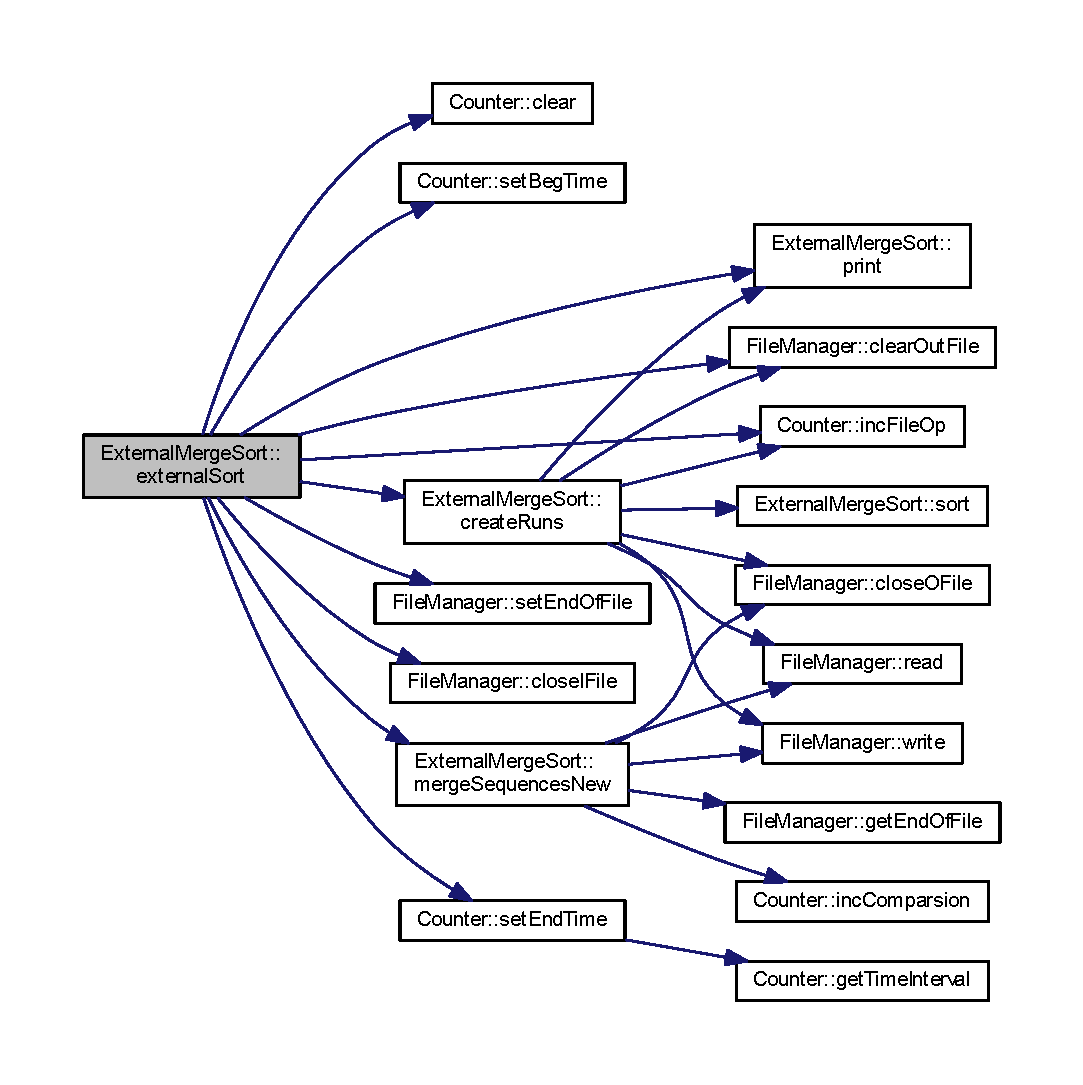
\includegraphics[width=350pt]{class_external_merge_sort_aa0d80e41effe3a13c0d63b33e208918f_cgraph}
\end{center}
\end{figure}
\hypertarget{class_external_merge_sort_a8b4f951d9ee53818b8d3d4e84e2a1aa4}{}\label{class_external_merge_sort_a8b4f951d9ee53818b8d3d4e84e2a1aa4} 
\index{External\+Merge\+Sort@{External\+Merge\+Sort}!merge\+Sequences\+New@{merge\+Sequences\+New}}
\index{merge\+Sequences\+New@{merge\+Sequences\+New}!External\+Merge\+Sort@{External\+Merge\+Sort}}
\subsubsection{\texorpdfstring{merge\+Sequences\+New()}{mergeSequencesNew()}}
{\footnotesize\ttfamily \hyperlink{_structures_8h_a9864d6ef28dd6e38416afac4426b3491}{Responce} External\+Merge\+Sort\+::merge\+Sequences\+New (\begin{DoxyParamCaption}\item[{\hyperlink{class_file_manager}{File\+Manager} $\ast$}]{input1,  }\item[{\hyperlink{class_file_manager}{File\+Manager} $\ast$}]{input2,  }\item[{\hyperlink{class_file_manager}{File\+Manager} $\ast$}]{out,  }\item[{long long}]{size }\end{DoxyParamCaption})\hspace{0.3cm}{\ttfamily [private]}}



Слияние последовательностей. 


\begin{DoxyParams}[1]{Аргументы}
\mbox{\tt in}  & {\em input1} & Первый входной файл. \\
\hline
\mbox{\tt in}  & {\em input2} & Второй входной файл. \\
\hline
\mbox{\tt in}  & {\em out} & Выходной файл. \\
\hline
\mbox{\tt in}  & {\em size} & Размер сегментов \\
\hline
\end{DoxyParams}
\begin{DoxyReturn}{Возвращает}
Код успеха или ошибки.
\end{DoxyReturn}
Сливает последовательность длиной size из input1 с последовательностью длиной sizr из input2, результат записывает в out. Граф вызовов\+:\nopagebreak
\begin{figure}[H]
\begin{center}
\leavevmode
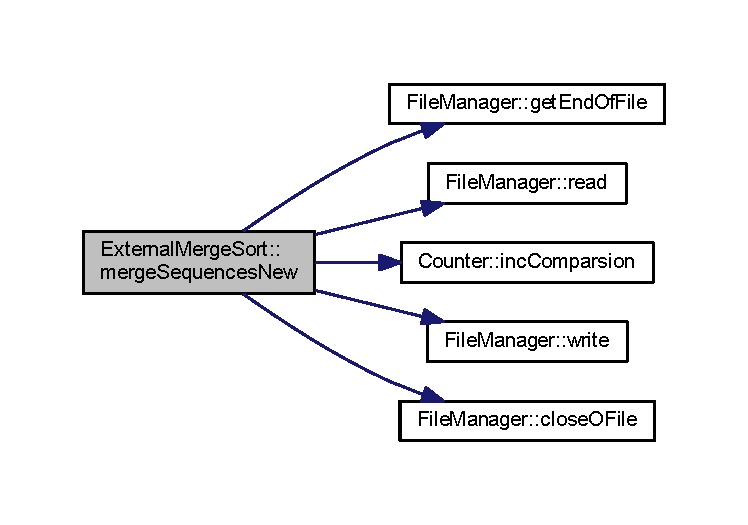
\includegraphics[width=350pt]{class_external_merge_sort_a8b4f951d9ee53818b8d3d4e84e2a1aa4_cgraph}
\end{center}
\end{figure}
Граф вызова функции\+:\nopagebreak
\begin{figure}[H]
\begin{center}
\leavevmode
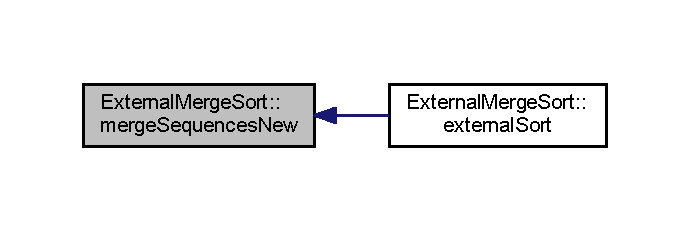
\includegraphics[width=331pt]{class_external_merge_sort_a8b4f951d9ee53818b8d3d4e84e2a1aa4_icgraph}
\end{center}
\end{figure}
\hypertarget{class_external_merge_sort_a7a6b94fff35130ed6a498f9a31d0f863}{}\label{class_external_merge_sort_a7a6b94fff35130ed6a498f9a31d0f863} 
\index{External\+Merge\+Sort@{External\+Merge\+Sort}!print@{print}}
\index{print@{print}!External\+Merge\+Sort@{External\+Merge\+Sort}}
\subsubsection{\texorpdfstring{print()}{print()}}
{\footnotesize\ttfamily void External\+Merge\+Sort\+::print (\begin{DoxyParamCaption}\item[{const char $\ast$}]{msg }\end{DoxyParamCaption})\hspace{0.3cm}{\ttfamily [private]}}



Логгирование. 


\begin{DoxyParams}[1]{Аргументы}
\mbox{\tt in}  & {\em msg} & Сообщение, которое необходимо записать в лог.\\
\hline
\end{DoxyParams}
Записывает msg в лог в зависимости от атрибута log. Граф вызова функции\+:\nopagebreak
\begin{figure}[H]
\begin{center}
\leavevmode
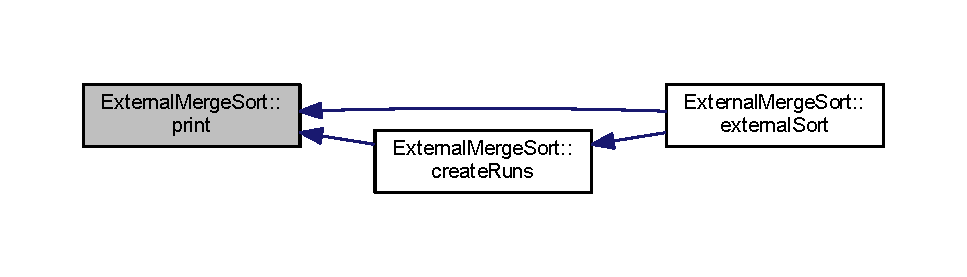
\includegraphics[width=350pt]{class_external_merge_sort_a7a6b94fff35130ed6a498f9a31d0f863_icgraph}
\end{center}
\end{figure}
\hypertarget{class_external_merge_sort_ac0eeaba67ee0703acf73a8a5bf78ebe1}{}\label{class_external_merge_sort_ac0eeaba67ee0703acf73a8a5bf78ebe1} 
\index{External\+Merge\+Sort@{External\+Merge\+Sort}!set\+Log@{set\+Log}}
\index{set\+Log@{set\+Log}!External\+Merge\+Sort@{External\+Merge\+Sort}}
\subsubsection{\texorpdfstring{set\+Log()}{setLog()}}
{\footnotesize\ttfamily void External\+Merge\+Sort\+::set\+Log (\begin{DoxyParamCaption}\item[{\hyperlink{_structures_8h_af67907baa897e9fb84df0cb89795b87c}{Log\+Type}}]{log }\end{DoxyParamCaption})}



Устанавливает тип логгирования. 


\begin{DoxyParams}[1]{Аргументы}
\mbox{\tt in}  & {\em log} & Тип логгирования.\\
\hline
\end{DoxyParams}
Задает тип логгирования\+: With\+Out -\/ без логгирования, File -\/ логгирование в файл log.\+txt, C\+LI -\/ логгирование в консоль. \hypertarget{class_external_merge_sort_a2a27571acdf4f42e34798663e37f5e0b}{}\label{class_external_merge_sort_a2a27571acdf4f42e34798663e37f5e0b} 
\index{External\+Merge\+Sort@{External\+Merge\+Sort}!set\+Params@{set\+Params}}
\index{set\+Params@{set\+Params}!External\+Merge\+Sort@{External\+Merge\+Sort}}
\subsubsection{\texorpdfstring{set\+Params()}{setParams()}}
{\footnotesize\ttfamily \hyperlink{_structures_8h_a9864d6ef28dd6e38416afac4426b3491}{Responce} External\+Merge\+Sort\+::set\+Params (\begin{DoxyParamCaption}\item[{\hyperlink{class_file_manager}{File\+Manager} $\ast$}]{file,  }\item[{long long}]{size\+Of\+Segments }\end{DoxyParamCaption})}



Определение параметров сортировки. 


\begin{DoxyParams}[1]{Аргументы}
\mbox{\tt in}  & {\em file} & Файл-\/менеджер, отвечающий за взаимодействие сортировки с файловой системой. \\
\hline
\mbox{\tt in}  & {\em size\+Of\+Segments} & Размер сегментов. \\
\hline
\end{DoxyParams}
\begin{DoxyReturn}{Возвращает}
Код успеха или ошибки.
\end{DoxyReturn}
Задает параметры сортировки, если это возможно. Устанавливает ok в true или возвращает код ошибки. Возвращает код успеха или ошибки. Граф вызовов\+:\nopagebreak
\begin{figure}[H]
\begin{center}
\leavevmode
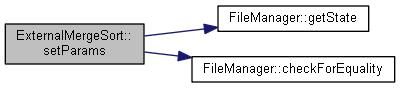
\includegraphics[width=350pt]{class_external_merge_sort_a2a27571acdf4f42e34798663e37f5e0b_cgraph}
\end{center}
\end{figure}
Граф вызова функции\+:\nopagebreak
\begin{figure}[H]
\begin{center}
\leavevmode
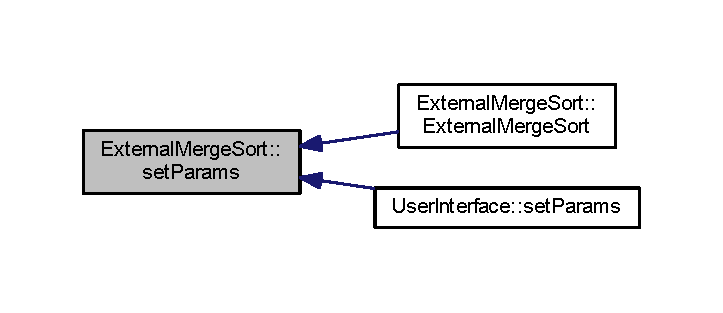
\includegraphics[width=347pt]{class_external_merge_sort_a2a27571acdf4f42e34798663e37f5e0b_icgraph}
\end{center}
\end{figure}
\hypertarget{class_external_merge_sort_a7b777f22151fdd869624d8aa5a39a7bb}{}\label{class_external_merge_sort_a7b777f22151fdd869624d8aa5a39a7bb} 
\index{External\+Merge\+Sort@{External\+Merge\+Sort}!sort@{sort}}
\index{sort@{sort}!External\+Merge\+Sort@{External\+Merge\+Sort}}
\subsubsection{\texorpdfstring{sort()}{sort()}}
{\footnotesize\ttfamily virtual void External\+Merge\+Sort\+::sort (\begin{DoxyParamCaption}\item[{long long $\ast$}]{arr,  }\item[{long long}]{size }\end{DoxyParamCaption})\hspace{0.3cm}{\ttfamily [protected]}, {\ttfamily [pure virtual]}}



Сортирует последовательность длиной size одним из методов, перегруженных в производных классах. 


\begin{DoxyParams}[1]{Аргументы}
\mbox{\tt in}  & {\em arr} & Массив, который необходимо отсортировать. \\
\hline
\mbox{\tt in}  & {\em size} & Длина массива.\\
\hline
\end{DoxyParams}
Чисто виртуальный метод. Перегружен в производных классах. Сортирует последовательность длиной size одним из методов, перегруженных в производных классах. 

Замещается в \hyperlink{class_heap_external_sort_a908087ce13932b268a35e1184a05ea44}{Heap\+External\+Sort}, \hyperlink{class_quick_external_sort_ab277b5945ac22cdcda10bf02e56eb8db}{Quick\+External\+Sort} и \hyperlink{class_bubble_external_sort_a785502521871c44e6d9585108e4254bd}{Bubble\+External\+Sort}.

Граф вызова функции\+:\nopagebreak
\begin{figure}[H]
\begin{center}
\leavevmode
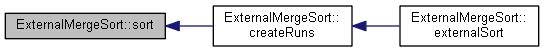
\includegraphics[width=350pt]{class_external_merge_sort_a7b777f22151fdd869624d8aa5a39a7bb_icgraph}
\end{center}
\end{figure}


\subsection{Данные класса}
\hypertarget{class_external_merge_sort_ac9cb039a5cda56e66aecbc17465dd237}{}\label{class_external_merge_sort_ac9cb039a5cda56e66aecbc17465dd237} 
\index{External\+Merge\+Sort@{External\+Merge\+Sort}!counter@{counter}}
\index{counter@{counter}!External\+Merge\+Sort@{External\+Merge\+Sort}}
\subsubsection{\texorpdfstring{counter}{counter}}
{\footnotesize\ttfamily \hyperlink{class_counter}{Counter} External\+Merge\+Sort\+::counter}



Счетчик. 

Счетчик сортировки, подсчитывает характеристики сортировки. \hypertarget{class_external_merge_sort_ab82d3b62a57be6c80dbd12b90de278e2}{}\label{class_external_merge_sort_ab82d3b62a57be6c80dbd12b90de278e2} 
\index{External\+Merge\+Sort@{External\+Merge\+Sort}!file\+Manager@{file\+Manager}}
\index{file\+Manager@{file\+Manager}!External\+Merge\+Sort@{External\+Merge\+Sort}}
\subsubsection{\texorpdfstring{file\+Manager}{fileManager}}
{\footnotesize\ttfamily \hyperlink{class_file_manager}{File\+Manager}$\ast$ External\+Merge\+Sort\+::file\+Manager\hspace{0.3cm}{\ttfamily [private]}}



Указатель на класс файл-\/менеджера. 

Указатель на класс файл-\/менеджера, осуществляющий взаимодействие сортировки с файловой системой. \hypertarget{class_external_merge_sort_a41f61c3beb7dc529d7f2a8b2b4ee380b}{}\label{class_external_merge_sort_a41f61c3beb7dc529d7f2a8b2b4ee380b} 
\index{External\+Merge\+Sort@{External\+Merge\+Sort}!log@{log}}
\index{log@{log}!External\+Merge\+Sort@{External\+Merge\+Sort}}
\subsubsection{\texorpdfstring{log}{log}}
{\footnotesize\ttfamily \hyperlink{_structures_8h_af67907baa897e9fb84df0cb89795b87c}{Log\+Type} External\+Merge\+Sort\+::log\hspace{0.3cm}{\ttfamily [private]}}



Тип логгирования. 

Without -\/ логгирование не ведется, File -\/ логгирование ведется в файл, C\+LI -\/ логгирование ведется в консоль. \hypertarget{class_external_merge_sort_a4b050cd230e144a11f65e57523e15ce6}{}\label{class_external_merge_sort_a4b050cd230e144a11f65e57523e15ce6} 
\index{External\+Merge\+Sort@{External\+Merge\+Sort}!ok@{ok}}
\index{ok@{ok}!External\+Merge\+Sort@{External\+Merge\+Sort}}
\subsubsection{\texorpdfstring{ok}{ok}}
{\footnotesize\ttfamily bool External\+Merge\+Sort\+::ok\hspace{0.3cm}{\ttfamily [private]}}



Флаг готовности сортировки. 

Флаг установлен в true, если все параметры заданы корректно и false, если нет. \hypertarget{class_external_merge_sort_a1d68bb5e0373cf16807a41272dff1a99}{}\label{class_external_merge_sort_a1d68bb5e0373cf16807a41272dff1a99} 
\index{External\+Merge\+Sort@{External\+Merge\+Sort}!size\+Of\+Segments@{size\+Of\+Segments}}
\index{size\+Of\+Segments@{size\+Of\+Segments}!External\+Merge\+Sort@{External\+Merge\+Sort}}
\subsubsection{\texorpdfstring{size\+Of\+Segments}{sizeOfSegments}}
{\footnotesize\ttfamily long long External\+Merge\+Sort\+::size\+Of\+Segments\hspace{0.3cm}{\ttfamily [private]}}



Размер сегментов. 

Размер сегментов, на которые изначально будет поделена последовательность. 

Объявления и описания членов классов находятся в файлах\+:\begin{DoxyCompactItemize}
\item 
C\+:/\+Users/админ/\+Documents/\+Projects\+C++/\+External\+Merge\+Sort\+Production/\+External\+Merge\+Sort\+Production/\hyperlink{_external_merge_sort_8h}{External\+Merge\+Sort.\+h}\item 
C\+:/\+Users/админ/\+Documents/\+Projects\+C++/\+External\+Merge\+Sort\+Production/\+External\+Merge\+Sort\+Production/\hyperlink{_external_merge_sort_8cpp}{External\+Merge\+Sort.\+cpp}\end{DoxyCompactItemize}

\hypertarget{class_file_manager}{}\section{Класс File\+Manager}
\label{class_file_manager}\index{File\+Manager@{File\+Manager}}


{\ttfamily \#include $<$File\+Manager.\+h$>$}



Граф связей класса File\+Manager\+:\nopagebreak
\begin{figure}[H]
\begin{center}
\leavevmode
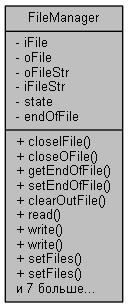
\includegraphics[width=168pt]{class_file_manager__coll__graph}
\end{center}
\end{figure}
\subsection*{Открытые члены}
\begin{DoxyCompactItemize}
\item 
void \hyperlink{class_file_manager_a4a4719a410ca31985e8b75ad75485ce6}{close\+I\+File} ()
\item 
void \hyperlink{class_file_manager_a6a1f1ddbf047fc7e9531f483e4c62148}{close\+O\+File} ()
\item 
bool \hyperlink{class_file_manager_a49df99509ff2700e0e5edd06adca345c}{get\+End\+Of\+File} ()
\item 
void \hyperlink{class_file_manager_ace8ce2677414831b5a9e7030248fc832}{set\+End\+Of\+File} (bool b)
\item 
void \hyperlink{class_file_manager_a2f1102abfd0a5a9d7e178968a3fdc56c}{clear\+Out\+File} ()
\item 
\hyperlink{_structures_8h_a9864d6ef28dd6e38416afac4426b3491}{Responce} \hyperlink{class_file_manager_aba031d681752c80f52a8a8af9b69834e}{read} (long long $\ast$arr, long long size, long long $\ast$read\+Number)
\item 
\hyperlink{_structures_8h_a9864d6ef28dd6e38416afac4426b3491}{Responce} \hyperlink{class_file_manager_a77cb9ec2885923dd6b7a9674cb75f85f}{write} (long long num)
\item 
\hyperlink{_structures_8h_a9864d6ef28dd6e38416afac4426b3491}{Responce} \hyperlink{class_file_manager_ad4c96727180b0055942d20b7b5bfe5f8}{write} (long long $\ast$arr, long long size)
\item 
\hyperlink{_structures_8h_a9864d6ef28dd6e38416afac4426b3491}{Responce} \hyperlink{class_file_manager_ab364b91193c482fc7387aec162f677ad}{set\+Files} (string file, \hyperlink{_structures_8h_a57306ae0f9e356347388234ed69e0ce7}{File\+State} st)
\item 
\hyperlink{_structures_8h_a9864d6ef28dd6e38416afac4426b3491}{Responce} \hyperlink{class_file_manager_a975bf0088fa67c83d78ec54b9f61a473}{set\+Files} (string in\+File, string out\+File)
\item 
\hyperlink{_structures_8h_a57306ae0f9e356347388234ed69e0ce7}{File\+State} \hyperlink{class_file_manager_abd4cbc2b218ab1828ae376a4a9137057}{get\+State} ()
\item 
bool \hyperlink{class_file_manager_ab490a5a5882d33781dcb6d1d42945d97}{check\+For\+Equality} ()
\item 
\hyperlink{_structures_8h_a9864d6ef28dd6e38416afac4426b3491}{Responce} \hyperlink{class_file_manager_a654c8bf606626cd419f5828839cb21a1}{generate\+Sequence} (long long size, \hyperlink{_structures_8h_a76639e910448c3333d0f4d204e53c2c1}{Seq\+Type} type)
\item 
\hyperlink{class_file_manager_a62d69473c95f8df25e44d2466bb00dc5}{File\+Manager} (string \hyperlink{class_file_manager_a91fd33cbb230ed4974a678302e906a8d}{i\+File}, \hyperlink{_structures_8h_a57306ae0f9e356347388234ed69e0ce7}{File\+State} \hyperlink{class_file_manager_a84bbcd4e3807e076ecdbd0e5dfbefa5f}{state})
\item 
\hyperlink{class_file_manager_a2456e56bdcb617c3ee75521cf9dd7057}{File\+Manager} (string in\+File, string out\+File)
\item 
\hyperlink{class_file_manager_a8afd512c06be9daf140cc19d71f9b391}{File\+Manager} ()
\item 
\hyperlink{class_file_manager_abaed33b5b0c13b8a597db9335a1aacfa}{$\sim$\+File\+Manager} ()
\end{DoxyCompactItemize}
\subsection*{Закрытые данные}
\begin{DoxyCompactItemize}
\item 
ifstream $\ast$ \hyperlink{class_file_manager_a91fd33cbb230ed4974a678302e906a8d}{i\+File}
\item 
ofstream $\ast$ \hyperlink{class_file_manager_afe31c07e311212814e4a8ba01c7436a1}{o\+File}
\item 
string $\ast$ \hyperlink{class_file_manager_adf10708d6e8e3b4d329077af4666e147}{o\+File\+Str}
\item 
string $\ast$ \hyperlink{class_file_manager_aaa0e6feed45b6a92ce5c0b509bd9ceb6}{i\+File\+Str}
\item 
\hyperlink{_structures_8h_a57306ae0f9e356347388234ed69e0ce7}{File\+State} \hyperlink{class_file_manager_a84bbcd4e3807e076ecdbd0e5dfbefa5f}{state}
\item 
bool \hyperlink{class_file_manager_ae43001594f1ee182581741d2530620a8}{end\+Of\+File}
\end{DoxyCompactItemize}


\subsection{Конструктор(ы)}
\hypertarget{class_file_manager_a62d69473c95f8df25e44d2466bb00dc5}{}\label{class_file_manager_a62d69473c95f8df25e44d2466bb00dc5} 
\index{File\+Manager@{File\+Manager}!File\+Manager@{File\+Manager}}
\index{File\+Manager@{File\+Manager}!File\+Manager@{File\+Manager}}
\subsubsection{\texorpdfstring{File\+Manager()}{FileManager()}\hspace{0.1cm}{\footnotesize\ttfamily [1/3]}}
{\footnotesize\ttfamily File\+Manager\+::\+File\+Manager (\begin{DoxyParamCaption}\item[{string}]{i\+File,  }\item[{\hyperlink{_structures_8h_a57306ae0f9e356347388234ed69e0ce7}{File\+State}}]{state }\end{DoxyParamCaption})}

\hypertarget{class_file_manager_a2456e56bdcb617c3ee75521cf9dd7057}{}\label{class_file_manager_a2456e56bdcb617c3ee75521cf9dd7057} 
\index{File\+Manager@{File\+Manager}!File\+Manager@{File\+Manager}}
\index{File\+Manager@{File\+Manager}!File\+Manager@{File\+Manager}}
\subsubsection{\texorpdfstring{File\+Manager()}{FileManager()}\hspace{0.1cm}{\footnotesize\ttfamily [2/3]}}
{\footnotesize\ttfamily File\+Manager\+::\+File\+Manager (\begin{DoxyParamCaption}\item[{string}]{in\+File,  }\item[{string}]{out\+File }\end{DoxyParamCaption})}

\hypertarget{class_file_manager_a8afd512c06be9daf140cc19d71f9b391}{}\label{class_file_manager_a8afd512c06be9daf140cc19d71f9b391} 
\index{File\+Manager@{File\+Manager}!File\+Manager@{File\+Manager}}
\index{File\+Manager@{File\+Manager}!File\+Manager@{File\+Manager}}
\subsubsection{\texorpdfstring{File\+Manager()}{FileManager()}\hspace{0.1cm}{\footnotesize\ttfamily [3/3]}}
{\footnotesize\ttfamily File\+Manager\+::\+File\+Manager (\begin{DoxyParamCaption}{ }\end{DoxyParamCaption})}

\hypertarget{class_file_manager_abaed33b5b0c13b8a597db9335a1aacfa}{}\label{class_file_manager_abaed33b5b0c13b8a597db9335a1aacfa} 
\index{File\+Manager@{File\+Manager}!````~File\+Manager@{$\sim$\+File\+Manager}}
\index{````~File\+Manager@{$\sim$\+File\+Manager}!File\+Manager@{File\+Manager}}
\subsubsection{\texorpdfstring{$\sim$\+File\+Manager()}{~FileManager()}}
{\footnotesize\ttfamily File\+Manager\+::$\sim$\+File\+Manager (\begin{DoxyParamCaption}{ }\end{DoxyParamCaption})}



\subsection{Методы}
\hypertarget{class_file_manager_ab490a5a5882d33781dcb6d1d42945d97}{}\label{class_file_manager_ab490a5a5882d33781dcb6d1d42945d97} 
\index{File\+Manager@{File\+Manager}!check\+For\+Equality@{check\+For\+Equality}}
\index{check\+For\+Equality@{check\+For\+Equality}!File\+Manager@{File\+Manager}}
\subsubsection{\texorpdfstring{check\+For\+Equality()}{checkForEquality()}}
{\footnotesize\ttfamily bool File\+Manager\+::check\+For\+Equality (\begin{DoxyParamCaption}{ }\end{DoxyParamCaption})}

Граф вызова функции\+:\nopagebreak
\begin{figure}[H]
\begin{center}
\leavevmode
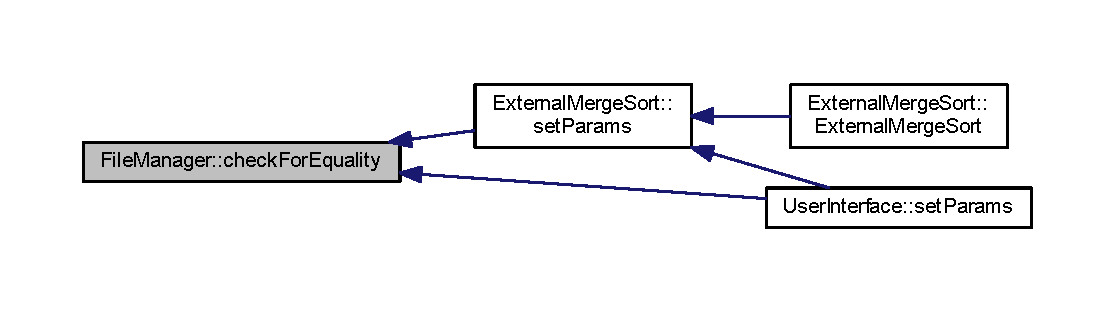
\includegraphics[width=350pt]{class_file_manager_ab490a5a5882d33781dcb6d1d42945d97_icgraph}
\end{center}
\end{figure}
\hypertarget{class_file_manager_a2f1102abfd0a5a9d7e178968a3fdc56c}{}\label{class_file_manager_a2f1102abfd0a5a9d7e178968a3fdc56c} 
\index{File\+Manager@{File\+Manager}!clear\+Out\+File@{clear\+Out\+File}}
\index{clear\+Out\+File@{clear\+Out\+File}!File\+Manager@{File\+Manager}}
\subsubsection{\texorpdfstring{clear\+Out\+File()}{clearOutFile()}}
{\footnotesize\ttfamily void File\+Manager\+::clear\+Out\+File (\begin{DoxyParamCaption}{ }\end{DoxyParamCaption})}

Граф вызова функции\+:\nopagebreak
\begin{figure}[H]
\begin{center}
\leavevmode
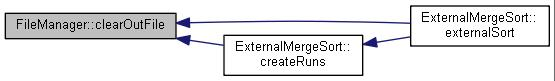
\includegraphics[width=350pt]{class_file_manager_a2f1102abfd0a5a9d7e178968a3fdc56c_icgraph}
\end{center}
\end{figure}
\hypertarget{class_file_manager_a4a4719a410ca31985e8b75ad75485ce6}{}\label{class_file_manager_a4a4719a410ca31985e8b75ad75485ce6} 
\index{File\+Manager@{File\+Manager}!close\+I\+File@{close\+I\+File}}
\index{close\+I\+File@{close\+I\+File}!File\+Manager@{File\+Manager}}
\subsubsection{\texorpdfstring{close\+I\+File()}{closeIFile()}}
{\footnotesize\ttfamily void File\+Manager\+::close\+I\+File (\begin{DoxyParamCaption}{ }\end{DoxyParamCaption})}

Граф вызова функции\+:\nopagebreak
\begin{figure}[H]
\begin{center}
\leavevmode
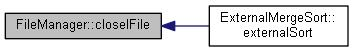
\includegraphics[width=337pt]{class_file_manager_a4a4719a410ca31985e8b75ad75485ce6_icgraph}
\end{center}
\end{figure}
\hypertarget{class_file_manager_a6a1f1ddbf047fc7e9531f483e4c62148}{}\label{class_file_manager_a6a1f1ddbf047fc7e9531f483e4c62148} 
\index{File\+Manager@{File\+Manager}!close\+O\+File@{close\+O\+File}}
\index{close\+O\+File@{close\+O\+File}!File\+Manager@{File\+Manager}}
\subsubsection{\texorpdfstring{close\+O\+File()}{closeOFile()}}
{\footnotesize\ttfamily void File\+Manager\+::close\+O\+File (\begin{DoxyParamCaption}{ }\end{DoxyParamCaption})}

Граф вызова функции\+:\nopagebreak
\begin{figure}[H]
\begin{center}
\leavevmode
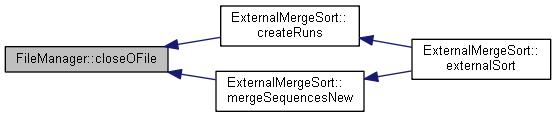
\includegraphics[width=350pt]{class_file_manager_a6a1f1ddbf047fc7e9531f483e4c62148_icgraph}
\end{center}
\end{figure}
\hypertarget{class_file_manager_a654c8bf606626cd419f5828839cb21a1}{}\label{class_file_manager_a654c8bf606626cd419f5828839cb21a1} 
\index{File\+Manager@{File\+Manager}!generate\+Sequence@{generate\+Sequence}}
\index{generate\+Sequence@{generate\+Sequence}!File\+Manager@{File\+Manager}}
\subsubsection{\texorpdfstring{generate\+Sequence()}{generateSequence()}}
{\footnotesize\ttfamily \hyperlink{_structures_8h_a9864d6ef28dd6e38416afac4426b3491}{Responce} File\+Manager\+::generate\+Sequence (\begin{DoxyParamCaption}\item[{long long}]{size,  }\item[{\hyperlink{_structures_8h_a76639e910448c3333d0f4d204e53c2c1}{Seq\+Type}}]{type }\end{DoxyParamCaption})}

Граф вызова функции\+:\nopagebreak
\begin{figure}[H]
\begin{center}
\leavevmode
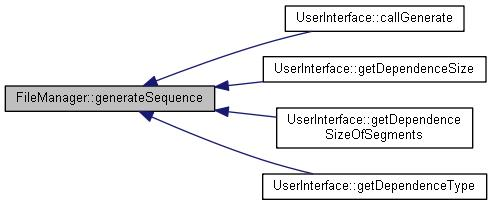
\includegraphics[width=350pt]{class_file_manager_a654c8bf606626cd419f5828839cb21a1_icgraph}
\end{center}
\end{figure}
\hypertarget{class_file_manager_a49df99509ff2700e0e5edd06adca345c}{}\label{class_file_manager_a49df99509ff2700e0e5edd06adca345c} 
\index{File\+Manager@{File\+Manager}!get\+End\+Of\+File@{get\+End\+Of\+File}}
\index{get\+End\+Of\+File@{get\+End\+Of\+File}!File\+Manager@{File\+Manager}}
\subsubsection{\texorpdfstring{get\+End\+Of\+File()}{getEndOfFile()}}
{\footnotesize\ttfamily bool File\+Manager\+::get\+End\+Of\+File (\begin{DoxyParamCaption}{ }\end{DoxyParamCaption})}

Граф вызова функции\+:\nopagebreak
\begin{figure}[H]
\begin{center}
\leavevmode
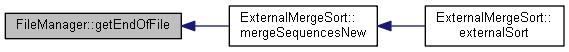
\includegraphics[width=350pt]{class_file_manager_a49df99509ff2700e0e5edd06adca345c_icgraph}
\end{center}
\end{figure}
\hypertarget{class_file_manager_abd4cbc2b218ab1828ae376a4a9137057}{}\label{class_file_manager_abd4cbc2b218ab1828ae376a4a9137057} 
\index{File\+Manager@{File\+Manager}!get\+State@{get\+State}}
\index{get\+State@{get\+State}!File\+Manager@{File\+Manager}}
\subsubsection{\texorpdfstring{get\+State()}{getState()}}
{\footnotesize\ttfamily \hyperlink{_structures_8h_a57306ae0f9e356347388234ed69e0ce7}{File\+State} File\+Manager\+::get\+State (\begin{DoxyParamCaption}{ }\end{DoxyParamCaption})}

Граф вызова функции\+:\nopagebreak
\begin{figure}[H]
\begin{center}
\leavevmode
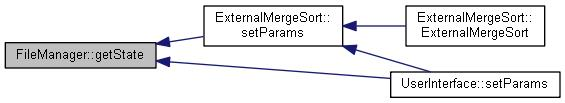
\includegraphics[width=350pt]{class_file_manager_abd4cbc2b218ab1828ae376a4a9137057_icgraph}
\end{center}
\end{figure}
\hypertarget{class_file_manager_aba031d681752c80f52a8a8af9b69834e}{}\label{class_file_manager_aba031d681752c80f52a8a8af9b69834e} 
\index{File\+Manager@{File\+Manager}!read@{read}}
\index{read@{read}!File\+Manager@{File\+Manager}}
\subsubsection{\texorpdfstring{read()}{read()}}
{\footnotesize\ttfamily \hyperlink{_structures_8h_a9864d6ef28dd6e38416afac4426b3491}{Responce} File\+Manager\+::read (\begin{DoxyParamCaption}\item[{long long $\ast$}]{arr,  }\item[{long long}]{size,  }\item[{long long $\ast$}]{read\+Number }\end{DoxyParamCaption})}

Граф вызова функции\+:\nopagebreak
\begin{figure}[H]
\begin{center}
\leavevmode
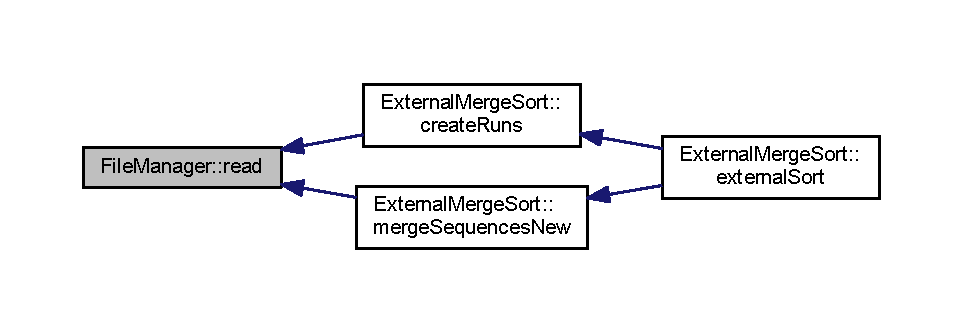
\includegraphics[width=350pt]{class_file_manager_aba031d681752c80f52a8a8af9b69834e_icgraph}
\end{center}
\end{figure}
\hypertarget{class_file_manager_ace8ce2677414831b5a9e7030248fc832}{}\label{class_file_manager_ace8ce2677414831b5a9e7030248fc832} 
\index{File\+Manager@{File\+Manager}!set\+End\+Of\+File@{set\+End\+Of\+File}}
\index{set\+End\+Of\+File@{set\+End\+Of\+File}!File\+Manager@{File\+Manager}}
\subsubsection{\texorpdfstring{set\+End\+Of\+File()}{setEndOfFile()}}
{\footnotesize\ttfamily void File\+Manager\+::set\+End\+Of\+File (\begin{DoxyParamCaption}\item[{bool}]{b }\end{DoxyParamCaption})}

Граф вызова функции\+:\nopagebreak
\begin{figure}[H]
\begin{center}
\leavevmode
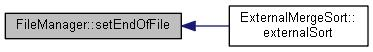
\includegraphics[width=350pt]{class_file_manager_ace8ce2677414831b5a9e7030248fc832_icgraph}
\end{center}
\end{figure}
\hypertarget{class_file_manager_ab364b91193c482fc7387aec162f677ad}{}\label{class_file_manager_ab364b91193c482fc7387aec162f677ad} 
\index{File\+Manager@{File\+Manager}!set\+Files@{set\+Files}}
\index{set\+Files@{set\+Files}!File\+Manager@{File\+Manager}}
\subsubsection{\texorpdfstring{set\+Files()}{setFiles()}\hspace{0.1cm}{\footnotesize\ttfamily [1/2]}}
{\footnotesize\ttfamily \hyperlink{_structures_8h_a9864d6ef28dd6e38416afac4426b3491}{Responce} File\+Manager\+::set\+Files (\begin{DoxyParamCaption}\item[{string}]{file,  }\item[{\hyperlink{_structures_8h_a57306ae0f9e356347388234ed69e0ce7}{File\+State}}]{st }\end{DoxyParamCaption})}

\hypertarget{class_file_manager_a975bf0088fa67c83d78ec54b9f61a473}{}\label{class_file_manager_a975bf0088fa67c83d78ec54b9f61a473} 
\index{File\+Manager@{File\+Manager}!set\+Files@{set\+Files}}
\index{set\+Files@{set\+Files}!File\+Manager@{File\+Manager}}
\subsubsection{\texorpdfstring{set\+Files()}{setFiles()}\hspace{0.1cm}{\footnotesize\ttfamily [2/2]}}
{\footnotesize\ttfamily \hyperlink{_structures_8h_a9864d6ef28dd6e38416afac4426b3491}{Responce} File\+Manager\+::set\+Files (\begin{DoxyParamCaption}\item[{string}]{in\+File,  }\item[{string}]{out\+File }\end{DoxyParamCaption})}

\hypertarget{class_file_manager_a77cb9ec2885923dd6b7a9674cb75f85f}{}\label{class_file_manager_a77cb9ec2885923dd6b7a9674cb75f85f} 
\index{File\+Manager@{File\+Manager}!write@{write}}
\index{write@{write}!File\+Manager@{File\+Manager}}
\subsubsection{\texorpdfstring{write()}{write()}\hspace{0.1cm}{\footnotesize\ttfamily [1/2]}}
{\footnotesize\ttfamily \hyperlink{_structures_8h_a9864d6ef28dd6e38416afac4426b3491}{Responce} File\+Manager\+::write (\begin{DoxyParamCaption}\item[{long long}]{num }\end{DoxyParamCaption})}

Граф вызова функции\+:\nopagebreak
\begin{figure}[H]
\begin{center}
\leavevmode
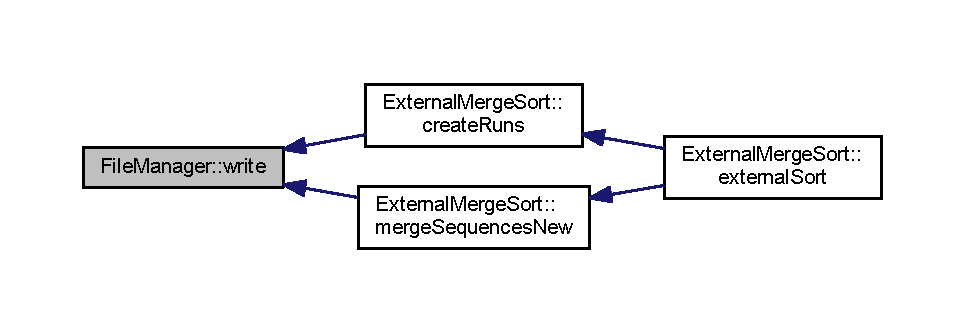
\includegraphics[width=350pt]{class_file_manager_a77cb9ec2885923dd6b7a9674cb75f85f_icgraph}
\end{center}
\end{figure}
\hypertarget{class_file_manager_ad4c96727180b0055942d20b7b5bfe5f8}{}\label{class_file_manager_ad4c96727180b0055942d20b7b5bfe5f8} 
\index{File\+Manager@{File\+Manager}!write@{write}}
\index{write@{write}!File\+Manager@{File\+Manager}}
\subsubsection{\texorpdfstring{write()}{write()}\hspace{0.1cm}{\footnotesize\ttfamily [2/2]}}
{\footnotesize\ttfamily \hyperlink{_structures_8h_a9864d6ef28dd6e38416afac4426b3491}{Responce} File\+Manager\+::write (\begin{DoxyParamCaption}\item[{long long $\ast$}]{arr,  }\item[{long long}]{size }\end{DoxyParamCaption})}



\subsection{Данные класса}
\hypertarget{class_file_manager_ae43001594f1ee182581741d2530620a8}{}\label{class_file_manager_ae43001594f1ee182581741d2530620a8} 
\index{File\+Manager@{File\+Manager}!end\+Of\+File@{end\+Of\+File}}
\index{end\+Of\+File@{end\+Of\+File}!File\+Manager@{File\+Manager}}
\subsubsection{\texorpdfstring{end\+Of\+File}{endOfFile}}
{\footnotesize\ttfamily bool File\+Manager\+::end\+Of\+File\hspace{0.3cm}{\ttfamily [private]}}

\hypertarget{class_file_manager_a91fd33cbb230ed4974a678302e906a8d}{}\label{class_file_manager_a91fd33cbb230ed4974a678302e906a8d} 
\index{File\+Manager@{File\+Manager}!i\+File@{i\+File}}
\index{i\+File@{i\+File}!File\+Manager@{File\+Manager}}
\subsubsection{\texorpdfstring{i\+File}{iFile}}
{\footnotesize\ttfamily ifstream$\ast$ File\+Manager\+::i\+File\hspace{0.3cm}{\ttfamily [private]}}

\hypertarget{class_file_manager_aaa0e6feed45b6a92ce5c0b509bd9ceb6}{}\label{class_file_manager_aaa0e6feed45b6a92ce5c0b509bd9ceb6} 
\index{File\+Manager@{File\+Manager}!i\+File\+Str@{i\+File\+Str}}
\index{i\+File\+Str@{i\+File\+Str}!File\+Manager@{File\+Manager}}
\subsubsection{\texorpdfstring{i\+File\+Str}{iFileStr}}
{\footnotesize\ttfamily string$\ast$ File\+Manager\+::i\+File\+Str\hspace{0.3cm}{\ttfamily [private]}}

\hypertarget{class_file_manager_afe31c07e311212814e4a8ba01c7436a1}{}\label{class_file_manager_afe31c07e311212814e4a8ba01c7436a1} 
\index{File\+Manager@{File\+Manager}!o\+File@{o\+File}}
\index{o\+File@{o\+File}!File\+Manager@{File\+Manager}}
\subsubsection{\texorpdfstring{o\+File}{oFile}}
{\footnotesize\ttfamily ofstream$\ast$ File\+Manager\+::o\+File\hspace{0.3cm}{\ttfamily [private]}}

\hypertarget{class_file_manager_adf10708d6e8e3b4d329077af4666e147}{}\label{class_file_manager_adf10708d6e8e3b4d329077af4666e147} 
\index{File\+Manager@{File\+Manager}!o\+File\+Str@{o\+File\+Str}}
\index{o\+File\+Str@{o\+File\+Str}!File\+Manager@{File\+Manager}}
\subsubsection{\texorpdfstring{o\+File\+Str}{oFileStr}}
{\footnotesize\ttfamily string$\ast$ File\+Manager\+::o\+File\+Str\hspace{0.3cm}{\ttfamily [private]}}

\hypertarget{class_file_manager_a84bbcd4e3807e076ecdbd0e5dfbefa5f}{}\label{class_file_manager_a84bbcd4e3807e076ecdbd0e5dfbefa5f} 
\index{File\+Manager@{File\+Manager}!state@{state}}
\index{state@{state}!File\+Manager@{File\+Manager}}
\subsubsection{\texorpdfstring{state}{state}}
{\footnotesize\ttfamily \hyperlink{_structures_8h_a57306ae0f9e356347388234ed69e0ce7}{File\+State} File\+Manager\+::state\hspace{0.3cm}{\ttfamily [private]}}



Объявления и описания членов классов находятся в файлах\+:\begin{DoxyCompactItemize}
\item 
C\+:/\+Users/админ/\+Documents/\+Projects\+C++/\+External\+Merge\+Sort\+Production/\+External\+Merge\+Sort\+Production/\hyperlink{_file_manager_8h}{File\+Manager.\+h}\item 
C\+:/\+Users/админ/\+Documents/\+Projects\+C++/\+External\+Merge\+Sort\+Production/\+External\+Merge\+Sort\+Production/\hyperlink{_file_manager_8cpp}{File\+Manager.\+cpp}\end{DoxyCompactItemize}

\hypertarget{class_heap_external_sort}{}\section{Класс Heap\+External\+Sort}
\label{class_heap_external_sort}\index{Heap\+External\+Sort@{Heap\+External\+Sort}}


{\ttfamily \#include $<$Heap\+External\+Sort.\+h$>$}



Граф наследования\+:Heap\+External\+Sort\+:\nopagebreak
\begin{figure}[H]
\begin{center}
\leavevmode
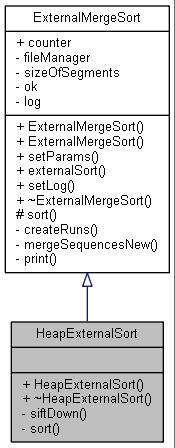
\includegraphics[width=203pt]{class_heap_external_sort__inherit__graph}
\end{center}
\end{figure}


Граф связей класса Heap\+External\+Sort\+:\nopagebreak
\begin{figure}[H]
\begin{center}
\leavevmode
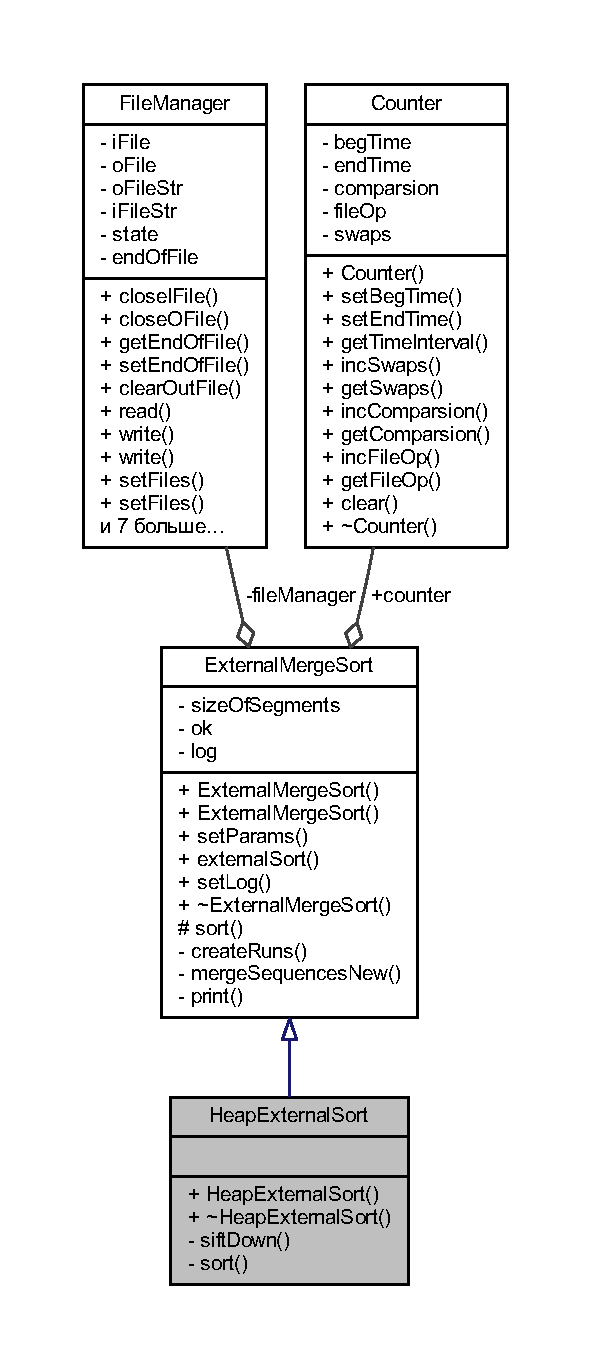
\includegraphics[height=550pt]{class_heap_external_sort__coll__graph}
\end{center}
\end{figure}
\subsection*{Открытые члены}
\begin{DoxyCompactItemize}
\item 
virtual void \hyperlink{class_heap_external_sort_a908087ce13932b268a35e1184a05ea44}{sort} (long long $\ast$numbers, long long array\+\_\+size)
\item 
\hyperlink{class_heap_external_sort_a9e6236e47430f0b530b287a6d7cf3a8b}{Heap\+External\+Sort} ()
\item 
\hyperlink{class_heap_external_sort_afa76473510a8cb610bb94bca5b5202c9}{$\sim$\+Heap\+External\+Sort} ()
\end{DoxyCompactItemize}
\subsection*{Закрытые члены}
\begin{DoxyCompactItemize}
\item 
void \hyperlink{class_heap_external_sort_a927eea9dcf44a9c7d53db1039bc7e21f}{sift\+Down} (long long $\ast$numbers, long long root, long long bottom)
\end{DoxyCompactItemize}
\subsection*{Дополнительные унаследованные члены}


\subsection{Конструктор(ы)}
\hypertarget{class_heap_external_sort_a9e6236e47430f0b530b287a6d7cf3a8b}{}\label{class_heap_external_sort_a9e6236e47430f0b530b287a6d7cf3a8b} 
\index{Heap\+External\+Sort@{Heap\+External\+Sort}!Heap\+External\+Sort@{Heap\+External\+Sort}}
\index{Heap\+External\+Sort@{Heap\+External\+Sort}!Heap\+External\+Sort@{Heap\+External\+Sort}}
\subsubsection{\texorpdfstring{Heap\+External\+Sort()}{HeapExternalSort()}}
{\footnotesize\ttfamily Heap\+External\+Sort\+::\+Heap\+External\+Sort (\begin{DoxyParamCaption}{ }\end{DoxyParamCaption})}

\hypertarget{class_heap_external_sort_afa76473510a8cb610bb94bca5b5202c9}{}\label{class_heap_external_sort_afa76473510a8cb610bb94bca5b5202c9} 
\index{Heap\+External\+Sort@{Heap\+External\+Sort}!````~Heap\+External\+Sort@{$\sim$\+Heap\+External\+Sort}}
\index{````~Heap\+External\+Sort@{$\sim$\+Heap\+External\+Sort}!Heap\+External\+Sort@{Heap\+External\+Sort}}
\subsubsection{\texorpdfstring{$\sim$\+Heap\+External\+Sort()}{~HeapExternalSort()}}
{\footnotesize\ttfamily Heap\+External\+Sort\+::$\sim$\+Heap\+External\+Sort (\begin{DoxyParamCaption}{ }\end{DoxyParamCaption})}



\subsection{Методы}
\hypertarget{class_heap_external_sort_a927eea9dcf44a9c7d53db1039bc7e21f}{}\label{class_heap_external_sort_a927eea9dcf44a9c7d53db1039bc7e21f} 
\index{Heap\+External\+Sort@{Heap\+External\+Sort}!sift\+Down@{sift\+Down}}
\index{sift\+Down@{sift\+Down}!Heap\+External\+Sort@{Heap\+External\+Sort}}
\subsubsection{\texorpdfstring{sift\+Down()}{siftDown()}}
{\footnotesize\ttfamily void Heap\+External\+Sort\+::sift\+Down (\begin{DoxyParamCaption}\item[{long long $\ast$}]{numbers,  }\item[{long long}]{root,  }\item[{long long}]{bottom }\end{DoxyParamCaption})\hspace{0.3cm}{\ttfamily [private]}}

Граф вызовов\+:\nopagebreak
\begin{figure}[H]
\begin{center}
\leavevmode
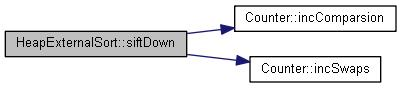
\includegraphics[width=350pt]{class_heap_external_sort_a927eea9dcf44a9c7d53db1039bc7e21f_cgraph}
\end{center}
\end{figure}
Граф вызова функции\+:\nopagebreak
\begin{figure}[H]
\begin{center}
\leavevmode
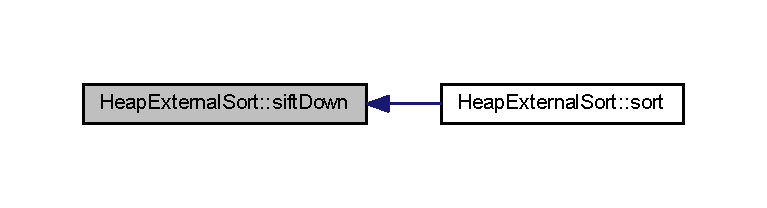
\includegraphics[width=350pt]{class_heap_external_sort_a927eea9dcf44a9c7d53db1039bc7e21f_icgraph}
\end{center}
\end{figure}
\hypertarget{class_heap_external_sort_a908087ce13932b268a35e1184a05ea44}{}\label{class_heap_external_sort_a908087ce13932b268a35e1184a05ea44} 
\index{Heap\+External\+Sort@{Heap\+External\+Sort}!sort@{sort}}
\index{sort@{sort}!Heap\+External\+Sort@{Heap\+External\+Sort}}
\subsubsection{\texorpdfstring{sort()}{sort()}}
{\footnotesize\ttfamily void Heap\+External\+Sort\+::sort (\begin{DoxyParamCaption}\item[{long long $\ast$}]{numbers,  }\item[{long long}]{array\+\_\+size }\end{DoxyParamCaption})\hspace{0.3cm}{\ttfamily [virtual]}}



Замещает \hyperlink{class_external_merge_sort_af6412221cc797a846243a343ccc12dba}{External\+Merge\+Sort}.

Граф вызовов\+:\nopagebreak
\begin{figure}[H]
\begin{center}
\leavevmode
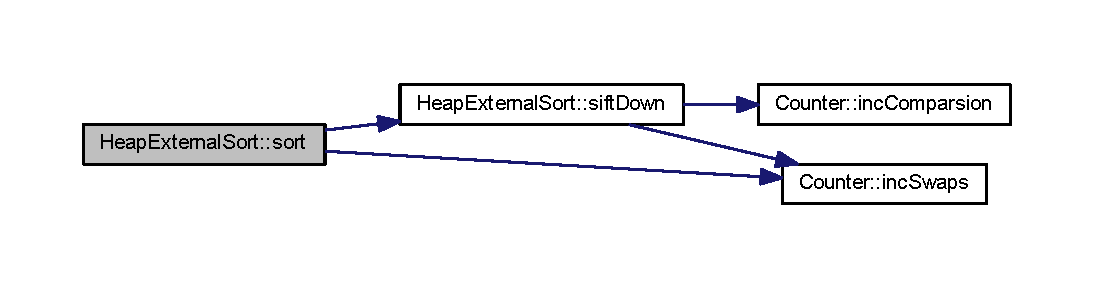
\includegraphics[width=350pt]{class_heap_external_sort_a908087ce13932b268a35e1184a05ea44_cgraph}
\end{center}
\end{figure}


Объявления и описания членов классов находятся в файлах\+:\begin{DoxyCompactItemize}
\item 
C\+:/\+Users/админ/\+Documents/\+Projects\+C++/\+External\+Merge\+Sort\+Production/\+External\+Merge\+Sort\+Production/\hyperlink{_heap_external_sort_8h}{Heap\+External\+Sort.\+h}\item 
C\+:/\+Users/админ/\+Documents/\+Projects\+C++/\+External\+Merge\+Sort\+Production/\+External\+Merge\+Sort\+Production/\hyperlink{_heap_external_sort_8cpp}{Heap\+External\+Sort.\+cpp}\end{DoxyCompactItemize}

\hypertarget{class_quick_external_sort}{}\section{Класс Quick\+External\+Sort}
\label{class_quick_external_sort}\index{Quick\+External\+Sort@{Quick\+External\+Sort}}


\subsection{Подробное описание}
Класс внешней многофазной сортировки слиянием, использующий внутреннюю быструю сортировку. 

\begin{DoxyAuthor}{Автор}
Alexander Filippov 
\end{DoxyAuthor}
\begin{DoxyDate}{Дата}
Ноябрь 2016 года
\end{DoxyDate}
Наследуется от \hyperlink{class_external_merge_sort}{External\+Merge\+Sort}, перегружает метод внутренней сортировки, который осуществляет быструю сортировку последовательности. 

{\ttfamily \#include $<$Quick\+External\+Sort.\+h$>$}



Граф наследования\+:Quick\+External\+Sort\+:\nopagebreak
\begin{figure}[H]
\begin{center}
\leavevmode
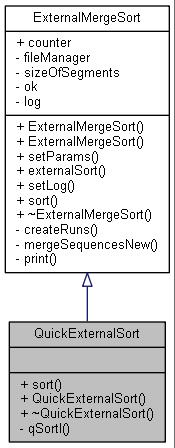
\includegraphics[width=203pt]{class_quick_external_sort__inherit__graph}
\end{center}
\end{figure}


Граф связей класса Quick\+External\+Sort\+:\nopagebreak
\begin{figure}[H]
\begin{center}
\leavevmode
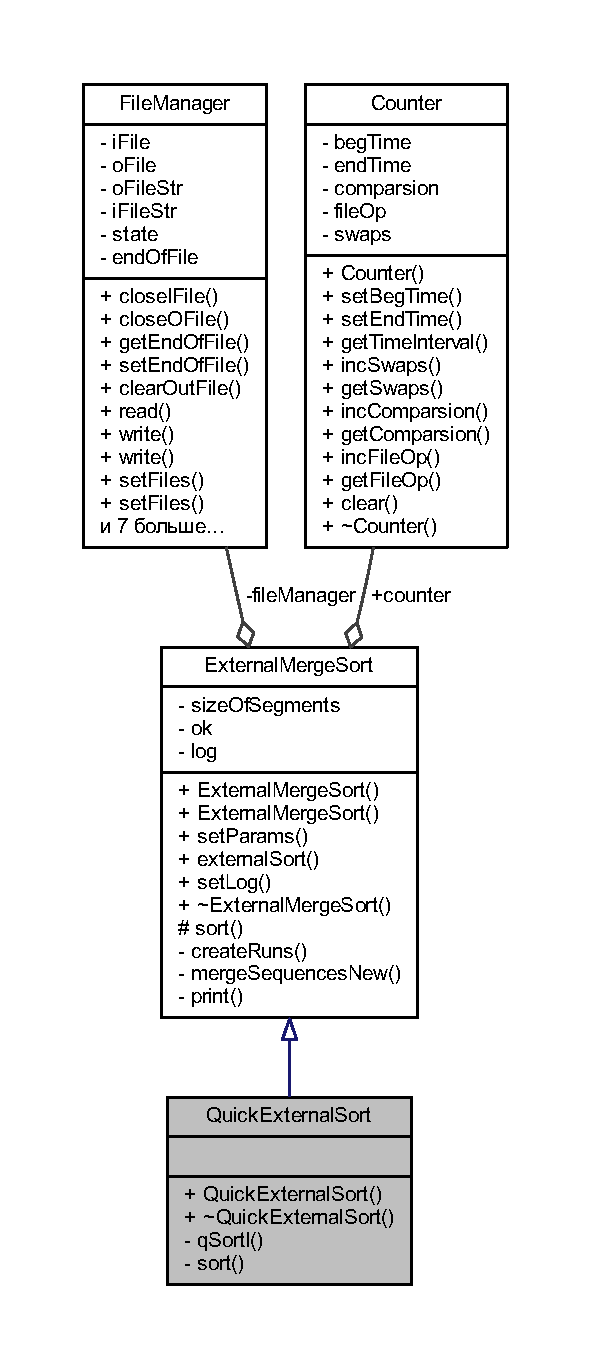
\includegraphics[height=550pt]{class_quick_external_sort__coll__graph}
\end{center}
\end{figure}
\subsection*{Открытые члены}
\begin{DoxyCompactItemize}
\item 
\hyperlink{class_quick_external_sort_ac31914e67af41c48b8fdcbcc076168ed}{Quick\+External\+Sort} ()
\begin{DoxyCompactList}\small\item\em Пустой конструктор класса. \end{DoxyCompactList}\item 
\hyperlink{class_quick_external_sort_a370e2be5e7c4afc31f9b230c2ee4d689}{$\sim$\+Quick\+External\+Sort} ()
\begin{DoxyCompactList}\small\item\em Пустой виртуальный деструктор класса. \end{DoxyCompactList}\end{DoxyCompactItemize}
\subsection*{Закрытые члены}
\begin{DoxyCompactItemize}
\item 
void \hyperlink{class_quick_external_sort_ad7653bb697a04717066f9942db9a4597}{q\+SortI} (long long $\ast$arr, long long size)
\begin{DoxyCompactList}\small\item\em Сортирует последовательность длиной size методом быстрой сортировки итеративным методом. \end{DoxyCompactList}\item 
virtual void \hyperlink{class_quick_external_sort_ab277b5945ac22cdcda10bf02e56eb8db}{sort} (long long $\ast$arr, long long size)
\begin{DoxyCompactList}\small\item\em Сортирует последовательность длиной size методом быстрой сортировки. \end{DoxyCompactList}\end{DoxyCompactItemize}
\subsection*{Дополнительные унаследованные члены}


\subsection{Конструктор(ы)}
\hypertarget{class_quick_external_sort_ac31914e67af41c48b8fdcbcc076168ed}{}\label{class_quick_external_sort_ac31914e67af41c48b8fdcbcc076168ed} 
\index{Quick\+External\+Sort@{Quick\+External\+Sort}!Quick\+External\+Sort@{Quick\+External\+Sort}}
\index{Quick\+External\+Sort@{Quick\+External\+Sort}!Quick\+External\+Sort@{Quick\+External\+Sort}}
\subsubsection{\texorpdfstring{Quick\+External\+Sort()}{QuickExternalSort()}}
{\footnotesize\ttfamily Quick\+External\+Sort\+::\+Quick\+External\+Sort (\begin{DoxyParamCaption}{ }\end{DoxyParamCaption})}



Пустой конструктор класса. 

Обнуляет атрибуты. \hypertarget{class_quick_external_sort_a370e2be5e7c4afc31f9b230c2ee4d689}{}\label{class_quick_external_sort_a370e2be5e7c4afc31f9b230c2ee4d689} 
\index{Quick\+External\+Sort@{Quick\+External\+Sort}!````~Quick\+External\+Sort@{$\sim$\+Quick\+External\+Sort}}
\index{````~Quick\+External\+Sort@{$\sim$\+Quick\+External\+Sort}!Quick\+External\+Sort@{Quick\+External\+Sort}}
\subsubsection{\texorpdfstring{$\sim$\+Quick\+External\+Sort()}{~QuickExternalSort()}}
{\footnotesize\ttfamily Quick\+External\+Sort\+::$\sim$\+Quick\+External\+Sort (\begin{DoxyParamCaption}{ }\end{DoxyParamCaption})}



Пустой виртуальный деструктор класса. 

Освобождает выделенную память. 

\subsection{Методы}
\hypertarget{class_quick_external_sort_ad7653bb697a04717066f9942db9a4597}{}\label{class_quick_external_sort_ad7653bb697a04717066f9942db9a4597} 
\index{Quick\+External\+Sort@{Quick\+External\+Sort}!q\+SortI@{q\+SortI}}
\index{q\+SortI@{q\+SortI}!Quick\+External\+Sort@{Quick\+External\+Sort}}
\subsubsection{\texorpdfstring{q\+Sort\+I()}{qSortI()}}
{\footnotesize\ttfamily void Quick\+External\+Sort\+::q\+SortI (\begin{DoxyParamCaption}\item[{long long $\ast$}]{arr,  }\item[{long long}]{size }\end{DoxyParamCaption})\hspace{0.3cm}{\ttfamily [private]}}



Сортирует последовательность длиной size методом быстрой сортировки итеративным методом. 


\begin{DoxyParams}[1]{Аргументы}
\mbox{\tt in}  & {\em arr} & Массив, который необходимо отсортировать. \\
\hline
\mbox{\tt in}  & {\em size} & Длина массива.\\
\hline
\end{DoxyParams}
Сортирует последовательность длиной size методом быстрой сортировки. Граф вызовов\+:\nopagebreak
\begin{figure}[H]
\begin{center}
\leavevmode
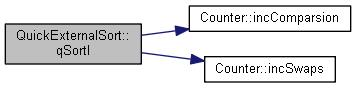
\includegraphics[width=339pt]{class_quick_external_sort_ad7653bb697a04717066f9942db9a4597_cgraph}
\end{center}
\end{figure}
Граф вызова функции\+:\nopagebreak
\begin{figure}[H]
\begin{center}
\leavevmode
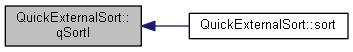
\includegraphics[width=337pt]{class_quick_external_sort_ad7653bb697a04717066f9942db9a4597_icgraph}
\end{center}
\end{figure}
\hypertarget{class_quick_external_sort_ab277b5945ac22cdcda10bf02e56eb8db}{}\label{class_quick_external_sort_ab277b5945ac22cdcda10bf02e56eb8db} 
\index{Quick\+External\+Sort@{Quick\+External\+Sort}!sort@{sort}}
\index{sort@{sort}!Quick\+External\+Sort@{Quick\+External\+Sort}}
\subsubsection{\texorpdfstring{sort()}{sort()}}
{\footnotesize\ttfamily void Quick\+External\+Sort\+::sort (\begin{DoxyParamCaption}\item[{long long $\ast$}]{arr,  }\item[{long long}]{size }\end{DoxyParamCaption})\hspace{0.3cm}{\ttfamily [private]}, {\ttfamily [virtual]}}



Сортирует последовательность длиной size методом быстрой сортировки. 


\begin{DoxyParams}[1]{Аргументы}
\mbox{\tt in}  & {\em arr} & Массив, который необходимо отсортировать. \\
\hline
\mbox{\tt in}  & {\em size} & Длина массива.\\
\hline
\end{DoxyParams}
Виртуальный метод. Перегружен в классе. Вызывет q\+SortI(...), который сортирует последовательность длиной size методом быстрой сортировки. 

Замещает \hyperlink{class_external_merge_sort_a7b777f22151fdd869624d8aa5a39a7bb}{External\+Merge\+Sort}.

Граф вызовов\+:\nopagebreak
\begin{figure}[H]
\begin{center}
\leavevmode
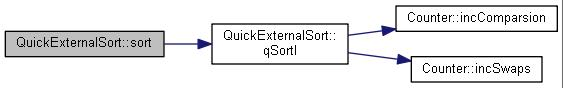
\includegraphics[width=350pt]{class_quick_external_sort_ab277b5945ac22cdcda10bf02e56eb8db_cgraph}
\end{center}
\end{figure}


Объявления и описания членов классов находятся в файлах\+:\begin{DoxyCompactItemize}
\item 
C\+:/\+Users/админ/\+Documents/\+Projects\+C++/\+External\+Merge\+Sort\+Production/\+External\+Merge\+Sort\+Production/\hyperlink{_quick_external_sort_8h}{Quick\+External\+Sort.\+h}\item 
C\+:/\+Users/админ/\+Documents/\+Projects\+C++/\+External\+Merge\+Sort\+Production/\+External\+Merge\+Sort\+Production/\hyperlink{_quick_external_sort_8cpp}{Quick\+External\+Sort.\+cpp}\end{DoxyCompactItemize}

\hypertarget{class_user_interface}{}\section{User\+Interface Class Reference}
\label{class_user_interface}\index{User\+Interface@{User\+Interface}}


Класс пользовательского интерфейса.  




{\ttfamily \#include $<$User\+Interface.\+h$>$}

\subsection*{Public Member Functions}
\begin{DoxyCompactItemize}
\item 
void \hyperlink{class_user_interface_a6c7f9ef9faa40eaf4760d57e89228786}{init\+Session} ()
\item 
\hyperlink{class_user_interface_ae6fb70370701b3bd6120e923df9705b0}{User\+Interface} ()
\item 
\hyperlink{class_user_interface_ae588b2ff1711a016dd4c6fc5002c0841}{$\sim$\+User\+Interface} ()
\end{DoxyCompactItemize}
\subsection*{Private Member Functions}
\begin{DoxyCompactItemize}
\item 
bool \hyperlink{class_user_interface_ad388ff348c0a124038f4ea9756b80041}{call\+Method} (int ch)
\begin{DoxyCompactList}\small\item\em Вызов необходимого метода. \end{DoxyCompactList}\item 
void \hyperlink{class_user_interface_a27c547dadfd5588d5b734e253b2e8a4a}{call\+Generate} ()
\begin{DoxyCompactList}\small\item\em Вызов генерации последовательности. Получает необходимые параметры для генерации исходной последовательности. Оповещает о возникающих ошибках. \end{DoxyCompactList}\item 
void \hyperlink{class_user_interface_adcabf6c8f2be4b4ec712c4674156bf59}{call\+Set\+Params} ()
\begin{DoxyCompactList}\small\item\em Вызов метода, задающего параметры сортировки. Задает параметр sort необходимым указателем на один из классов сортировки. Получает необходимые параметры сортировки. Оповещает о возникающих ошибках. \end{DoxyCompactList}\item 
void \hyperlink{class_user_interface_a0e03dfecee7e890ad1e076888062d5cb}{call\+Sort} ()
\begin{DoxyCompactList}\small\item\em Вызов метода внешней сортировки. Вызывает необходимый метод сортировки, если это возможно. Оповещает о возникающих ошибках. \end{DoxyCompactList}\item 
void \hyperlink{class_user_interface_a7957201b3543ea0561d48bcc0a0d329e}{call\+Estimate} ()
\begin{DoxyCompactList}\small\item\em Вызов метода оценки характеристик внешней сортировки. Вызывает метод сортировки, если это возможно. Оповещает о возникающих ошибках. \end{DoxyCompactList}\item 
void \hyperlink{class_user_interface_a332db63dca89d684f7e9e1272f4c3745}{call\+Get\+Dependencies} ()
\begin{DoxyCompactList}\small\item\em Вызов метода получения зависимостей характеристик сортировки. Вызывает метод сортировки, если это возможно. Оповещает о возникающих ошибках. \end{DoxyCompactList}\item 
\hyperlink{_structures_8h_a9864d6ef28dd6e38416afac4426b3491}{Responce} \hyperlink{class_user_interface_a595a469d83a351719c75c65fbf4a6fbe}{set\+Params} (\hyperlink{class_file_manager}{File\+Manager} $\ast$file, long long size\+Of\+Segments, \hyperlink{_structures_8h_adbb15722785daaf5166f7ea34323854c}{Type\+Of\+Sort} type)
\item 
void \hyperlink{class_user_interface_af7c9d93ec693f70dcfbdd9e6a080abc7}{get\+Dependence\+Size} ()
\item 
void \hyperlink{class_user_interface_aaac8a635efdb79276275f9d1ea265cd7}{get\+Dependence\+Size\+Of\+Segments} ()
\item 
void \hyperlink{class_user_interface_ab726cdce7e7518aae70cf42594139589}{get\+Dependence\+Type} ()
\end{DoxyCompactItemize}
\subsection*{Private Attributes}
\begin{DoxyCompactItemize}
\item 
\hyperlink{class_external_merge_sort}{External\+Merge\+Sort} $\ast$ \hyperlink{class_user_interface_af3405ffdb7e2834c2cf63662b5415a91}{sort}
\begin{DoxyCompactList}\small\item\em Указатель на экземпляр класса сортировки. \end{DoxyCompactList}\item 
const string \hyperlink{class_user_interface_a24b9a8a0a253382b0737a86f7ecf7d8b}{menu} = \char`\"{}0. Выход\textbackslash{}n1. Сгенерировать последовательность\textbackslash{}n2. Задать параметры сортировки\textbackslash{}n3. Отсоритровать последовательность\textbackslash{}n4. Оценить характеристики сортировки\textbackslash{}n5. Получение зависимостей\textbackslash{}n\char`\"{}
\begin{DoxyCompactList}\small\item\em Константная строка меню. \end{DoxyCompactList}\item 
const char $\ast$ \hyperlink{class_user_interface_a3ec4a2871150fd6b83ddf9d459aa0afc}{responce\+String} \mbox{[}9\mbox{]}
\begin{DoxyCompactList}\small\item\em Константный массив, строк, расшифровывающих коды ошибок. \end{DoxyCompactList}\end{DoxyCompactItemize}


\subsection{Detailed Description}
Класс пользовательского интерфейса. 

\begin{DoxyAuthor}{Author}
Alexander Filippov 
\end{DoxyAuthor}
\begin{DoxyDate}{Date}
Ноябрь 2016 года
\end{DoxyDate}
Класс, отвечающий за взаимодействие пользователя с приложением, а также содержащий в себе некоторые методы, которые позволяют исследовать характеристики сортировки. Сообщает об ошибках и выводит результаты в консоль. 

\subsection{Constructor \& Destructor Documentation}
\hypertarget{class_user_interface_ae6fb70370701b3bd6120e923df9705b0}{}\label{class_user_interface_ae6fb70370701b3bd6120e923df9705b0} 
\index{User\+Interface@{User\+Interface}!User\+Interface@{User\+Interface}}
\index{User\+Interface@{User\+Interface}!User\+Interface@{User\+Interface}}
\subsubsection{\texorpdfstring{User\+Interface()}{UserInterface()}}
{\footnotesize\ttfamily User\+Interface\+::\+User\+Interface (\begin{DoxyParamCaption}{ }\end{DoxyParamCaption})}

\hypertarget{class_user_interface_ae588b2ff1711a016dd4c6fc5002c0841}{}\label{class_user_interface_ae588b2ff1711a016dd4c6fc5002c0841} 
\index{User\+Interface@{User\+Interface}!````~User\+Interface@{$\sim$\+User\+Interface}}
\index{````~User\+Interface@{$\sim$\+User\+Interface}!User\+Interface@{User\+Interface}}
\subsubsection{\texorpdfstring{$\sim$\+User\+Interface()}{~UserInterface()}}
{\footnotesize\ttfamily User\+Interface\+::$\sim$\+User\+Interface (\begin{DoxyParamCaption}{ }\end{DoxyParamCaption})}



\subsection{Member Function Documentation}
\hypertarget{class_user_interface_a7957201b3543ea0561d48bcc0a0d329e}{}\label{class_user_interface_a7957201b3543ea0561d48bcc0a0d329e} 
\index{User\+Interface@{User\+Interface}!call\+Estimate@{call\+Estimate}}
\index{call\+Estimate@{call\+Estimate}!User\+Interface@{User\+Interface}}
\subsubsection{\texorpdfstring{call\+Estimate()}{callEstimate()}}
{\footnotesize\ttfamily void User\+Interface\+::call\+Estimate (\begin{DoxyParamCaption}{ }\end{DoxyParamCaption})\hspace{0.3cm}{\ttfamily [private]}}



Вызов метода оценки характеристик внешней сортировки. Вызывает метод сортировки, если это возможно. Оповещает о возникающих ошибках. 

\hypertarget{class_user_interface_a27c547dadfd5588d5b734e253b2e8a4a}{}\label{class_user_interface_a27c547dadfd5588d5b734e253b2e8a4a} 
\index{User\+Interface@{User\+Interface}!call\+Generate@{call\+Generate}}
\index{call\+Generate@{call\+Generate}!User\+Interface@{User\+Interface}}
\subsubsection{\texorpdfstring{call\+Generate()}{callGenerate()}}
{\footnotesize\ttfamily void User\+Interface\+::call\+Generate (\begin{DoxyParamCaption}{ }\end{DoxyParamCaption})\hspace{0.3cm}{\ttfamily [private]}}



Вызов генерации последовательности. Получает необходимые параметры для генерации исходной последовательности. Оповещает о возникающих ошибках. 

\hypertarget{class_user_interface_a332db63dca89d684f7e9e1272f4c3745}{}\label{class_user_interface_a332db63dca89d684f7e9e1272f4c3745} 
\index{User\+Interface@{User\+Interface}!call\+Get\+Dependencies@{call\+Get\+Dependencies}}
\index{call\+Get\+Dependencies@{call\+Get\+Dependencies}!User\+Interface@{User\+Interface}}
\subsubsection{\texorpdfstring{call\+Get\+Dependencies()}{callGetDependencies()}}
{\footnotesize\ttfamily void User\+Interface\+::call\+Get\+Dependencies (\begin{DoxyParamCaption}{ }\end{DoxyParamCaption})\hspace{0.3cm}{\ttfamily [private]}}



Вызов метода получения зависимостей характеристик сортировки. Вызывает метод сортировки, если это возможно. Оповещает о возникающих ошибках. 

\hypertarget{class_user_interface_ad388ff348c0a124038f4ea9756b80041}{}\label{class_user_interface_ad388ff348c0a124038f4ea9756b80041} 
\index{User\+Interface@{User\+Interface}!call\+Method@{call\+Method}}
\index{call\+Method@{call\+Method}!User\+Interface@{User\+Interface}}
\subsubsection{\texorpdfstring{call\+Method()}{callMethod()}}
{\footnotesize\ttfamily bool User\+Interface\+::call\+Method (\begin{DoxyParamCaption}\item[{int}]{ch }\end{DoxyParamCaption})\hspace{0.3cm}{\ttfamily [private]}}



Вызов необходимого метода. 

Вызывает метод, получающий необходимые параметры для выбранной пользователем функциональности. 
\begin{DoxyParams}[1]{Parameters}
\mbox{\tt in}  & {\em ch} & Выбор пользователя \\
\hline
\end{DoxyParams}
\begin{DoxyReturn}{Returns}
Булево значение -\/ если true, то продолжаем работу программу, если нет, то выход из бесконечного цикла. 
\end{DoxyReturn}
\hypertarget{class_user_interface_adcabf6c8f2be4b4ec712c4674156bf59}{}\label{class_user_interface_adcabf6c8f2be4b4ec712c4674156bf59} 
\index{User\+Interface@{User\+Interface}!call\+Set\+Params@{call\+Set\+Params}}
\index{call\+Set\+Params@{call\+Set\+Params}!User\+Interface@{User\+Interface}}
\subsubsection{\texorpdfstring{call\+Set\+Params()}{callSetParams()}}
{\footnotesize\ttfamily void User\+Interface\+::call\+Set\+Params (\begin{DoxyParamCaption}{ }\end{DoxyParamCaption})\hspace{0.3cm}{\ttfamily [private]}}



Вызов метода, задающего параметры сортировки. Задает параметр sort необходимым указателем на один из классов сортировки. Получает необходимые параметры сортировки. Оповещает о возникающих ошибках. 

\hypertarget{class_user_interface_a0e03dfecee7e890ad1e076888062d5cb}{}\label{class_user_interface_a0e03dfecee7e890ad1e076888062d5cb} 
\index{User\+Interface@{User\+Interface}!call\+Sort@{call\+Sort}}
\index{call\+Sort@{call\+Sort}!User\+Interface@{User\+Interface}}
\subsubsection{\texorpdfstring{call\+Sort()}{callSort()}}
{\footnotesize\ttfamily void User\+Interface\+::call\+Sort (\begin{DoxyParamCaption}{ }\end{DoxyParamCaption})\hspace{0.3cm}{\ttfamily [private]}}



Вызов метода внешней сортировки. Вызывает необходимый метод сортировки, если это возможно. Оповещает о возникающих ошибках. 

\hypertarget{class_user_interface_af7c9d93ec693f70dcfbdd9e6a080abc7}{}\label{class_user_interface_af7c9d93ec693f70dcfbdd9e6a080abc7} 
\index{User\+Interface@{User\+Interface}!get\+Dependence\+Size@{get\+Dependence\+Size}}
\index{get\+Dependence\+Size@{get\+Dependence\+Size}!User\+Interface@{User\+Interface}}
\subsubsection{\texorpdfstring{get\+Dependence\+Size()}{getDependenceSize()}}
{\footnotesize\ttfamily void User\+Interface\+::get\+Dependence\+Size (\begin{DoxyParamCaption}{ }\end{DoxyParamCaption})\hspace{0.3cm}{\ttfamily [private]}}

\hypertarget{class_user_interface_aaac8a635efdb79276275f9d1ea265cd7}{}\label{class_user_interface_aaac8a635efdb79276275f9d1ea265cd7} 
\index{User\+Interface@{User\+Interface}!get\+Dependence\+Size\+Of\+Segments@{get\+Dependence\+Size\+Of\+Segments}}
\index{get\+Dependence\+Size\+Of\+Segments@{get\+Dependence\+Size\+Of\+Segments}!User\+Interface@{User\+Interface}}
\subsubsection{\texorpdfstring{get\+Dependence\+Size\+Of\+Segments()}{getDependenceSizeOfSegments()}}
{\footnotesize\ttfamily void User\+Interface\+::get\+Dependence\+Size\+Of\+Segments (\begin{DoxyParamCaption}{ }\end{DoxyParamCaption})\hspace{0.3cm}{\ttfamily [private]}}

\hypertarget{class_user_interface_ab726cdce7e7518aae70cf42594139589}{}\label{class_user_interface_ab726cdce7e7518aae70cf42594139589} 
\index{User\+Interface@{User\+Interface}!get\+Dependence\+Type@{get\+Dependence\+Type}}
\index{get\+Dependence\+Type@{get\+Dependence\+Type}!User\+Interface@{User\+Interface}}
\subsubsection{\texorpdfstring{get\+Dependence\+Type()}{getDependenceType()}}
{\footnotesize\ttfamily void User\+Interface\+::get\+Dependence\+Type (\begin{DoxyParamCaption}{ }\end{DoxyParamCaption})\hspace{0.3cm}{\ttfamily [private]}}

\hypertarget{class_user_interface_a6c7f9ef9faa40eaf4760d57e89228786}{}\label{class_user_interface_a6c7f9ef9faa40eaf4760d57e89228786} 
\index{User\+Interface@{User\+Interface}!init\+Session@{init\+Session}}
\index{init\+Session@{init\+Session}!User\+Interface@{User\+Interface}}
\subsubsection{\texorpdfstring{init\+Session()}{initSession()}}
{\footnotesize\ttfamily void User\+Interface\+::init\+Session (\begin{DoxyParamCaption}{ }\end{DoxyParamCaption})}

\hypertarget{class_user_interface_a595a469d83a351719c75c65fbf4a6fbe}{}\label{class_user_interface_a595a469d83a351719c75c65fbf4a6fbe} 
\index{User\+Interface@{User\+Interface}!set\+Params@{set\+Params}}
\index{set\+Params@{set\+Params}!User\+Interface@{User\+Interface}}
\subsubsection{\texorpdfstring{set\+Params()}{setParams()}}
{\footnotesize\ttfamily \hyperlink{_structures_8h_a9864d6ef28dd6e38416afac4426b3491}{Responce} User\+Interface\+::set\+Params (\begin{DoxyParamCaption}\item[{\hyperlink{class_file_manager}{File\+Manager} $\ast$}]{file,  }\item[{long long}]{size\+Of\+Segments,  }\item[{\hyperlink{_structures_8h_adbb15722785daaf5166f7ea34323854c}{Type\+Of\+Sort}}]{type }\end{DoxyParamCaption})\hspace{0.3cm}{\ttfamily [private]}}



\subsection{Member Data Documentation}
\hypertarget{class_user_interface_a24b9a8a0a253382b0737a86f7ecf7d8b}{}\label{class_user_interface_a24b9a8a0a253382b0737a86f7ecf7d8b} 
\index{User\+Interface@{User\+Interface}!menu@{menu}}
\index{menu@{menu}!User\+Interface@{User\+Interface}}
\subsubsection{\texorpdfstring{menu}{menu}}
{\footnotesize\ttfamily const string User\+Interface\+::menu = \char`\"{}0. Выход\textbackslash{}n1. Сгенерировать последовательность\textbackslash{}n2. Задать параметры сортировки\textbackslash{}n3. Отсоритровать последовательность\textbackslash{}n4. Оценить характеристики сортировки\textbackslash{}n5. Получение зависимостей\textbackslash{}n\char`\"{}\hspace{0.3cm}{\ttfamily [private]}}



Константная строка меню. 

\hypertarget{class_user_interface_a3ec4a2871150fd6b83ddf9d459aa0afc}{}\label{class_user_interface_a3ec4a2871150fd6b83ddf9d459aa0afc} 
\index{User\+Interface@{User\+Interface}!responce\+String@{responce\+String}}
\index{responce\+String@{responce\+String}!User\+Interface@{User\+Interface}}
\subsubsection{\texorpdfstring{responce\+String}{responceString}}
{\footnotesize\ttfamily const char$\ast$ User\+Interface\+::responce\+String\mbox{[}9\mbox{]}\hspace{0.3cm}{\ttfamily [private]}}

{\bfseries Initial value\+:}
\begin{DoxyCode}
= \{ \textcolor{stringliteral}{"Успешно"}, \textcolor{stringliteral}{"Ошибка генерации"}, \textcolor{stringliteral}{"Файл не существует"}, \textcolor{stringliteral}{"Ошибка размера"}, \textcolor{stringliteral}{"Ошибка файл-менеджера"},
        \textcolor{stringliteral}{"Исходный файл и файл результата совпадают"}, \textcolor{stringliteral}{"Достигнут конец файла"}, \textcolor{stringliteral}{"Ошибка выделения памяти"}, \textcolor{stringliteral}{"
      Параметры не заданы или заданы неверно"} \}
\end{DoxyCode}


Константный массив, строк, расшифровывающих коды ошибок. 

\hypertarget{class_user_interface_af3405ffdb7e2834c2cf63662b5415a91}{}\label{class_user_interface_af3405ffdb7e2834c2cf63662b5415a91} 
\index{User\+Interface@{User\+Interface}!sort@{sort}}
\index{sort@{sort}!User\+Interface@{User\+Interface}}
\subsubsection{\texorpdfstring{sort}{sort}}
{\footnotesize\ttfamily \hyperlink{class_external_merge_sort}{External\+Merge\+Sort}$\ast$ User\+Interface\+::sort\hspace{0.3cm}{\ttfamily [private]}}



Указатель на экземпляр класса сортировки. 

Позволяет использовать методы внешней многофазной сортировки слиянием. 

The documentation for this class was generated from the following files\+:\begin{DoxyCompactItemize}
\item 
C\+:/\+Users/админ/\+Documents/\+Projects\+C++/\+External\+Merge\+Sort\+Production/\+External\+Merge\+Sort\+Production/\hyperlink{_user_interface_8h}{User\+Interface.\+h}\item 
C\+:/\+Users/админ/\+Documents/\+Projects\+C++/\+External\+Merge\+Sort\+Production/\+External\+Merge\+Sort\+Production/\hyperlink{_user_interface_8cpp}{User\+Interface.\+cpp}\end{DoxyCompactItemize}

\chapter{File Documentation}
\hypertarget{_bubble_external_sort_8cpp}{}\section{Файл C\+:/\+Users/админ/\+Documents/\+Projects\+C++/\+External\+Merge\+Sort\+Production/\+External\+Merge\+Sort\+Production/\+Bubble\+External\+Sort.cpp}
\label{_bubble_external_sort_8cpp}\index{C\+:/\+Users/админ/\+Documents/\+Projects\+C++/\+External\+Merge\+Sort\+Production/\+External\+Merge\+Sort\+Production/\+Bubble\+External\+Sort.\+cpp@{C\+:/\+Users/админ/\+Documents/\+Projects\+C++/\+External\+Merge\+Sort\+Production/\+External\+Merge\+Sort\+Production/\+Bubble\+External\+Sort.\+cpp}}
{\ttfamily \#include \char`\"{}stdafx.\+h\char`\"{}}\newline
{\ttfamily \#include \char`\"{}Bubble\+External\+Sort.\+h\char`\"{}}\newline
Граф включаемых заголовочных файлов для Bubble\+External\+Sort.\+cpp\+:\nopagebreak
\begin{figure}[H]
\begin{center}
\leavevmode
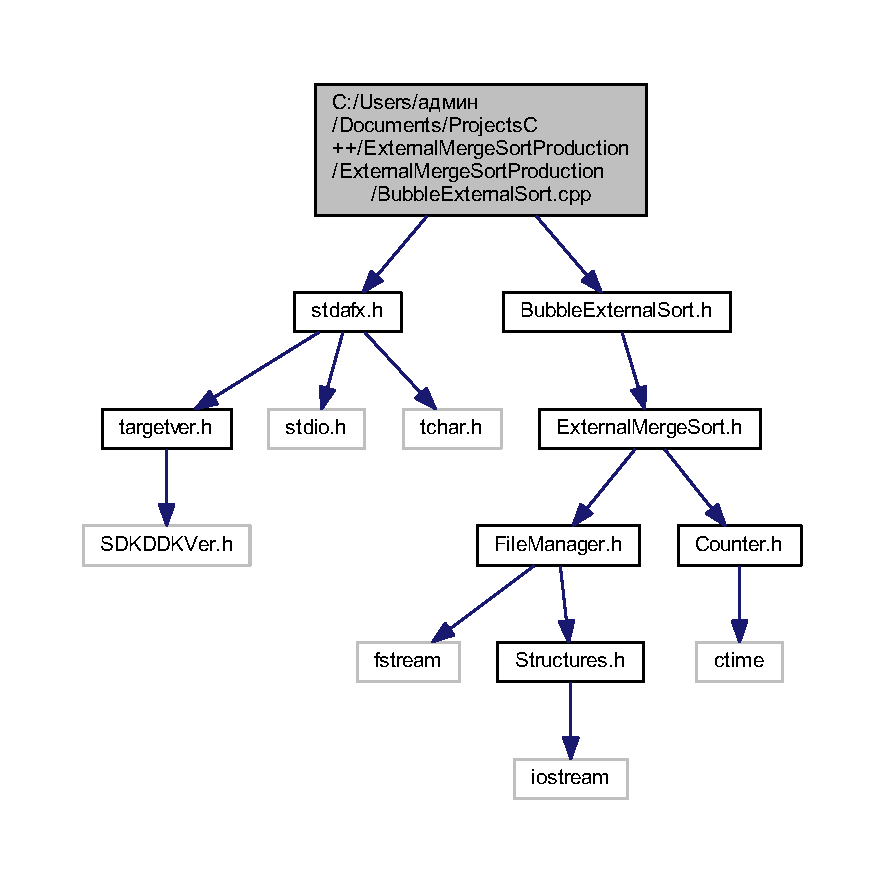
\includegraphics[width=350pt]{_bubble_external_sort_8cpp__incl}
\end{center}
\end{figure}

\hypertarget{_bubble_external_sort_8h}{}\section{Файл C\+:/\+Users/админ/\+Documents/\+Projects\+C++/\+External\+Merge\+Sort\+Production/\+External\+Merge\+Sort\+Production/\+Bubble\+External\+Sort.h}
\label{_bubble_external_sort_8h}\index{C\+:/\+Users/админ/\+Documents/\+Projects\+C++/\+External\+Merge\+Sort\+Production/\+External\+Merge\+Sort\+Production/\+Bubble\+External\+Sort.\+h@{C\+:/\+Users/админ/\+Documents/\+Projects\+C++/\+External\+Merge\+Sort\+Production/\+External\+Merge\+Sort\+Production/\+Bubble\+External\+Sort.\+h}}
{\ttfamily \#include \char`\"{}External\+Merge\+Sort.\+h\char`\"{}}\newline
Граф включаемых заголовочных файлов для Bubble\+External\+Sort.\+h\+:\nopagebreak
\begin{figure}[H]
\begin{center}
\leavevmode
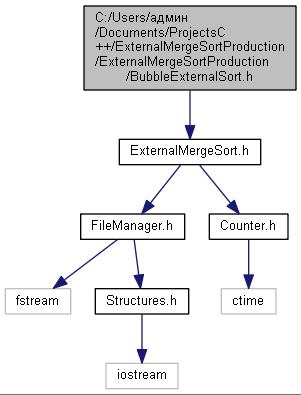
\includegraphics[width=298pt]{_bubble_external_sort_8h__incl}
\end{center}
\end{figure}
Граф файлов, в которые включается этот файл\+:\nopagebreak
\begin{figure}[H]
\begin{center}
\leavevmode
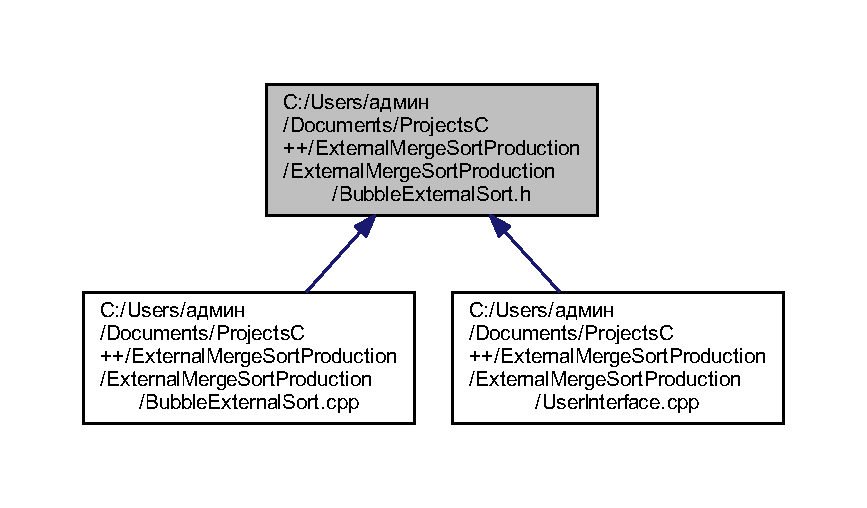
\includegraphics[width=350pt]{_bubble_external_sort_8h__dep__incl}
\end{center}
\end{figure}
\subsection*{Классы}
\begin{DoxyCompactItemize}
\item 
class \hyperlink{class_bubble_external_sort}{Bubble\+External\+Sort}
\end{DoxyCompactItemize}

\hypertarget{_counter_8cpp}{}\section{Файл C\+:/\+Users/админ/\+Documents/\+Projects\+C++/\+External\+Merge\+Sort\+Production/\+External\+Merge\+Sort\+Production/\+Counter.cpp}
\label{_counter_8cpp}\index{C\+:/\+Users/админ/\+Documents/\+Projects\+C++/\+External\+Merge\+Sort\+Production/\+External\+Merge\+Sort\+Production/\+Counter.\+cpp@{C\+:/\+Users/админ/\+Documents/\+Projects\+C++/\+External\+Merge\+Sort\+Production/\+External\+Merge\+Sort\+Production/\+Counter.\+cpp}}
{\ttfamily \#include \char`\"{}stdafx.\+h\char`\"{}}\newline
{\ttfamily \#include \char`\"{}Counter.\+h\char`\"{}}\newline
Граф включаемых заголовочных файлов для Counter.\+cpp\+:\nopagebreak
\begin{figure}[H]
\begin{center}
\leavevmode
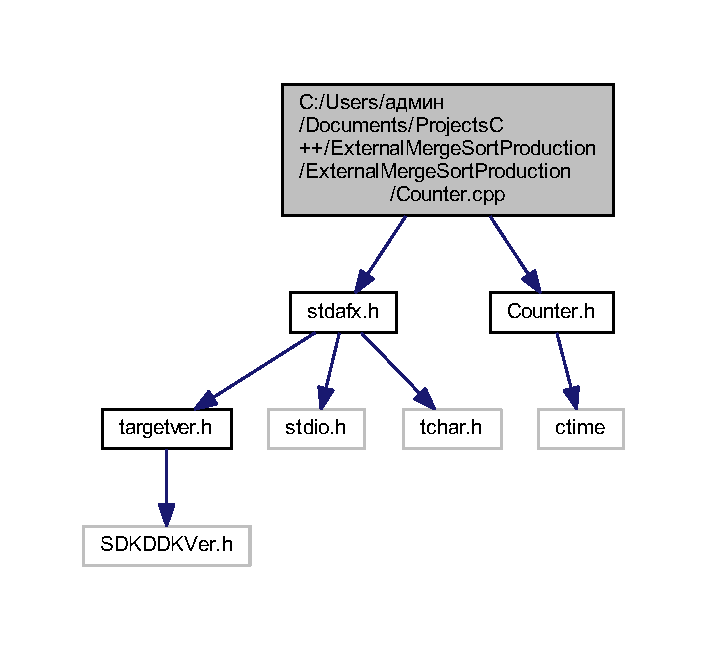
\includegraphics[width=340pt]{_counter_8cpp__incl}
\end{center}
\end{figure}

\hypertarget{_counter_8h}{}\section{Файл C\+:/\+Users/админ/\+Documents/\+Projects\+C++/\+External\+Merge\+Sort\+Production/\+External\+Merge\+Sort\+Production/\+Counter.h}
\label{_counter_8h}\index{C\+:/\+Users/админ/\+Documents/\+Projects\+C++/\+External\+Merge\+Sort\+Production/\+External\+Merge\+Sort\+Production/\+Counter.\+h@{C\+:/\+Users/админ/\+Documents/\+Projects\+C++/\+External\+Merge\+Sort\+Production/\+External\+Merge\+Sort\+Production/\+Counter.\+h}}
{\ttfamily \#include $<$ctime$>$}\newline
Граф включаемых заголовочных файлов для Counter.\+h\+:\nopagebreak
\begin{figure}[H]
\begin{center}
\leavevmode
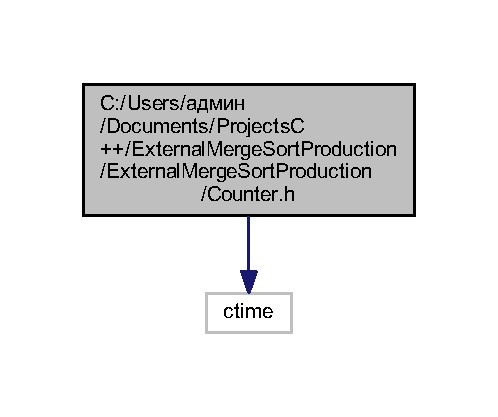
\includegraphics[width=239pt]{_counter_8h__incl}
\end{center}
\end{figure}
Граф файлов, в которые включается этот файл\+:\nopagebreak
\begin{figure}[H]
\begin{center}
\leavevmode
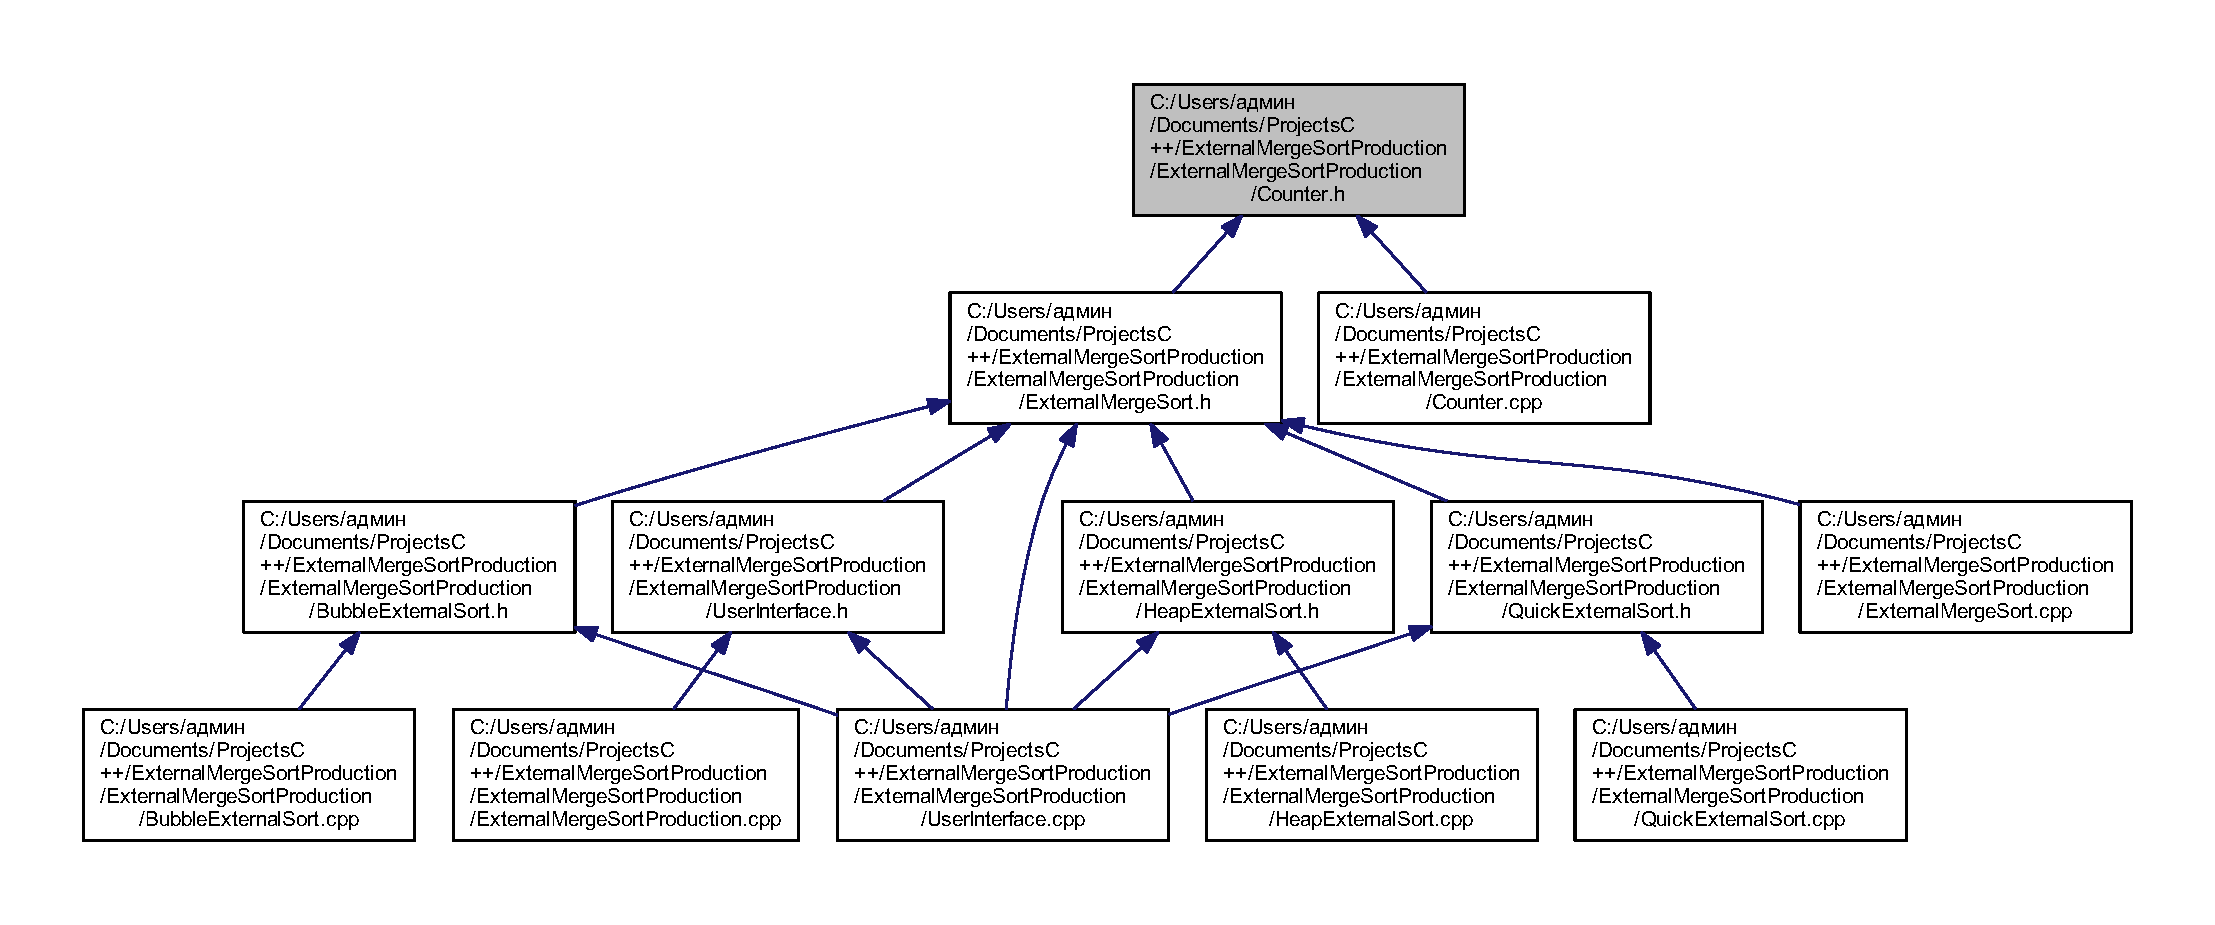
\includegraphics[width=350pt]{_counter_8h__dep__incl}
\end{center}
\end{figure}
\subsection*{Классы}
\begin{DoxyCompactItemize}
\item 
class \hyperlink{class_counter}{Counter}
\end{DoxyCompactItemize}

\hypertarget{_external_merge_sort_8cpp}{}\section{Файл C\+:/\+Users/админ/\+Documents/\+Projects\+C++/\+External\+Merge\+Sort\+Production/\+External\+Merge\+Sort\+Production/\+External\+Merge\+Sort.cpp}
\label{_external_merge_sort_8cpp}\index{C\+:/\+Users/админ/\+Documents/\+Projects\+C++/\+External\+Merge\+Sort\+Production/\+External\+Merge\+Sort\+Production/\+External\+Merge\+Sort.\+cpp@{C\+:/\+Users/админ/\+Documents/\+Projects\+C++/\+External\+Merge\+Sort\+Production/\+External\+Merge\+Sort\+Production/\+External\+Merge\+Sort.\+cpp}}
{\ttfamily \#include \char`\"{}stdafx.\+h\char`\"{}}\newline
{\ttfamily \#include \char`\"{}External\+Merge\+Sort.\+h\char`\"{}}\newline
{\ttfamily \#include $<$sstream$>$}\newline
Граф включаемых заголовочных файлов для External\+Merge\+Sort.\+cpp\+:\nopagebreak
\begin{figure}[H]
\begin{center}
\leavevmode
\includegraphics[width=350pt]{_external_merge_sort_8cpp__incl}
\end{center}
\end{figure}

\hypertarget{_external_merge_sort_8h}{}\section{Файл C\+:/\+Users/админ/\+Documents/\+Projects\+C++/\+External\+Merge\+Sort\+Production/\+External\+Merge\+Sort\+Production/\+External\+Merge\+Sort.h}
\label{_external_merge_sort_8h}\index{C\+:/\+Users/админ/\+Documents/\+Projects\+C++/\+External\+Merge\+Sort\+Production/\+External\+Merge\+Sort\+Production/\+External\+Merge\+Sort.\+h@{C\+:/\+Users/админ/\+Documents/\+Projects\+C++/\+External\+Merge\+Sort\+Production/\+External\+Merge\+Sort\+Production/\+External\+Merge\+Sort.\+h}}
{\ttfamily \#include \char`\"{}File\+Manager.\+h\char`\"{}}\newline
{\ttfamily \#include \char`\"{}Counter.\+h\char`\"{}}\newline
Граф включаемых заголовочных файлов для External\+Merge\+Sort.\+h\+:\nopagebreak
\begin{figure}[H]
\begin{center}
\leavevmode
\includegraphics[width=298pt]{_external_merge_sort_8h__incl}
\end{center}
\end{figure}
Граф файлов, в которые включается этот файл\+:\nopagebreak
\begin{figure}[H]
\begin{center}
\leavevmode
\includegraphics[width=350pt]{_external_merge_sort_8h__dep__incl}
\end{center}
\end{figure}
\subsection*{Классы}
\begin{DoxyCompactItemize}
\item 
class \hyperlink{class_external_merge_sort}{External\+Merge\+Sort}
\end{DoxyCompactItemize}

\hypertarget{_external_merge_sort_production_8cpp}{}\section{Файл C\+:/\+Users/админ/\+Documents/\+Projects\+C++/\+External\+Merge\+Sort\+Production/\+External\+Merge\+Sort\+Production/\+External\+Merge\+Sort\+Production.cpp}
\label{_external_merge_sort_production_8cpp}\index{C\+:/\+Users/админ/\+Documents/\+Projects\+C++/\+External\+Merge\+Sort\+Production/\+External\+Merge\+Sort\+Production/\+External\+Merge\+Sort\+Production.\+cpp@{C\+:/\+Users/админ/\+Documents/\+Projects\+C++/\+External\+Merge\+Sort\+Production/\+External\+Merge\+Sort\+Production/\+External\+Merge\+Sort\+Production.\+cpp}}
{\ttfamily \#include \char`\"{}stdafx.\+h\char`\"{}}\newline
{\ttfamily \#include \char`\"{}User\+Interface.\+h\char`\"{}}\newline
{\ttfamily \#include $<$iostream$>$}\newline
Граф включаемых заголовочных файлов для External\+Merge\+Sort\+Production.\+cpp\+:\nopagebreak
\begin{figure}[H]
\begin{center}
\leavevmode
\includegraphics[width=350pt]{_external_merge_sort_production_8cpp__incl}
\end{center}
\end{figure}
\subsection*{Функции}
\begin{DoxyCompactItemize}
\item 
int \hyperlink{_external_merge_sort_production_8cpp_ae66f6b31b5ad750f1fe042a706a4e3d4}{main} ()
\end{DoxyCompactItemize}


\subsection{Функции}
\hypertarget{_external_merge_sort_production_8cpp_ae66f6b31b5ad750f1fe042a706a4e3d4}{}\label{_external_merge_sort_production_8cpp_ae66f6b31b5ad750f1fe042a706a4e3d4} 
\index{External\+Merge\+Sort\+Production.\+cpp@{External\+Merge\+Sort\+Production.\+cpp}!main@{main}}
\index{main@{main}!External\+Merge\+Sort\+Production.\+cpp@{External\+Merge\+Sort\+Production.\+cpp}}
\subsubsection{\texorpdfstring{main()}{main()}}
{\footnotesize\ttfamily int main (\begin{DoxyParamCaption}{ }\end{DoxyParamCaption})}

Граф вызовов\+:\nopagebreak
\begin{figure}[H]
\begin{center}
\leavevmode
\includegraphics[width=282pt]{_external_merge_sort_production_8cpp_ae66f6b31b5ad750f1fe042a706a4e3d4_cgraph}
\end{center}
\end{figure}

\hypertarget{_file_manager_8cpp}{}\section{Файл C\+:/\+Users/админ/\+Documents/\+Projects\+C++/\+External\+Merge\+Sort\+Production/\+External\+Merge\+Sort\+Production/\+File\+Manager.cpp}
\label{_file_manager_8cpp}\index{C\+:/\+Users/админ/\+Documents/\+Projects\+C++/\+External\+Merge\+Sort\+Production/\+External\+Merge\+Sort\+Production/\+File\+Manager.\+cpp@{C\+:/\+Users/админ/\+Documents/\+Projects\+C++/\+External\+Merge\+Sort\+Production/\+External\+Merge\+Sort\+Production/\+File\+Manager.\+cpp}}
{\ttfamily \#include \char`\"{}stdafx.\+h\char`\"{}}\newline
{\ttfamily \#include \char`\"{}File\+Manager.\+h\char`\"{}}\newline
{\ttfamily \#include $<$random$>$}\newline
{\ttfamily \#include $<$ctime$>$}\newline
{\ttfamily \#include $<$iostream$>$}\newline
{\ttfamily \#include $<$sstream$>$}\newline
Граф включаемых заголовочных файлов для File\+Manager.\+cpp\+:\nopagebreak
\begin{figure}[H]
\begin{center}
\leavevmode
\includegraphics[width=350pt]{_file_manager_8cpp__incl}
\end{center}
\end{figure}

\hypertarget{_file_manager_8h}{}\section{Файл C\+:/\+Users/админ/\+Documents/\+Projects\+C++/\+External\+Merge\+Sort\+Production/\+External\+Merge\+Sort\+Production/\+File\+Manager.h}
\label{_file_manager_8h}\index{C\+:/\+Users/админ/\+Documents/\+Projects\+C++/\+External\+Merge\+Sort\+Production/\+External\+Merge\+Sort\+Production/\+File\+Manager.\+h@{C\+:/\+Users/админ/\+Documents/\+Projects\+C++/\+External\+Merge\+Sort\+Production/\+External\+Merge\+Sort\+Production/\+File\+Manager.\+h}}
{\ttfamily \#include $<$fstream$>$}\newline
{\ttfamily \#include \char`\"{}Structures.\+h\char`\"{}}\newline
Граф включаемых заголовочных файлов для File\+Manager.\+h\+:\nopagebreak
\begin{figure}[H]
\begin{center}
\leavevmode
\includegraphics[width=239pt]{_file_manager_8h__incl}
\end{center}
\end{figure}
Граф файлов, в которые включается этот файл\+:\nopagebreak
\begin{figure}[H]
\begin{center}
\leavevmode
\includegraphics[width=350pt]{_file_manager_8h__dep__incl}
\end{center}
\end{figure}
\subsection*{Классы}
\begin{DoxyCompactItemize}
\item 
class \hyperlink{class_file_manager}{File\+Manager}
\begin{DoxyCompactList}\small\item\em Класс файлового менеджера. \end{DoxyCompactList}\end{DoxyCompactItemize}

\hypertarget{_heap_external_sort_8cpp}{}\section{Файл C\+:/\+Users/админ/\+Documents/\+Projects\+C++/\+External\+Merge\+Sort\+Production/\+External\+Merge\+Sort\+Production/\+Heap\+External\+Sort.cpp}
\label{_heap_external_sort_8cpp}\index{C\+:/\+Users/админ/\+Documents/\+Projects\+C++/\+External\+Merge\+Sort\+Production/\+External\+Merge\+Sort\+Production/\+Heap\+External\+Sort.\+cpp@{C\+:/\+Users/админ/\+Documents/\+Projects\+C++/\+External\+Merge\+Sort\+Production/\+External\+Merge\+Sort\+Production/\+Heap\+External\+Sort.\+cpp}}
{\ttfamily \#include \char`\"{}stdafx.\+h\char`\"{}}\newline
{\ttfamily \#include \char`\"{}Heap\+External\+Sort.\+h\char`\"{}}\newline
Граф включаемых заголовочных файлов для Heap\+External\+Sort.\+cpp\+:\nopagebreak
\begin{figure}[H]
\begin{center}
\leavevmode
\includegraphics[width=350pt]{_heap_external_sort_8cpp__incl}
\end{center}
\end{figure}

\hypertarget{_heap_external_sort_8h}{}\section{Файл C\+:/\+Users/админ/\+Documents/\+Projects\+C++/\+External\+Merge\+Sort\+Production/\+External\+Merge\+Sort\+Production/\+Heap\+External\+Sort.h}
\label{_heap_external_sort_8h}\index{C\+:/\+Users/админ/\+Documents/\+Projects\+C++/\+External\+Merge\+Sort\+Production/\+External\+Merge\+Sort\+Production/\+Heap\+External\+Sort.\+h@{C\+:/\+Users/админ/\+Documents/\+Projects\+C++/\+External\+Merge\+Sort\+Production/\+External\+Merge\+Sort\+Production/\+Heap\+External\+Sort.\+h}}
{\ttfamily \#include \char`\"{}External\+Merge\+Sort.\+h\char`\"{}}\newline
Граф включаемых заголовочных файлов для Heap\+External\+Sort.\+h\+:\nopagebreak
\begin{figure}[H]
\begin{center}
\leavevmode
\includegraphics[width=298pt]{_heap_external_sort_8h__incl}
\end{center}
\end{figure}
Граф файлов, в которые включается этот файл\+:\nopagebreak
\begin{figure}[H]
\begin{center}
\leavevmode
\includegraphics[width=350pt]{_heap_external_sort_8h__dep__incl}
\end{center}
\end{figure}
\subsection*{Классы}
\begin{DoxyCompactItemize}
\item 
class \hyperlink{class_heap_external_sort}{Heap\+External\+Sort}
\end{DoxyCompactItemize}

\hypertarget{_quick_external_sort_8cpp}{}\section{Файл C\+:/\+Users/админ/\+Documents/\+Projects\+C++/\+External\+Merge\+Sort\+Production/\+External\+Merge\+Sort\+Production/\+Quick\+External\+Sort.cpp}
\label{_quick_external_sort_8cpp}\index{C\+:/\+Users/админ/\+Documents/\+Projects\+C++/\+External\+Merge\+Sort\+Production/\+External\+Merge\+Sort\+Production/\+Quick\+External\+Sort.\+cpp@{C\+:/\+Users/админ/\+Documents/\+Projects\+C++/\+External\+Merge\+Sort\+Production/\+External\+Merge\+Sort\+Production/\+Quick\+External\+Sort.\+cpp}}
{\ttfamily \#include \char`\"{}stdafx.\+h\char`\"{}}\newline
{\ttfamily \#include \char`\"{}Quick\+External\+Sort.\+h\char`\"{}}\newline
Граф включаемых заголовочных файлов для Quick\+External\+Sort.\+cpp\+:\nopagebreak
\begin{figure}[H]
\begin{center}
\leavevmode
\includegraphics[width=350pt]{_quick_external_sort_8cpp__incl}
\end{center}
\end{figure}
\subsection*{Макросы}
\begin{DoxyCompactItemize}
\item 
\#define \hyperlink{_quick_external_sort_8cpp_aacca6649d32984be8e1aa076bf42fe46}{M\+A\+X\+S\+T\+A\+CK}~10000
\end{DoxyCompactItemize}


\subsection{Макросы}
\hypertarget{_quick_external_sort_8cpp_aacca6649d32984be8e1aa076bf42fe46}{}\label{_quick_external_sort_8cpp_aacca6649d32984be8e1aa076bf42fe46} 
\index{Quick\+External\+Sort.\+cpp@{Quick\+External\+Sort.\+cpp}!M\+A\+X\+S\+T\+A\+CK@{M\+A\+X\+S\+T\+A\+CK}}
\index{M\+A\+X\+S\+T\+A\+CK@{M\+A\+X\+S\+T\+A\+CK}!Quick\+External\+Sort.\+cpp@{Quick\+External\+Sort.\+cpp}}
\subsubsection{\texorpdfstring{M\+A\+X\+S\+T\+A\+CK}{MAXSTACK}}
{\footnotesize\ttfamily \#define M\+A\+X\+S\+T\+A\+CK~10000}


\hypertarget{_quick_external_sort_8h}{}\section{C\+:/\+Users/админ/\+Documents/\+Projects\+C++/\+External\+Merge\+Sort\+Production/\+External\+Merge\+Sort\+Production/\+Quick\+External\+Sort.h File Reference}
\label{_quick_external_sort_8h}\index{C\+:/\+Users/админ/\+Documents/\+Projects\+C++/\+External\+Merge\+Sort\+Production/\+External\+Merge\+Sort\+Production/\+Quick\+External\+Sort.\+h@{C\+:/\+Users/админ/\+Documents/\+Projects\+C++/\+External\+Merge\+Sort\+Production/\+External\+Merge\+Sort\+Production/\+Quick\+External\+Sort.\+h}}
{\ttfamily \#include \char`\"{}External\+Merge\+Sort.\+h\char`\"{}}\newline
\subsection*{Classes}
\begin{DoxyCompactItemize}
\item 
class \hyperlink{class_quick_external_sort}{Quick\+External\+Sort}
\end{DoxyCompactItemize}

\hypertarget{stdafx_8cpp}{}\section{C\+:/\+Users/админ/\+Documents/\+Projects\+C++/\+External\+Merge\+Sort\+Production/\+External\+Merge\+Sort\+Production/stdafx.cpp File Reference}
\label{stdafx_8cpp}\index{C\+:/\+Users/админ/\+Documents/\+Projects\+C++/\+External\+Merge\+Sort\+Production/\+External\+Merge\+Sort\+Production/stdafx.\+cpp@{C\+:/\+Users/админ/\+Documents/\+Projects\+C++/\+External\+Merge\+Sort\+Production/\+External\+Merge\+Sort\+Production/stdafx.\+cpp}}
{\ttfamily \#include \char`\"{}stdafx.\+h\char`\"{}}\newline
{\ttfamily \#include $<$iostream$>$}\newline

\hypertarget{stdafx_8h}{}\section{Файл C\+:/\+Users/админ/\+Documents/\+Projects\+C++/\+External\+Merge\+Sort\+Production/\+External\+Merge\+Sort\+Production/stdafx.h}
\label{stdafx_8h}\index{C\+:/\+Users/админ/\+Documents/\+Projects\+C++/\+External\+Merge\+Sort\+Production/\+External\+Merge\+Sort\+Production/stdafx.\+h@{C\+:/\+Users/админ/\+Documents/\+Projects\+C++/\+External\+Merge\+Sort\+Production/\+External\+Merge\+Sort\+Production/stdafx.\+h}}
{\ttfamily \#include \char`\"{}targetver.\+h\char`\"{}}\newline
{\ttfamily \#include $<$stdio.\+h$>$}\newline
{\ttfamily \#include $<$tchar.\+h$>$}\newline
Граф включаемых заголовочных файлов для stdafx.\+h\+:\nopagebreak
\begin{figure}[H]
\begin{center}
\leavevmode
\includegraphics[width=281pt]{stdafx_8h__incl}
\end{center}
\end{figure}
Граф файлов, в которые включается этот файл\+:\nopagebreak
\begin{figure}[H]
\begin{center}
\leavevmode
\includegraphics[width=350pt]{stdafx_8h__dep__incl}
\end{center}
\end{figure}

\hypertarget{_structures_8h}{}\section{C\+:/\+Users/админ/\+Documents/\+Projects\+C++/\+External\+Merge\+Sort\+Production/\+External\+Merge\+Sort\+Production/\+Structures.h File Reference}
\label{_structures_8h}\index{C\+:/\+Users/админ/\+Documents/\+Projects\+C++/\+External\+Merge\+Sort\+Production/\+External\+Merge\+Sort\+Production/\+Structures.\+h@{C\+:/\+Users/админ/\+Documents/\+Projects\+C++/\+External\+Merge\+Sort\+Production/\+External\+Merge\+Sort\+Production/\+Structures.\+h}}
{\ttfamily \#include $<$iostream$>$}\newline
\subsection*{Enumerations}
\begin{DoxyCompactItemize}
\item 
enum \hyperlink{_structures_8h_a57306ae0f9e356347388234ed69e0ce7}{File\+State} \{ \hyperlink{_structures_8h_a57306ae0f9e356347388234ed69e0ce7a9a09d6d440bf6910da205465d7b2e4a0}{Not\+Enable}, 
\hyperlink{_structures_8h_a57306ae0f9e356347388234ed69e0ce7af1a03d8a79e3c6ef4a82a0ba3fec6e7a}{Read\+Only}, 
\hyperlink{_structures_8h_a57306ae0f9e356347388234ed69e0ce7a068f8c22e7e359d9000e7d3a4a809b4c}{Write\+Only}, 
\hyperlink{_structures_8h_a57306ae0f9e356347388234ed69e0ce7adbd4a235a28913887d590855a0182027}{Read\+And\+Write}
 \}
\item 
enum \hyperlink{_structures_8h_a9864d6ef28dd6e38416afac4426b3491}{Responce} \{ \newline
\hyperlink{_structures_8h_a9864d6ef28dd6e38416afac4426b3491afdfbdf3247bd36a1f17270d5cec74c9c}{Success}, 
\hyperlink{_structures_8h_a9864d6ef28dd6e38416afac4426b3491aeec752b095431b8fca92ea1de18c3d4b}{Generate\+Error}, 
\hyperlink{_structures_8h_a9864d6ef28dd6e38416afac4426b3491a49a6cae1823ee32326b168d49f2735b7}{File\+Not\+Exist}, 
\hyperlink{_structures_8h_a9864d6ef28dd6e38416afac4426b3491aff5e0c4e167b2a74a058ba96eb0ee149}{Size\+Error}, 
\newline
\hyperlink{_structures_8h_a9864d6ef28dd6e38416afac4426b3491aa5b6b995bdadf7226b96bb9dfd33a3cd}{File\+Manager\+Fail}, 
\hyperlink{_structures_8h_a9864d6ef28dd6e38416afac4426b3491aebd38049a88fe839c522d0352fedda6c}{Input\+And\+Output\+Is\+Equal}, 
\hyperlink{_structures_8h_a9864d6ef28dd6e38416afac4426b3491a54bad0135864f0edc76a7d2ac5e8c0eb}{End\+Of\+File}, 
\hyperlink{_structures_8h_a9864d6ef28dd6e38416afac4426b3491ae78c711dd9a3a19d8175eb124b17611c}{Memory\+Error}, 
\newline
\hyperlink{_structures_8h_a9864d6ef28dd6e38416afac4426b3491ab62878ccac0c970717a5464bb0984be4}{Params\+Fail}
 \}
\item 
enum \hyperlink{_structures_8h_af67907baa897e9fb84df0cb89795b87c}{Log\+Type} \{ \hyperlink{_structures_8h_af67907baa897e9fb84df0cb89795b87cad0125052d862ba0d1091df092c091bf0}{With\+Out}, 
\hyperlink{_structures_8h_af67907baa897e9fb84df0cb89795b87ca172e8dc95b033321bf58a216636307c9}{C\+LI}, 
\hyperlink{_structures_8h_af67907baa897e9fb84df0cb89795b87ca1ab5ebbd194ab0b95e5697aca9ba274f}{File}
 \}
\item 
enum \hyperlink{_structures_8h_a76639e910448c3333d0f4d204e53c2c1}{Seq\+Type} \{ \hyperlink{_structures_8h_a76639e910448c3333d0f4d204e53c2c1a29d9ba0e499ea8fcd3d7b4e3fdc89b75}{Best}, 
\hyperlink{_structures_8h_a76639e910448c3333d0f4d204e53c2c1ab3c87ec2c47256239220b24e46acda7f}{Average}, 
\hyperlink{_structures_8h_a76639e910448c3333d0f4d204e53c2c1a9c59fe574f32e751672580cebf9764ae}{Worst}
 \}
\item 
enum \hyperlink{_structures_8h_adbb15722785daaf5166f7ea34323854c}{Type\+Of\+Sort} \{ \hyperlink{_structures_8h_adbb15722785daaf5166f7ea34323854ca2bd4f97892c8b7d060e9f67527f0b9ef}{Bubble}, 
\hyperlink{_structures_8h_adbb15722785daaf5166f7ea34323854cab6dc6b578a22d35f3d364f3c4ba34c02}{Quick}, 
\hyperlink{_structures_8h_adbb15722785daaf5166f7ea34323854ca139b64ba62923e002df5e9124e778c64}{Heap}, 
\hyperlink{_structures_8h_adbb15722785daaf5166f7ea34323854ca2c88d6b09611bebcfd079df624ae3bfe}{Fail}
 \}
\end{DoxyCompactItemize}


\subsection{Enumeration Type Documentation}
\hypertarget{_structures_8h_a57306ae0f9e356347388234ed69e0ce7}{}\label{_structures_8h_a57306ae0f9e356347388234ed69e0ce7} 
\index{Structures.\+h@{Structures.\+h}!File\+State@{File\+State}}
\index{File\+State@{File\+State}!Structures.\+h@{Structures.\+h}}
\subsubsection{\texorpdfstring{File\+State}{FileState}}
{\footnotesize\ttfamily enum \hyperlink{_structures_8h_a57306ae0f9e356347388234ed69e0ce7}{File\+State}}

\begin{DoxyEnumFields}{Enumerator}
\raisebox{\heightof{T}}[0pt][0pt]{\index{Not\+Enable@{Not\+Enable}!Structures.\+h@{Structures.\+h}}\index{Structures.\+h@{Structures.\+h}!Not\+Enable@{Not\+Enable}}}\hypertarget{_structures_8h_a57306ae0f9e356347388234ed69e0ce7a9a09d6d440bf6910da205465d7b2e4a0}{}\label{_structures_8h_a57306ae0f9e356347388234ed69e0ce7a9a09d6d440bf6910da205465d7b2e4a0} 
Not\+Enable&\\
\hline

\raisebox{\heightof{T}}[0pt][0pt]{\index{Read\+Only@{Read\+Only}!Structures.\+h@{Structures.\+h}}\index{Structures.\+h@{Structures.\+h}!Read\+Only@{Read\+Only}}}\hypertarget{_structures_8h_a57306ae0f9e356347388234ed69e0ce7af1a03d8a79e3c6ef4a82a0ba3fec6e7a}{}\label{_structures_8h_a57306ae0f9e356347388234ed69e0ce7af1a03d8a79e3c6ef4a82a0ba3fec6e7a} 
Read\+Only&\\
\hline

\raisebox{\heightof{T}}[0pt][0pt]{\index{Write\+Only@{Write\+Only}!Structures.\+h@{Structures.\+h}}\index{Structures.\+h@{Structures.\+h}!Write\+Only@{Write\+Only}}}\hypertarget{_structures_8h_a57306ae0f9e356347388234ed69e0ce7a068f8c22e7e359d9000e7d3a4a809b4c}{}\label{_structures_8h_a57306ae0f9e356347388234ed69e0ce7a068f8c22e7e359d9000e7d3a4a809b4c} 
Write\+Only&\\
\hline

\raisebox{\heightof{T}}[0pt][0pt]{\index{Read\+And\+Write@{Read\+And\+Write}!Structures.\+h@{Structures.\+h}}\index{Structures.\+h@{Structures.\+h}!Read\+And\+Write@{Read\+And\+Write}}}\hypertarget{_structures_8h_a57306ae0f9e356347388234ed69e0ce7adbd4a235a28913887d590855a0182027}{}\label{_structures_8h_a57306ae0f9e356347388234ed69e0ce7adbd4a235a28913887d590855a0182027} 
Read\+And\+Write&\\
\hline

\end{DoxyEnumFields}
\hypertarget{_structures_8h_af67907baa897e9fb84df0cb89795b87c}{}\label{_structures_8h_af67907baa897e9fb84df0cb89795b87c} 
\index{Structures.\+h@{Structures.\+h}!Log\+Type@{Log\+Type}}
\index{Log\+Type@{Log\+Type}!Structures.\+h@{Structures.\+h}}
\subsubsection{\texorpdfstring{Log\+Type}{LogType}}
{\footnotesize\ttfamily enum \hyperlink{_structures_8h_af67907baa897e9fb84df0cb89795b87c}{Log\+Type}}

\begin{DoxyEnumFields}{Enumerator}
\raisebox{\heightof{T}}[0pt][0pt]{\index{With\+Out@{With\+Out}!Structures.\+h@{Structures.\+h}}\index{Structures.\+h@{Structures.\+h}!With\+Out@{With\+Out}}}\hypertarget{_structures_8h_af67907baa897e9fb84df0cb89795b87cad0125052d862ba0d1091df092c091bf0}{}\label{_structures_8h_af67907baa897e9fb84df0cb89795b87cad0125052d862ba0d1091df092c091bf0} 
With\+Out&\\
\hline

\raisebox{\heightof{T}}[0pt][0pt]{\index{C\+LI@{C\+LI}!Structures.\+h@{Structures.\+h}}\index{Structures.\+h@{Structures.\+h}!C\+LI@{C\+LI}}}\hypertarget{_structures_8h_af67907baa897e9fb84df0cb89795b87ca172e8dc95b033321bf58a216636307c9}{}\label{_structures_8h_af67907baa897e9fb84df0cb89795b87ca172e8dc95b033321bf58a216636307c9} 
C\+LI&\\
\hline

\raisebox{\heightof{T}}[0pt][0pt]{\index{File@{File}!Structures.\+h@{Structures.\+h}}\index{Structures.\+h@{Structures.\+h}!File@{File}}}\hypertarget{_structures_8h_af67907baa897e9fb84df0cb89795b87ca1ab5ebbd194ab0b95e5697aca9ba274f}{}\label{_structures_8h_af67907baa897e9fb84df0cb89795b87ca1ab5ebbd194ab0b95e5697aca9ba274f} 
File&\\
\hline

\end{DoxyEnumFields}
\hypertarget{_structures_8h_a9864d6ef28dd6e38416afac4426b3491}{}\label{_structures_8h_a9864d6ef28dd6e38416afac4426b3491} 
\index{Structures.\+h@{Structures.\+h}!Responce@{Responce}}
\index{Responce@{Responce}!Structures.\+h@{Structures.\+h}}
\subsubsection{\texorpdfstring{Responce}{Responce}}
{\footnotesize\ttfamily enum \hyperlink{_structures_8h_a9864d6ef28dd6e38416afac4426b3491}{Responce}}

\begin{DoxyEnumFields}{Enumerator}
\raisebox{\heightof{T}}[0pt][0pt]{\index{Success@{Success}!Structures.\+h@{Structures.\+h}}\index{Structures.\+h@{Structures.\+h}!Success@{Success}}}\hypertarget{_structures_8h_a9864d6ef28dd6e38416afac4426b3491afdfbdf3247bd36a1f17270d5cec74c9c}{}\label{_structures_8h_a9864d6ef28dd6e38416afac4426b3491afdfbdf3247bd36a1f17270d5cec74c9c} 
Success&\\
\hline

\raisebox{\heightof{T}}[0pt][0pt]{\index{Generate\+Error@{Generate\+Error}!Structures.\+h@{Structures.\+h}}\index{Structures.\+h@{Structures.\+h}!Generate\+Error@{Generate\+Error}}}\hypertarget{_structures_8h_a9864d6ef28dd6e38416afac4426b3491aeec752b095431b8fca92ea1de18c3d4b}{}\label{_structures_8h_a9864d6ef28dd6e38416afac4426b3491aeec752b095431b8fca92ea1de18c3d4b} 
Generate\+Error&\\
\hline

\raisebox{\heightof{T}}[0pt][0pt]{\index{File\+Not\+Exist@{File\+Not\+Exist}!Structures.\+h@{Structures.\+h}}\index{Structures.\+h@{Structures.\+h}!File\+Not\+Exist@{File\+Not\+Exist}}}\hypertarget{_structures_8h_a9864d6ef28dd6e38416afac4426b3491a49a6cae1823ee32326b168d49f2735b7}{}\label{_structures_8h_a9864d6ef28dd6e38416afac4426b3491a49a6cae1823ee32326b168d49f2735b7} 
File\+Not\+Exist&\\
\hline

\raisebox{\heightof{T}}[0pt][0pt]{\index{Size\+Error@{Size\+Error}!Structures.\+h@{Structures.\+h}}\index{Structures.\+h@{Structures.\+h}!Size\+Error@{Size\+Error}}}\hypertarget{_structures_8h_a9864d6ef28dd6e38416afac4426b3491aff5e0c4e167b2a74a058ba96eb0ee149}{}\label{_structures_8h_a9864d6ef28dd6e38416afac4426b3491aff5e0c4e167b2a74a058ba96eb0ee149} 
Size\+Error&\\
\hline

\raisebox{\heightof{T}}[0pt][0pt]{\index{File\+Manager\+Fail@{File\+Manager\+Fail}!Structures.\+h@{Structures.\+h}}\index{Structures.\+h@{Structures.\+h}!File\+Manager\+Fail@{File\+Manager\+Fail}}}\hypertarget{_structures_8h_a9864d6ef28dd6e38416afac4426b3491aa5b6b995bdadf7226b96bb9dfd33a3cd}{}\label{_structures_8h_a9864d6ef28dd6e38416afac4426b3491aa5b6b995bdadf7226b96bb9dfd33a3cd} 
File\+Manager\+Fail&\\
\hline

\raisebox{\heightof{T}}[0pt][0pt]{\index{Input\+And\+Output\+Is\+Equal@{Input\+And\+Output\+Is\+Equal}!Structures.\+h@{Structures.\+h}}\index{Structures.\+h@{Structures.\+h}!Input\+And\+Output\+Is\+Equal@{Input\+And\+Output\+Is\+Equal}}}\hypertarget{_structures_8h_a9864d6ef28dd6e38416afac4426b3491aebd38049a88fe839c522d0352fedda6c}{}\label{_structures_8h_a9864d6ef28dd6e38416afac4426b3491aebd38049a88fe839c522d0352fedda6c} 
Input\+And\+Output\+Is\+Equal&\\
\hline

\raisebox{\heightof{T}}[0pt][0pt]{\index{End\+Of\+File@{End\+Of\+File}!Structures.\+h@{Structures.\+h}}\index{Structures.\+h@{Structures.\+h}!End\+Of\+File@{End\+Of\+File}}}\hypertarget{_structures_8h_a9864d6ef28dd6e38416afac4426b3491a54bad0135864f0edc76a7d2ac5e8c0eb}{}\label{_structures_8h_a9864d6ef28dd6e38416afac4426b3491a54bad0135864f0edc76a7d2ac5e8c0eb} 
End\+Of\+File&\\
\hline

\raisebox{\heightof{T}}[0pt][0pt]{\index{Memory\+Error@{Memory\+Error}!Structures.\+h@{Structures.\+h}}\index{Structures.\+h@{Structures.\+h}!Memory\+Error@{Memory\+Error}}}\hypertarget{_structures_8h_a9864d6ef28dd6e38416afac4426b3491ae78c711dd9a3a19d8175eb124b17611c}{}\label{_structures_8h_a9864d6ef28dd6e38416afac4426b3491ae78c711dd9a3a19d8175eb124b17611c} 
Memory\+Error&\\
\hline

\raisebox{\heightof{T}}[0pt][0pt]{\index{Params\+Fail@{Params\+Fail}!Structures.\+h@{Structures.\+h}}\index{Structures.\+h@{Structures.\+h}!Params\+Fail@{Params\+Fail}}}\hypertarget{_structures_8h_a9864d6ef28dd6e38416afac4426b3491ab62878ccac0c970717a5464bb0984be4}{}\label{_structures_8h_a9864d6ef28dd6e38416afac4426b3491ab62878ccac0c970717a5464bb0984be4} 
Params\+Fail&\\
\hline

\end{DoxyEnumFields}
\hypertarget{_structures_8h_a76639e910448c3333d0f4d204e53c2c1}{}\label{_structures_8h_a76639e910448c3333d0f4d204e53c2c1} 
\index{Structures.\+h@{Structures.\+h}!Seq\+Type@{Seq\+Type}}
\index{Seq\+Type@{Seq\+Type}!Structures.\+h@{Structures.\+h}}
\subsubsection{\texorpdfstring{Seq\+Type}{SeqType}}
{\footnotesize\ttfamily enum \hyperlink{_structures_8h_a76639e910448c3333d0f4d204e53c2c1}{Seq\+Type}}

\begin{DoxyEnumFields}{Enumerator}
\raisebox{\heightof{T}}[0pt][0pt]{\index{Best@{Best}!Structures.\+h@{Structures.\+h}}\index{Structures.\+h@{Structures.\+h}!Best@{Best}}}\hypertarget{_structures_8h_a76639e910448c3333d0f4d204e53c2c1a29d9ba0e499ea8fcd3d7b4e3fdc89b75}{}\label{_structures_8h_a76639e910448c3333d0f4d204e53c2c1a29d9ba0e499ea8fcd3d7b4e3fdc89b75} 
Best&\\
\hline

\raisebox{\heightof{T}}[0pt][0pt]{\index{Average@{Average}!Structures.\+h@{Structures.\+h}}\index{Structures.\+h@{Structures.\+h}!Average@{Average}}}\hypertarget{_structures_8h_a76639e910448c3333d0f4d204e53c2c1ab3c87ec2c47256239220b24e46acda7f}{}\label{_structures_8h_a76639e910448c3333d0f4d204e53c2c1ab3c87ec2c47256239220b24e46acda7f} 
Average&\\
\hline

\raisebox{\heightof{T}}[0pt][0pt]{\index{Worst@{Worst}!Structures.\+h@{Structures.\+h}}\index{Structures.\+h@{Structures.\+h}!Worst@{Worst}}}\hypertarget{_structures_8h_a76639e910448c3333d0f4d204e53c2c1a9c59fe574f32e751672580cebf9764ae}{}\label{_structures_8h_a76639e910448c3333d0f4d204e53c2c1a9c59fe574f32e751672580cebf9764ae} 
Worst&\\
\hline

\end{DoxyEnumFields}
\hypertarget{_structures_8h_adbb15722785daaf5166f7ea34323854c}{}\label{_structures_8h_adbb15722785daaf5166f7ea34323854c} 
\index{Structures.\+h@{Structures.\+h}!Type\+Of\+Sort@{Type\+Of\+Sort}}
\index{Type\+Of\+Sort@{Type\+Of\+Sort}!Structures.\+h@{Structures.\+h}}
\subsubsection{\texorpdfstring{Type\+Of\+Sort}{TypeOfSort}}
{\footnotesize\ttfamily enum \hyperlink{_structures_8h_adbb15722785daaf5166f7ea34323854c}{Type\+Of\+Sort}}

\begin{DoxyEnumFields}{Enumerator}
\raisebox{\heightof{T}}[0pt][0pt]{\index{Bubble@{Bubble}!Structures.\+h@{Structures.\+h}}\index{Structures.\+h@{Structures.\+h}!Bubble@{Bubble}}}\hypertarget{_structures_8h_adbb15722785daaf5166f7ea34323854ca2bd4f97892c8b7d060e9f67527f0b9ef}{}\label{_structures_8h_adbb15722785daaf5166f7ea34323854ca2bd4f97892c8b7d060e9f67527f0b9ef} 
Bubble&\\
\hline

\raisebox{\heightof{T}}[0pt][0pt]{\index{Quick@{Quick}!Structures.\+h@{Structures.\+h}}\index{Structures.\+h@{Structures.\+h}!Quick@{Quick}}}\hypertarget{_structures_8h_adbb15722785daaf5166f7ea34323854cab6dc6b578a22d35f3d364f3c4ba34c02}{}\label{_structures_8h_adbb15722785daaf5166f7ea34323854cab6dc6b578a22d35f3d364f3c4ba34c02} 
Quick&\\
\hline

\raisebox{\heightof{T}}[0pt][0pt]{\index{Heap@{Heap}!Structures.\+h@{Structures.\+h}}\index{Structures.\+h@{Structures.\+h}!Heap@{Heap}}}\hypertarget{_structures_8h_adbb15722785daaf5166f7ea34323854ca139b64ba62923e002df5e9124e778c64}{}\label{_structures_8h_adbb15722785daaf5166f7ea34323854ca139b64ba62923e002df5e9124e778c64} 
Heap&\\
\hline

\raisebox{\heightof{T}}[0pt][0pt]{\index{Fail@{Fail}!Structures.\+h@{Structures.\+h}}\index{Structures.\+h@{Structures.\+h}!Fail@{Fail}}}\hypertarget{_structures_8h_adbb15722785daaf5166f7ea34323854ca2c88d6b09611bebcfd079df624ae3bfe}{}\label{_structures_8h_adbb15722785daaf5166f7ea34323854ca2c88d6b09611bebcfd079df624ae3bfe} 
Fail&\\
\hline

\end{DoxyEnumFields}

\hypertarget{targetver_8h}{}\section{C\+:/\+Users/админ/\+Documents/\+Projects\+C++/\+External\+Merge\+Sort\+Production/\+External\+Merge\+Sort\+Production/targetver.h File Reference}
\label{targetver_8h}\index{C\+:/\+Users/админ/\+Documents/\+Projects\+C++/\+External\+Merge\+Sort\+Production/\+External\+Merge\+Sort\+Production/targetver.\+h@{C\+:/\+Users/админ/\+Documents/\+Projects\+C++/\+External\+Merge\+Sort\+Production/\+External\+Merge\+Sort\+Production/targetver.\+h}}
{\ttfamily \#include $<$S\+D\+K\+D\+D\+K\+Ver.\+h$>$}\newline

\hypertarget{_user_interface_8cpp}{}\section{C\+:/\+Users/админ/\+Documents/\+Projects\+C++/\+External\+Merge\+Sort\+Production/\+External\+Merge\+Sort\+Production/\+User\+Interface.cpp File Reference}
\label{_user_interface_8cpp}\index{C\+:/\+Users/админ/\+Documents/\+Projects\+C++/\+External\+Merge\+Sort\+Production/\+External\+Merge\+Sort\+Production/\+User\+Interface.\+cpp@{C\+:/\+Users/админ/\+Documents/\+Projects\+C++/\+External\+Merge\+Sort\+Production/\+External\+Merge\+Sort\+Production/\+User\+Interface.\+cpp}}
{\ttfamily \#include \char`\"{}stdafx.\+h\char`\"{}}\newline
{\ttfamily \#include \char`\"{}User\+Interface.\+h\char`\"{}}\newline
{\ttfamily \#include $<$iostream$>$}\newline
{\ttfamily \#include \char`\"{}File\+Manager.\+h\char`\"{}}\newline
{\ttfamily \#include \char`\"{}External\+Merge\+Sort.\+h\char`\"{}}\newline
{\ttfamily \#include $<$sstream$>$}\newline
{\ttfamily \#include \char`\"{}Bubble\+External\+Sort.\+h\char`\"{}}\newline
{\ttfamily \#include \char`\"{}Quick\+External\+Sort.\+h\char`\"{}}\newline
{\ttfamily \#include \char`\"{}Heap\+External\+Sort.\+h\char`\"{}}\newline

\hypertarget{_user_interface_8h}{}\section{Файл C\+:/\+Users/админ/\+Documents/\+Projects\+C++/\+External\+Merge\+Sort\+Production/\+External\+Merge\+Sort\+Production/\+User\+Interface.h}
\label{_user_interface_8h}\index{C\+:/\+Users/админ/\+Documents/\+Projects\+C++/\+External\+Merge\+Sort\+Production/\+External\+Merge\+Sort\+Production/\+User\+Interface.\+h@{C\+:/\+Users/админ/\+Documents/\+Projects\+C++/\+External\+Merge\+Sort\+Production/\+External\+Merge\+Sort\+Production/\+User\+Interface.\+h}}
{\ttfamily \#include \char`\"{}Structures.\+h\char`\"{}}\newline
{\ttfamily \#include \char`\"{}External\+Merge\+Sort.\+h\char`\"{}}\newline
Граф включаемых заголовочных файлов для User\+Interface.\+h\+:\nopagebreak
\begin{figure}[H]
\begin{center}
\leavevmode
\includegraphics[width=308pt]{_user_interface_8h__incl}
\end{center}
\end{figure}
Граф файлов, в которые включается этот файл\+:\nopagebreak
\begin{figure}[H]
\begin{center}
\leavevmode
\includegraphics[width=350pt]{_user_interface_8h__dep__incl}
\end{center}
\end{figure}
\subsection*{Классы}
\begin{DoxyCompactItemize}
\item 
class \hyperlink{class_user_interface}{User\+Interface}
\begin{DoxyCompactList}\small\item\em Класс пользовательского интерфейса. \end{DoxyCompactList}\end{DoxyCompactItemize}

%--- End generated contents ---

% Index
\backmatter
\newpage
\phantomsection
\clearemptydoublepage
\addcontentsline{toc}{chapter}{Index}
\printindex

\end{document}
